\chapter{Вовед}

Генерирање на музика и други типови на мултимедиска содржина се мошне популарни теми на истражување во денешно време. Во академијата и популарните дискусии се води дебата за возможноста на оспосбување на компјутерски систем да покаже знаци на креативност, како што може да се види во \cite{Ghedini2015}. Едната страна на дебатата тврди дека компјутерите нема да можат, барем не во скоро време, да креират ништо уникатно и имагинативно бидејќи сите компјутерски системи за креирање на музика би биле зависеле од некој модел изграден врз колекција од композици направени од човек, или пак правила/граматики креирани од човек. Ваквите системи би работеле со некаков произволно апстрактен и комплексен систем на комбинации и рекомбинации за креирање на нови дела. Ова може да се смета како клучен лимитирачки фактор за израз на имагинација и инвентивност. Другата страна на дебатата ова не го смета како ограничување, туку како неопходно зло, или како еволутивен чекор во развивање на компјутерска креативност, исто како што е и дел од развојот на секој човек. Најголемиот дел од луѓето стапуваат во контакт со музиката долго време пред да започнат самите да допринесат кон целокупното човечко творештво. Така во делата на секој човек може да се пронајдат влијанија од другите автори со чии дела имаат стапено во контакт. Имитацијата е основен елеменет во процесот на учење, како и форма на одавање почит. Врз основа на ова, пропонентите на компјутерската креативност тврдат дека ваквите огрничувања се во најлош случај само еволутивен чекор. (МОЖЕБИ ТРЕБА ДА СЕ РЕФОРМУЛИРА ПОУБАВО)

Андреј Карпати со статија „Неразумната ефективност на рекурентните невронски мрежи“ \cite{AndrejKarpathy2015} значително го зголеми интересот на полето на машинско учење, поточно на невронските мрежи и нивните рекурентните варијанти. Во статијата е прикажан генеративен јазичен модел на ниво на буква, составен од длабока невронска мрежа изградена од рекурентни ќелии (рекурентна невронска мрежа), истрениран на повеќе колекции на текстови од различен карактер (есеи од Пол Греам, драми од Шекспир, XML од Википедиа, LaTeX текстови и C\\C++ изворен код). Моделот ги учи текстовите буква по буква, и резултатот го генерира на истиот начин. Иако не му се додаваат никакви информации за структурата на текстовите, на јазикот, граматички правила или форматирање, тој успева да генерира резултати кои се конформираат во голема мера кон изворниот формат. Самиот креира ад-хок правила за конструкција на сложени зборови, генерирајки и сложени зборови што ги нема во изворните текстови, учи употреба на сврзници, честички, негации, сложени реченици иако не секогаш се поврзани просите реченици и сл. Во случајот каде што учи технички документи и изворен код ги прати и долгорочните зависности на отворање и соодветно затворења на загради и маркери кои често се простираат на растојание од повеќе стотини букви низ текстот. Успешноста на овој модел има инспирирано огромен број на истражувачи и луѓе од индустријата да се обидат да креираат генеративни модели со користење на рекурентни невронски мрежи со релативно едноставни архитектури. Дел од трудовите што ќе ги претставиме во наредното поглавје, вклучувајки го и нашиот се поттикнати од успехот на овој експеримент.

Покрај желбадата да придонесеме кон филозофксата дискусија за компјутерската креативност, увидовме и повеќе можности за практично искористување на систем за генеирање на музика, вклучувајки:
\begin{itemize}
\item Музика за видео игри, т.е. процедурално генерирана музика, кадешто музката ќе се адаптира на атмосферата и претходно дефинирани параметри, темпо и сл.
\item Музика за вежбање. Во принцип генерирање на музика што треба да следи предефинирани рутини за вежбање и ќе помага во одржување на темпо и енергетско ниво и ќе стимулира. Додатно ритамот и темпото на музиката може да бидат и под влијание на виталните знаци на корисникот, примарно пулс и дишење.
\item Компјутерски помогнато компонирање на музика. Човечки композитор користи апликација која му пружа можност за дополнување на музика, варијација на постоечка музика според параметри и тн.
\end{itemize}

Уште пред да започнеме со работа знаевме дека било каков генеративен систем со модели за машинско учење има огромен потенцијал за тесно грло бидејќи не постои начин за квалитативно оценување на излезот од таков моделот, т.е. не постои целна функција која што може да се оптимизира во процесот на учење. Во трудовите што ги проучивме, кои ќе ги разгледаме во поглавје {СТАВИ ЛИНК ДО ПОГЛАВЈЕ}, најчест пристап е рачна евалуација на резултатите од страна на човек, којшто во принцип е музички образован. Ваквото тесно грло не само што елиминира гаранција за квалитет на резултатите, туку и го ограничува изборот на алгоритми за машинско учење. 

Досегашните обиди за генерирање на музика може да се поделат на две категории: генерирање на пишана музика и генерирање на аудио сигнал. Пристапите за пишана музика значително варираат во комплексноста на проблемот што пробуваат да го решат, тргнувајќи од генеирање на „12 bar blues“ [ЦИТИРАЈ ЕК] блуз во 12 такти, до народна музика [ЦИТИРАЈ ФОЛК РНН], па се до Бахови корали во 4 гласа [ЦИТИРАЈ БАХБОТ И ОСТАЛИ]. Во другата категорија досегашните обиди [цитирај ВЕЈВНЕТ] се ограничени до учење на звучен сигнал од еден инструмент со ограничена должина, или работат со голема улога на човечки композитор [ЦИТИРАЈ СОНИ ЦСЛ ДЕДИС КАР]. Ние одлучувме да се зафатиме со проблемот на генерирање на пишана музика, поточно со полифона музика во еден глас. Додатни структурни ограничувања не сакавме да ставиме од самиот почеток, освен музиката да е од ист или сличен жанр и одеден или мал и ограничен број на автори.

Во трудот ќе ја прикажеме нашата работа на полето на генеративни музички модели која вклучува собирање и анализа на две посебни податочни множества, првото од дела за класична гитара во MIDI* формат, другото рачно изградено множество добиено со конверзија на GuitarPro табулатури за гитара како и повеќе експерименти со различни архитектури за машинско учење. Ги искористивме следниве архитектури во различни конфигурации: повеќеслојна LSTM* рекурентна невронска мрежа, повеќеслојна LSTM рекурентна невронска мрежа во комбинација со целосно поврзани слоеви и Encoder-Decoder архитектура изградена од LSTM слоеви. Ќе дадеме и толкување на добиените резултати, како и можностите за подобрување на системот што ги согледавме.

Трудот е организиран во следните поглавја: во поглавјето [ЦИТИРАЈ МОТИВАЦИЈА И ДЕФИНИЦИЈА НА ПРОБЛЕМОТ] ќе ја дадеме мотивацијата за превземање на истражувањето и ќе го дадеме дефиниција на задачата што сакаме да ја завршиме, во поглавјето [ЦИТИРАЈ ПРЕГЛЕД] даваме преглед на досегашните решенија и ќе ги споредиме со нашето решение, во поглавјето [ЦИТИРАЈ ДАТАСЕТ] ги опишуваме и даваме анализа на податочните множества што ги собравме, во под-поглавјето [ЦИТИРАЈ РЕПРЕЗЕНТАЦИЈА] ќе ги опишеме адаптациите на податочното множество за неговор користење со модели за машинско учење, во поглавјето [ЦИТИРАЈ АРХИТЕКТУРИ] ќе ги опишеме архитектурите за машинско учење што ги искористивме во експериментите, во поглавјето [ЦИТИРАЈ ЕКСПЕРИМЕНТИ] ќе опишеме експериментите што ги извршивме, во поглавјето [ЦИТИРАЈ РЕЗУЛТАТИТ] ќе ги опишеме и толкуваме резултатите од експериментите и во последното [ЦИТИРАЈ ЗАКЛУЧОК] поглавје ќе ги дадеме заклучоците од нашата работа опишана во овој труд, како и ќе ги забележиме можностите за подобрување кои ги увидовме.

\chapter{Преглед на литературата}

Еден од раните обид за „алгоритамско“ креирање на музика е познат како „Музички игри со коцки“, бил популарен во XVIII век. Првата забележана композиција создадена на овој начин е „Секогаш спремен минует и поноњески композитор“ (гер. Der allezeit fertige Menuetten- und Polonaisencomponist) од Јохан Филип Кирнбергер уште во 1757год. Најпопуларни биле игрите напишани од страна на Хајдн и Моцарт, поради што може да се пронајдат вакви игри и под името Моцартови коцки. Ваквуте игри најчесто се состојат од таблица од музички исечоци, во големина од еден до неколку такта, кои се напишани така да немаат остри рабови за да може лесно да се надоврзуваат. Играчите на играта фрлаат коцки или случајно избираат број, па според тоа избираат исечок од табелата според одредена шема која иде со табелта, и избраниот исечок го прилепуваат на композицијата. Играта трае се додека играчот не одлучи дека има доволно долга композиција. Квалитетот на добиената композиција зависи најмногу од квалитетот на исечоците. Бројот на можни исечоци мора да биде релативно мал за да може играчите да може практично да играат, а да не прелистуваат стотици страници секој пат кога ќе свртат коцка. Исечоците за да можат да бидат лесно поврзливи од двете страни практично треба да имаа почеток, средина и крај, т.е. да бидам самостојни микро-композиции. Поради сите овие ограничувања, Музичките игри со коцки повеќе се игра отколку практичен начин за алгоритамски пристап за компонирање музика. Доклку се решат сите ограничувања играта би добила многу поголем капацитет за креативност, меѓутоа би била непрактична за човечка употреба. Тука влегуваат во игра компутерски имплементации на играта. Скоро сите пристапи кои ги истражив може да се апстрахираат како играта врз основа на 2 клучни точки:
\begin{itemize}
    \item Дефиниција на исечок / Освноен елемент на композиција 
    \item Избор на исечок / Начин на прилепување на исечоците
\end{itemize}
Пристапите кои ги разгледав може се подделат во две епохи пред длабоко учење и со длабоко учење. Пред длабоко учење сите пристапи се доста блиски до игрите со коцки, поголем дел бараат само начин на заменување на процесот на избор на исечок со: правила и граматики, експертски системи, генетски алгоритми. Пристапите со длабоко учење се повеќе се оддалечуваат од игрите, но сепак суштински го вршат истото. 

\section{Граматички / експертски системи} 

Д. Коуп во трудот \cite{Cope1991} ја опишува првата компјутерска имплементација на музичките игри со коцки. Коцките се заменети со стохастички процес. Исечоците се претставени со шаблони, кои ги добиваат со делење на корпус од пишана музика, во должини од еден до два такта. Сите шаблони се анализираат спооред рачно пишани правила базирани на музичка теорија и содржат „потпис“ на авторот и се чуваат во лексикон. Случајниот процес бира од кандидат шаблони од лексиконот коишто се компатибилни со последниот избран шаблон. Компатибилоста ја одредуваат со анализа на тон и должина на ноти и со споредба на шаблони, којашто ја врши врз основа на релативно движење на тоновите и должините.

Импелемнтација на играта со генетски алгоритам може да се види во \cite{Biles1994}. Тука исечоците се претставени со хромозоми на алгоритмот. Музиката е во строг 4/4 ритам, секој хромозом е еден такт составен од 8 настани во должина од 1/8, при што настан може да бидат нова нота, задржување на стара нота и пауза. Квалитет на секој од хромозомите при процесот на еволуција се одредува рачно од страна на човечки ментор, кој венсува вредност со помош на тастатура. Ова е очигледна болна точка за практичноста на алгоритамот, што го прави алгоритамот крајно непрактичен, потребно е многу време за вешт ментор да ги преслушува кандидатите и да ги оценува. 

Во трудот \cite{Zils2001} авторите опишуваат експертски систем за креирање на мозаик од музички сегменти (исечоци). Сегментите се опишани со многжество на дескриптори. Дефинираат два вида на правила, сегментни, т.е. правила кои што се евалуираат на ниво на сегмент, и секвенцни, т.е. глобални правила, коишто се евалуираат на целата секвенца. Дел од правилата се преддефинирани, а дел корисникот на алгоритмот ги внесува рачно. Доклку сака корисникот може и да избере готова песна врз основа на која ќе се екстрахираат правила врз основа на кои ќе биде креирана нова песна, во суштина имитирајќи ја оригиналната песна од високо ниво. Бидејќи правилата не се секогаш се во согласување, авторите имаат и дефинирано постапка за евалуација на важноста на правилата врз основа на тежини, т.е. функција на чинење која ја минимизираат при процесот на генерирање.

Пристапот опишан во \cite{GarciaSalas2011} може наједонставно да се објасни како n-gram модел или модел со Маркови синџири. Системот се состои од дел за учење и дел за копонирање. Делот за учење генерира правила врз основа на податочното множество, а делот за компонирање генерира нова музика врз основа на правилата и има повратна врска кон делот за учење. Правилата се изразени преку 3 матрици: матрица на времетраења на нотите, локална матрица на фрекфенции и кумулативна матрица на фрекфенции. Овие матрици се пополнуваат според n-gram фрекфенции на појавување во податочното множество. Алгоритамот за генерирање пресметува матрица на веројатност на појавување како функција од претходно споменатите матрици. Генерирањето се врши со стохастичен процес врз основа на матрицата на веројатности. 

Уште еден систем за градење на музички мозаици може да се види во \cite{Schwarz2006}, каде авторите имаат изградено корпус од кратки исечоци, секој опишан со одредено множество на дескриптори, наголем дел добиени со математички трансформации на аудио сигналот, пр. брзи фуриеви трансформации, гаворови бранови, хистограми и сл. Системот има алгоритам за избирање на исечоци, кои последователно ги лепи едни за други за време на процесот на генерирање. Алгоритамот е базиран на човечки зададени правила или имитација на постоечки песни, кадешто алгоритамо само ги бира исечоците кои ги задоволуваат критериумите базирани на десктрипторите, без да води сметка за колку добро се сложуваат меѓусебе, и врши благо измазнување на краевиењ помеѓу исечоците.

\section{Алгоритми со длабоко учење} 

Голем број на алгоритми и техники измислени дури од самите почетоци на истражување на полето на машинско учење, како што се модели со невронски мрежи, машини со носечки вектори, дрва на одлука и сл., во минатото не покажува многу добри резултати во однос рачно изградени експертски модели. Најголемо ограничување беа пресметковната моќ и меморискиот капацитет на машините на коишто се извршуваа истите, влијаејќи на големината и комплексноста на моделите за машинско учење како и количината на податоци што може да се обработи при учење на истите. Меѓутоа во последните десетина години започнаа да се користат графичките акцелератори (попознати како графички картички), дотогаш највеќе користени за видео игри, за општа намена (GPGPU - General Purpouse GPU). Се појавија на сцена две библиотеки CUDA од NVIDIA Corp. и OpenCL - слободен софтвер развиен од заедницата на корисници, кои овозможуваат користење на графичките акцелератори за секакви пресметковни намени, што се покажа многу корисно за развивање на модели за машинско учење. Оттокаш се појави и експлозивен интерес за изстражување на секакви теми и решавање на секакви проблеми со користење машинско учење, вклучувајќи и модели за компјутерско генерирање на музика. Самото зголемување на пресметковна моќ овозможува создавање на многу подлабок, пософистициран и поапстрактен систем од тоа што го нудеа претходно споменатите техники. Во продолжение следуа преглед на повеќе пристапи за генерирање на музика со длабоко учење, кое претставува подмножество на техники за машинско учење со користење на длабоки невронски мрежи.

Првиот документиран обид за користење на невронски мрежи за генерирање на музика е од страна на Д. Ек во трудот \cite{Eck2002}. Целта е тренирање на модел кој ќе генерира блуз во 12 такта. Музиката се состои од 2 оделни компоненти, секвенца на акорди кои го одредуваат ритамот и ја даваат основната структура на музиката и мелодиска линија. Моделот има две групи од по 4 пара LSTM (Long Short Term Memory) ќелии (рекурентни неврони), од кои едната е задолжена за учење на мелодијата, а друга за акордната секвенца. Музиката ја преставуваат во тн. репрезентација во пиано лента, која е дво димензионална бинарна матрица во која едната оска (подолгата) го претставува времето, а другата оска го преставува множеството од можни тонови. Музиката има строга структура, 12 такта, 4/4 ритам и времето е подделено на 1/8 ноти. Моделот го испробале на два експерименти, во првиот тој ја учи само секвенцата на акорди, а во вториот и акордите и мелодијата. Тренирањето е извршено со cross-entropy фунција на загува, со сигмоидална функција на активација. Делот за учење на акорди ја споделува својата внатрешна состојба со делот за учење на мелодијата. Авторот смета дека системот генерира добра музика, но сепак проблемот што пробува да го реши е хипер фокусиран и ограничен. Трудот \cite{Eck2008} претставува надоградување на претходно опишаниот систем. Го нема веќе фокусот на блуз во 12 такти, туку работат со податочно множество од поразлини MIDI датотеки, зголемена е комплексноста на моделот, со многу повеќе ќелии и повеќе слоеви од истите. Додатно на моделот му прикажуваат и временски дилатирани копии од податоците, на семантички важни растојание. Ова доаѓа од хипотезата дека во музиката значајни настани се случуваат на метрички важни места како што се почетокот и крајот на тактовите, како и на моменти зависни од ритамо (пример во македонскиот 7/8 ритам ен-два, ен-два, ен-два-три, има значајни транзиции на секое „ен“). Ова го постигнуваат со проширување на пиано лентата да при секој чекор на моделот му се прикаже лентата од тековниата музика, и од музиката од претходно зададени интервали, како на пр. пред 1, 4 и 16 такта толно на истиот удар во тактовите. Покрај LSTM слоеви моделот има и паралелен целосно поврзан слој неврони којшто треба да помогне во учење на локални зависности меѓу нотите. Мрежата ги учи песните како една секвенца, со што грешката при учење се ресетира акумулираната грешка на граница меѓу песните. Нотите се ограничени помеѓу C3 и C5 и сите песни се транспонирани во ист клуч. Користени се ирски народни песни во 4/4 ритам. Моделот генерира нови песни со предвидување на следната нота откако ќе се припреми претходно со исечок од постоечка песна.

Во трудот \cite{Sturm2016} авторите користат техники од обработка на природни јазици за генерирање на музика. Караткеристична е употребата на форматот за музика познат како ABC. Форматот е текстуален, наменет примарно за запишување на изворна музика на едноставен и лесно разбирлив начин за луѓето, содржи мелодиска линија запишана со основни тонови и пропратен тескт. Музиката пишана во овој формат е опишана на високо ниво и доста стилски хомогена. Сите овие фактори ги прават форматот и податочното множество одлични за обработка со техники за обработка на природни јазици. Со користење на многу едноставен јазичен модел на ниво на буква и едноставна архитектура од 3 слоја од 512 LSTM неврони, со софтмакс активациски слој авторите добиле многу позитивни резултати. Во трудот прикажуаат и додатно подобрување на системот со повеќе чекори на предпроцесирање на текстот, користејки малку семантичко знаење, го трансформираат текстот од низа букви во низа уникатни и музички значајни токени врз основа на музичката функција на буквите/симболите. Додатно извршиле и процес на селекција и стандардизација на множеството песни за да ги исфрлат песните коишто се: премногу кратки, недволно информативни, конфузни или двосмислени; и го извршиле транскрипција на сите песни во ист клуч. Моделот е трениран со множество од над 23000 песни, во мини-бечови од 50 елементи, во 100 епохи. Генерирањето се врши со итеративна постапка, започнувајќи со посебен симбол за старт. Имаат извршено додатен експеримент во кој го стартуваат моделот со подолг извадок од песни од одредени автори за да ги проверат можностите на моделот да генерализира стилски карактеристки, и авторите тврдат дека моделот е способен за тоа.

Врз основа на техники за обработка на природни јазици може да се направат и модели на ниво на збор. Ваков пристап си има свои ограничувања бидејќи се зголему драстично бројот на основни елементи, има многу повеќе зборови одошто букви и симобили во јазициите, и нивните фрекфенции на појавување опаѓаат драстично. За да се надмине ова се користат различни техники за намалување на бројот на варијабли во системот, т.е. намалување на бројот на зборови, групирање на зборовите според функција, споделување на веројантности помеѓу зборовите и трансформации во помалку димензионален простор. Токму ваков пристап може да се види во \cite{Bretan2016}, каде што авторите третираат исечоци од 1 до 4 такта како зборови. Бидејќи има огромен број на можни варијации на таквите исечоци истите ги смалуваат во помалку димензионален простор користејќи ја техниката на вградување во латентен простор (анг. latent space embedding). Вградувањето го вршат врз основа на сет од дескриптори со кои ги опишуваат исечоците. Со ова се тобива структура налик на хеш табела, само со повеќе можни резултати при процесот на декодирање од елемент во табела во исечок. Тренираат два модела, еден што учи секвенци од репрезентации на зборовите, а друг што ги учи песните на ниво на буква и е наменет за решавање на проблемот на декодирање, т.е. ги гледа работиве помеѓу тековната секвенца и сите потенцијални декодирани исечоци, и помага во изворот на најсоодветниот кандидат. Намената на моделот на ниво на збор е да учи музички зависности на подолг временски период, во обид да се научи структура на цела песна, додека другиот модел ги учи локалните зависности помеѓу нотите. На крај извршиле субјективна евалуација од страна на 32 музички експеримент, коишто ги рангирале резултатите од повеќе инстанци на моделот со различн параметри.

Коралите на Јохан Себастијан Бах претставуваат интересен проблем за моделирање. Се стостојат од 4 гласна полифонија, алто, тенор, сопрано и бас монофонични мелодиски линии. Може да се моделираат на сличен начин како акордите, со тоа што зависностите помеѓу гласовите не е иста како меѓу нотите во акордите. Исто така уникатните комбинации од ноти по гласови поретко се јавуваат одошто кај акордите, бидејќи акордите се стандардни конструктивни елементи во музиката. Ова податочно множество е главен фокус на трудовите \cite{Liang2017, Hadjeres2016}. Во \cite{Liang2017} е искористен релативно еднсотавна архитектура, составена од повеќе рекурентни LSTM слоеви, со embedding слој после влезниот инспириран од word2vec\cite{Herremans2017}, со едноставен софтмакс активациски слој. Бидејќи ритамот во целото податочно множество е 4/4, музиката е поделена на еднакво долги рамки со времетраење 1/16-ка, во која 4те гласа се претставени со субсеквенца од поединечни ноти, а рамките меѓусебно се поделени со посебен симбол за разграничување. Со тоа се продолжува ја намалуваат комплексноста на проблемот за предвидување од $O(128^4)$ на $O(128)$, но ја издолжуваат секвенцата со фактор 5. Со алгоритам оптимизација на хиперпараметри GridSearch ги оптимизирале следните парамерти: број на рекурентни слоеви, големина на рекурентните слоеви, големина на embedding слојот, должина на секвенца што се користи за TBPT (анг. Truncated Back Propagation Through Time, Скратена повратна инфомација назад низ времето), процент за dropout (техника за нормализација, толкувано губиток на излезна информација). Во трудот \cite{Hadjeres2016} авторите користат посебни модели за секој од гласовите, и на крај ги сумираат нивните резултати. Ова влече одредена независност помеѓу гласовите, што во реалност секако не е точна, гласовите се функционално зависни помеѓусебе. За секој глас имаа модел составен од две рекурентни длабоки невронски мрежи, од кои едната го обработува времето наназад, а другата нанапред, и една целосно поврзана невронска мрежа која ги учи истровремено појавените ноти. Овие три подмрежи работат во паралела за секој временски чекор, и излезите од сите три се користат како влез во финална општа невронска мрежа која ги влече заклучоците за секој временски чекор. За генерирање користат псевдо-Гибсово семплирање (варијанта на Монте карло Маркови синџири), со кое влечат примероци од добиените излези од 4те подмодели за секој глас. Податочното множество го имаат транспонирано во сите можни клучеви наместо стандардизирање кон еден клуч. И во двата труда се прикажани процеси за субјективна оцена на резултатите со онлајн тестови каде што на корисниците им се пушта музички исечок и треба да одлучат дали е генерирана музика или оригинална композиција на Бах. Во двата случаја најпозитивни резултати покажале кога моделите ги користеле за рехармонизација на мелодија врз основа на 2 или 3 постоечки гласа.

Во системот наречен „Производ на експерти“ предложен во \cite{Johnson2017} се користат два прости јазични модели во тандем, тренирани на истото податочно множество од џез песни, со различен перпектива врз истото. Двата модела се едноставни рекурентни длабоки невронски мрежи, од кои едниот ги гледа песните како секвенца од релативно движење на мелодијата, т.е. при секој чекор ја гледа абсолутната разлика во тонот меѓу последователни ноти, додека другиот ја следи хармониската улога на нотата во тековниот акорд од прогесијата на акорди. Двата модели при секој чекор моделираат веројатностна дистрибуција и може едноставно да се тренираат со оптимизациски алгоритми за намалување на крос-ентропија, а финалниот резултат е параметризирана сума од двете. Тренирањето и генерирањето на песните следи стандардна итеративна процедура.

Користењето на јазични модели на ниво на бука овозможува едноставно моделирање на монофона музика, или музика која во секој момент има највеќе една активна нова. При моделирање на акорди со пиано лента се појавува проблем на енумерирање сите можни конфигурации на ноти што може да се појават, пр. за гитара има грубо $2*24^6$ можни конфигурации на ноти. Еден пристап за намалување на проблемите што доаѓаат од зголемена димензионалност може да се види во \cite{Boulanger-Lewandowski2012, Boulanger-Lewandowski2014, Goel2014}, каде што авторите користат хибридна архитектура, изграден од рекурентни невронски слоеви во различни комбинации со енергетски модели. Идејата е да се искористат особеностите на енергетските модели, како што се RBM (Restricted Boltzmann Machines - Ограничени Болзманови Машини) и NADE (Neural Autoregressive Distribution Estimator), да моделираат веројатностни дистрибуции, кон моделирање на истовремено појавување на нотите во акорди. Од \cite{Boulanger-Lewandowski2012, Boulanger-Lewandowski2014} произлегуваат моделите: RTRBM (Recurrent Temporal RBM - Рекурентна Темпорална Ограничена Болзманова Машина), RNN-RBM, RNN-NADE, од кои RNN-NADE се покажал како наједноставен за тренирање и со најдобри генеративни резултати и најекспресивен, иако од енергетските модели NADE има релативно помала експресивна моќ. Моделот може да се разбере како низа од условени енергетски слоеви, по еден за секој временски чекор што го обработува мрежата, со излез во детерминистички рекурентен невронски слој. Наголем проблем на овој тип на модели се покажала осетливоста на иницијална состојба, што многу ја потенцира важноста на пред-тренирање при нивна употреба. Моделот се покажал успешен во моделирање на локални зависности, хармониски правила и кратки мелодиски линии, меѓутоа не може да моделира долговременски зависности. Во \cite{Goel2014} авторите користат пософистицирана варијанта на RNN-RBM наречена RNN-DBN, во која секвенците од RBM слоеви се заменети со секвенци од длабоки подмрежи изградени од повеќе хиерахиски RBM слоеви. Не користат никакви техники за иницијализација на енергетските слоеви како во \cite{Boulanger-Lewandowski2012, Boulanger-Lewandowski2014, Goel2014} ниту за оптимизирање на работата на моделот.

Јазичните модели на ниво на буква може да се прошират на повеќе начини. Во трудот \cite{Tikhonov2017} авторите предложува збогатување на самите букви и користење на embedding или врадување на самите букви и на секвенци со одредена должина. Се ограничуваат со генерирање на монофонична музика, користејќи огромна колекција на MIDI датотеки, со низа чекори за филтрирање, одстранување на сувишни информации, транспозиции и уедначувања добиле податочно множество од повеќе од 15000 песни составени само од мелодиска линија. Секоја нота од мелодиската секвенца е претставена со embedding-зи за: висината, октавата и времетраењето како и со мета-информации извлечени од MIDI датотеката. Ваквата репрезентација ја кодираат во 1 од N бинарен вектор на влез, и на излезот од системот користат 1 од N софтмакс активација. Средниот дел од архитектурата се состои од енкодер и декодер длабока рекурентна подмрежа. Двете подмрежи се обратно свртени пирамиди кои се сретнуваа со врвовите, т.е. во енкодер во секој нареден слој се намалува бројот на неврони се додека да се стигне до крајниот слој наречен тесно грлчо. Така секој нареден слој ги компресира податоците во густа репрезентација. Во декодерот се случува обратното, секој нареден слој има повеќе неврони и тој го открива значењето на густата реперзенатиција. Излезот од декодерот оди во активацискиот слој. Песните се делат на подсеквенци и моделот ги учи нивните густи репрезентации и како да ги добие секвенците од нивните репрезентации. Архитектурата ја нарекле VRASH - Variational Recurrent Autoencoder Supported By History (Варијациски аутоенкодер поддржан од историја) и претставува обид за додавање на варијациски баесов шум кон јазичен модел со користење на рекурентен аутоенкодер.

Во трудот \cite{Oord2016} дефинираат архитектура за обработка и учење на аудио сигнал со користење на конволуциски невронски мрежи, наречен WaveNet. Новоста во архитектурата се додадените временски дилатации и условеност на мрежата. Дилатациите функционираат на тој начин што временски задоцнети копии од податоците им се предаваат на повисоките слоеви во одредени интервали. Пр. влезниот слој обработува податоци од моменти: $t$, $t-1$, $t-2$ и $t-4$, следниот од $t$, $t-1$ и $t-2$, а последниот само од $t$ и $t-1$. Мрежата се улосував со пресметување на условни веројатности при извршување на конволуциите врз основа на класа на звук што се обработува, нпр. кој го изговара звучниот сегмент, на кој инструмент е отсвирен и тн. Архитектурата се покажала со ограничено рецептивно поле од околу $1/4$ од секунда, па учи мошне кратки секвенци, но тоа го прави многу добро. Најголем недостаток на самата архитектура е многу големата пресметковна цена, моделот го тренираат со недели на компјутерски кластер и му треба повеќе од час да генерира една секунда аудио сигнал, а времето расте со бројот на елементи во архитектурата (неврони по слој, број на слоеви).

Во трудот \cite{Mehri2016} авторите предложуваат хиерархија од модели за учење на музка од аудио сигнал. Најниското ниво обработува рамки со големи од еден примерок, а секое нагорно ниво обработува се поголеми рамки, или подолги временски периоди, без преклоп. Сите нивоа освен најниското се длабоки рекурентни невронски мрежи, а најниското ниво е повеќеслојна перцептрон мрежа. Погорните слоеви влијајат на подолните, така што нивните излези се користат како влез на пониско ниво, слично на деконволуција. Најнискиот слој генерира дистрибуција врз просторот на можни примероци во наредниот временски момент. Целата хиерархија се тренира во целост крај-до-крај. Извршиле AB тест за субјектина оцена, споредувајќи го дво и трослојна варијанта на моделот со нивна квази-имплементација на WaveNet \cite{Oord2016} и едноставен рекурентен модел, од кои тврдат дека 3 слојниот модел е префериран од страна на оценувачите.

\cite{Yang2017} MidiNet
Following this light, we investigate in this paper a novel CNN-based model for symbolic-domain generation, focus- ing on melody generation. 1 Instead of creating a melody sequence continuously, we propose to generate melodies one bar (measure) after another, in a successive manner. This allows us to employ convolutions on a 2-D matrix representing the presence of notes over different time steps in a bar. We can have such a score-like representation for each bar for either a real or a generated MIDI.Moreover, to emulate creativity [23] and encourage diverse generation result, we use random noises as input to our generator CNN. The goal of the generator is to trans- form random noises into the aforementioned 2-D score- like representation, that “appears” to be from real MIDI. This transformation is achieved by a special convolution operator called transposed convolution [8]. Meanwhile, we learn a discriminator CNN that takes as input a 2-D score- like representation and predicts whether it is from a real or a generated MIDI, thereby informing the generator how to appear to be real. This amounts to a generative adversarial network (GAN) [11–13,24,27], which learns the generator and discriminator iteratively under the concept of minimax two-player game theory. This GAN alone does not take into account the temporal dependencies across different bars. To address this issue, we propose a novel conditional mechanism to use music from the previous bars to condition the generation of the present bar. This is achieved by learning another CNN model, which we call the conditioner CNN, to incorporate information from previous bars to intermediate layers of the generator CNN. This way, our model can “look back” without a recurrent unit as used in RNNs. Like RNNs, our model can generate music of arbitrary number of bars.
For simplicity, we filtered out MIDI tabs that contain chords other than the 24 basic chord triads (12 major and 12 minor chords). Next, we segmented the remaining tabs every 8 bars, and then pre-processed the melody channel and the chord channel separately, as described below. For melodies, we fixed the smallest note unit to be the sixteenth note, makingw = 16. Specifically, we prolonged notes which have a pause note after them. If the first note of a bar is a pause, we extended the second note to have it played while the bar begins. There are other exceptions such as triplets and shorter notes (e.g. 32nd notes), but we chose to exclude them in this implementation. More- over, for simplicity, we shifted all the melodies into two oc- taves, from C4 to B5, and neglected the velocity of the note events. Although our melodies would use only 24 possible notes after these preprocessing steps, we considered all the 128 MIDI notes (i.e. from C0 to G10) in our symbolic representation. In doing so, we can detect model collaps- ing [12] more easily, by checking whether the model gen- erates notes outside these octaves. As there are no pauses in our data after preprocessing, we do not need a dimension for silence. Therefore, h = 128. For chords, instead of using a 24-dimensional one-hot vector, we found it more efficient to use a chord representa- tion that has only 13 dimensions— the first 12 dimensions for marking the key, and the last for the chord type (i.e. major or minor), as illustrated in Table 2. We pruned the chords such that there is only one chord per bar. After these preprocessing steps, we were left with 526 MIDI tabs (i.e. 4,208 bars). 5 For data augmentation, we circularly shifted the melodies and chords to any of the 12 keys in equal temperament, leading to a final dataset of 50,496 bars of melody and chord pairs for training.
Because we use random noises as inputs to our generator, our model can generate melodies from scratch, i.e. without any other prior information. However, due to the conditioner CNN, our model has the capacity to exploit whatever prior knowledge that is available and can be rep- resented as a matrix. For example, our model can generate music by following a chord progression, or by following a few starting notes (i.e. a priming melody). Given the same priming melody, our model can generate different results each time, again due to the random input.
Symbolic Representation for Convolution
Our model uses a symbolic representation of music in fixed time length, by dividing a MIDI file into bars. The note events of a MIDI channel can be represented by an h- by-w real-valued matrix X, where h denotes the number of MIDI notes we consider, possibly including one more dimension for representing silence, and w represents the number of time steps we use in a bar. For melody gener- ation, there is at most one active note per time step. We use a binary matrixX ∈ {0, 1}h×w if we omit the velocity (volume) of the note events. We use multiple matrices per bar if we want to generate multi-track music. In this representation, we may not be able to easily distinguish between a long note and two short repeating notes (i.e. consecutive notes with the same pitch). Future exten- sions can be done to emphasize the note onsets.
Generator CNN and Discriminator CNN
The core of MidiNet is a modified deep convolutional gen- erative adversarial network (DCGAN) [24], which aims at learning a discriminatorD to distinguish between real (au- thentic) and generated (artificial) data, and a generator G that “fools” the discriminator. Our discriminator is a typical CNN with a few convolution layers, followed by fully-connected layers. These lay- ers are optimized with a cross-entropy loss function, such that the output of D is close to 1 for real data (i.e. X) and 0 for those generated (i.e. G(z)). We use a sigmoid neuron at the output layer of D so its output is in [0,1].
Conditioner CNN
We propose to achieve this by using a conditioner CNN
that can be viewed as a reverse of the generator CNN. As the blue blocks in Figure 1 illustrates, the conditionerCNN uses a few convolution layers to process the input h-by-w conditional matrix. The conditioner and generator CNNs use exactly the same filter shapes in their convolution lay- ers, so that the outputs of their convolution layers have “compatible” shapes. In this way, we can concatenate the output of a convolution layer of the conditioner CNN to the input of a corresponding transposed convolution layer of the generator CNN, to influence the generation process. In the training stage, the conditioner and generator CNNs are trained simultaneously, by sharing the same gradients.
Tunning for Creativity
We propose two methods to control the trade-off between creativity and discipline of MidiNet. The first method is to manipulate the effect of the conditions by using them only in part of the intermediate transposed convolution layers of G, to give G more freedom from the imposed conditions. The second method capitalizes the effect of the fea- ture matching technique [27]: we can increase the values of λ1 and 2 to make the generated music sounds closer to existing music (i.e. those observed in the training set).
As the major task considered in this paper is melody generation, for training MidiNet we need a MIDI dataset that clearly specifies per file which channel corresponds to the melody. To this end, we crawled a collection of 1,022 MIDI tabs of pop music from TheoryTab, 4 which provides exactly two channels per tab, one for melody and the other for the underlying chord progression. With this dataset, we can implement at least two versions of MidiNets: one that learns from only the melody channel for fair comparison with MelodyRNN [33], which does not use chords, and the other that additionally uses chords to condition melody generation, to test the capacity of MidiNet.
Network Specification
Our model was implemented in TensorFlow. For the gen- erator, we used as input random vectors of white Gaussian noise of length l = 100. Each random vector go through two fully-connected layers, with 1024 and 512 neurons re- spectively, before being reshaped into a 1-by-2 matrix. We then used four transposed convolution layers: the first three use filters of shape 1-by-2 and two strides [8], and the last layer uses filters of shape 128-by-1 and one stride. Accord- ingly, our conditioner has four convolution layers, which use 128-by-1 filters for the first layer, and 1-by-2 filters for the other three. For creating a monophonic note sequence, we added a layer to the end of G to turn off per time step all but the note with the highest activation.

To evaluate the aesthetic quality of the generation result, a user study that involves human listeners is needed. We conducted a study with 21 participants. Ten of them un- derstand basic music theory and have the experience of be- ing an amateur musician, so we considered them as people with musical backgrounds, or professionals for short. We compared MidiNet with three MelodyRNN mod-
els pre-trained and released by Google Magenta: the basic RNN, the lookback RNN, and the attention RNN [33]. We randomly picked 100 priming melodies from the training data 7 and asked the models create melodies of eight bars by following these primers. We considered two variants of MidiNet in the user study: model 1 (Section 4.2.1) for fair comparison with MelodyRNN, and model 2 (Section 4.2.2) for probing the effects of using chords. Although the result of model 2 was generated by additionally following the chords, we did not playback the chord channel in the user study. We randomly selected the generation result of three out
of the 100 priming melodies for each participant to listen to, leading to three sets of music. To avoid bias, we ran- domly shuffled the generation result by the five considered models, such that in each set the ordering of the five mod- els is different. The participants were asked to stay in a quiet room separately and used a headphone for music lis- tening through the Internet, one set at a time. We told them that some of the music “might be” real, and some might be generated by machine, although all of them were actu- ally automatically generated. They were asked to rate the generated melodies in terms of the following three metrics: how pleasing, how real, and how interesting, from 1 (low) to 5 (high) in a five-point Likert scale.


This work was inspired by the legendary article by Andrej Karpathy - The Unreasonable Effectiveness of Recurrent Neural Networks \cite{AndrejKarpathy2015}. In it Karpathy shows how a neural network consisting of 2 layers of 512 LSTM cells can generalize over several datasets of textual data: Paul Graham essay, Shakespeare plays, XML and Linux C/C++ source code. The resulting model can generate new sequences that are reasonably close to the source material and can almost fool a human, and in the case of C/C++ code some of the results compile. It is a character-level language model, i.e., it learns the texts letter by letter. Our first experiment was to adapt this model to the task of music generation.


\section{Пристап}
\section{Цел}
\subsection{Импровизации} 
\subsection{Помогната копозиција} 
\subsection{Самостојо генерирање} 

\chapter{Машинско учење}

\section{Длабоко учење}

\section{Невонски мрежи}

\cite{Sturm2016} A deep neural network is one that has more than one hidden layer of units (neurons) between its input and output layers [25]. Essentially, a neural network transforms an input by a series of cascaded non-linear operations. A recurrent neural network (RNN) is any neural network possessing a directed connection from the output of at least one unit into the input of another unit located at a shallower layer than itself (closer to the input). A deep RNN is a stack of several RNN layers, where each hidden layer generates an output sequence that is then used as a sequential input for the deeper layer. With deeper architectures, one expects each layer of the network to be able to learn higher level representations of the input data and its short- and long-term relationships.
The recurrence (feedback) present in an RNN allows it to take into account
its past inputs together with new inputs. Essentially, an RNN predicts a sequence of symbols given an input sequence. Training it entails modifying the parame- ters of its transformations to diminish its prediction error for a dataset of known sequences. The basic recurrent structure, however, presents problems related to exploding and vanishing gradients during the training procedure [20, 30], which can result in a lack of convergence of solutions. These problems can be circum- vented by defining the hidden layer activation function in a smart way. One such approach defines long short term memory (LSTM) “cells”, which increases the number of parameters to be estimated in training, but controls the flow of information in and out of each cell to greatly help with convergence [16, 21]. Though RNN and LSTM are not new, recent advances in efficient training
algorithms and the prevalence of data have led to great success when they are applied to sequential data processing in many domains, e.g., continuous hand- writing [15], speech recognition [16], and machine translation [35]. In the next subsection, we describe past applications of recurrent networks to music tran- scription modelling and generation.
  
\section{Рекурентни невронски мрежи}

\section{ЛСТМ}
 
\section{Конволуциски мрежи}
 
\section{Енкодер-Декодер / Авто енкодер}

\section{Учење на секвенци}

\section{Embedding: word and latent space}

\section{Gibbs sampling / Гибсово семплирање}

\cite{Hadjeres2016} ALGORITHM Generation in dependency networks is performed using the pseudo-Gibbs sampling procedure. This Markov Chain Monte Carlo (MCMC) algorithm is described in Alg.1. It is similar to the classical Gibbs sampling procedure (Geman & Geman, 1984) on the difference that the conditional dis- tributions are potentially incompatible (Chen & Ip, 2015). This means that the conditional distributions of Eq. (2) do not necessarily comes from a joint distribution p(V) and that the theoretical guarantees that the MCMC converges to this stationary joint distribution vanish. We experimen- tally verified that it was indeed the case by checking that the Markov Chain of Alg.1 violatesKolmogorov’s criterion (Kelly, 2011): it is thus not reversible and cannot converge to a joint distribution whose conditional distributions match the ones used for sampling. However, this Markov chain converges to another station- ary distribution and applications on real data demonstrated that this method yielded accurate joint probabilities, espe- cially when the inconsistent probability distributions are learned from data (Heckerman et al., 2000). Furthermore, nonreversible MCMC algorithms can in particular cases be better at sampling that reversible Markov Chains (Vucelja, 2014). 2.3.2. We emphasize on this section the importance of our partic- ular choice of data representation with respect to our sam- pling procedure. The fact that we obtain great results using pseudo-Gibbs sampling relies exclusively on our choice to integrate the hold symbol into the list of notes. Indeed, Gibbs sampling fails to sample the true joint dis-
tribution p(V|M, θ) when variables are highly correlated, creating isolated regions of high probability states in which theMCMCchain can be trapped. However, many data rep- resentations used in music modeling such as
• the piano-roll representation,
• the couple (pitch, articulation) representation where articulation is a Boolean value indicating whether or not the note is played or held,
tend to make the musical data suffer from this drawback.
As an example, in the piano-roll representation, a long note is represented as the repetition of the same value over many variables. In order to only change its pitch, one needs to change simultaneously a large number of variables (which is exponentially rare) while this is achievable with only one variable change with our representation.

\chapter{}
Monophonic music composition is the art of creating a single melodic line with no accompaniment. To compose a melody a human composer uses his/her creativity and musical knowledge. In our model composer function C generates a melodic line based on knowledge represented by cumulative frequency distribution matrix CFM.

\chapter{Евалуација}

\cite{Hadjeres2016} Discrimination Test: “Bach or Computer” experiment
Subjects were presented series of only one musical extract together with the binary choice “Bach” or “Computer”. Fig. 5 shows howthe votes are distributed depending on the level of musical expertise of the subjects for each model. For this experiment, 1272 people took this test, 261 with musical expertise 1, 646 with musical expertise 2 and 365 with musical expertise 3.
Subjects were asked to give information about their musical expertise. They could choose what category fits them best between:
1. I seldom listen to classical music
2. Music lover or musician
3. Student in music composition or professional musi- cian.
Interactive composition 4.1. Description
We developed a plugin on top of the MuseScore music editor allowing a user to call DeepBach on any rectangu- lar region. Even if the interface is minimal (see Fig.7), the possibilities are numerous: we can generate a chorale from scratch, reharmonize a melody and regenerate a given chord, bar or part. We believe that this interplay between a user and the system can boost creativity and can interest a wide range of audience.

\cite{Liang2017} 
To measure BachBot’s success in this task, we devel- oped a publicly accessible musical discrimination test at bachbot.com. Unlike prior studies which leverage paid services like Amazon MTurk for human feedback [35], we offered no such incentive and promoted the study only through social media. Participants were first surveyed for their age group and prior music experience (fig. 3a). Next, they are presented five discrimination tasks which presented two audio tracks (an original Bach composition and a synthetic composition by BachBot) and ask them to identify the Bach original. Each audio track contains an entire composition from start to end. The music score for the audio was not provided. Participants were granted an unlimited amount of time and allowed to replay each track an arbitrary number of times. Participants could only see the next question after submit- ting the current one and were not allowed to modify their responses after submitting. The five questions comprised of three harmonizations (S/A/T/B, one AT, one ATB), and two original compositions. To construct the questions, harmonizations were paired along with the original Bach chorales the fixed parts were taken from. No such direct comparison is possible for the SATB case, so these synthetic compositions were paired with a randomly selected Bach chorale in a some- what different comparative listening task. Harmonizations were synthesized by extracting part(s) from a randomly se- lected Bach chorale and filling in the remaining parts of the composition using the method previously described in sec- tion 2.4. Original compositions (questions labelled SATB) were generated by providing a START symbol followed by ancestral sampling as previously described in section 2.3 until an END symbol is reached. The final audio provided in the questions were obtained by rendering the composi- tions using the Piano instrument from the Fluid R3 GM SoundFont.
We only considered the first response per IP address of participants who had played both choices in every question at least once and completed all five questions. This totaled 2336 participants at the time of writing, making our study one of the largest subjective listening evaluation of an au- tomatic composition system to date.
An informal analysis sug- gests that while some neurons are ambiguous to interpreta- tion, other neurons correlate significantly with recognized music-theoretic objects, particularly chords (see fig. 4). To our knowledge, this is the first reported evidence for an LSTM optimized for automatic composition learning music-theoretic concepts without explicit prior informa- tion. This invites a follow-up study testing the statistical significance of these observations.

\cite{MidiNet} To evaluate the aesthetic quality of the generation result, a user study that involves human listeners is needed. We conducted a study with 21 participants. Ten of them un- derstand basic music theory and have the experience of be- ing an amateur musician, so we considered them as people with musical backgrounds, or professionals for short. We compared MidiNet with three MelodyRNN models pre-trained and released by Google Magenta: the basic RNN, the lookback RNN, and the attention RNN [33]. We randomly picked 100 priming melodies from the training data 7 and asked the models create melodies of eight bars by following these primers. We considered two variants of MidiNet in the user study: model 1 (Section 4.2.1) for fair comparison with MelodyRNN, and model 2 (Section 4.2.2) for probing the effects of using chords. Although the result of model 2 was generated by additionally following the chords, we did not playback the chord channel in the user study. We randomly selected the generation result of three out of the 100 priming melodies for each participant to listen to, leading to three sets of music. To avoid bias, we ran- domly shuffled the generation result by the five considered models, such that in each set the ordering of the five mod- els is different. The participants were asked to stay in a quiet room separately and used a headphone for music lis- tening through the Internet, one set at a time. We told them that some of the music “might be” real, and some might be generated by machine, although all of them were actu- ally automatically generated. They were asked to rate the generated melodies in terms of the following three metrics: how pleasing, how real, and how interesting, from 1 (low) to 5 (high) in a five-point Likert scale.

\section{Rangiranje}

\cite{GarciaSalas2011}

 \cite{GarciaSalas2011} Во трудот е опишана и евалуација на резултатите во стил на Турингов тест, на 30 учесници од различна возраст и познавање на музика, но поголем дел од ИТ индустрија, им биле пуштени 10 песни, 5 генеирани од човек, а 5 од алгоритмот, кои ги рангирале по тоа колку им се допаѓаат. Две од генерираните песни биле рангирани на позиција 3 и 4. 


\chapter{Податоци}

\section{Податочно множество}

\section{Податочна репрезентација }

Изворно податочно множество, влез на системот, излез од системот. 

\cite{Tikhonov2017} For each note we were building a note embedding that corresponded to the pitch of the note, an octave embedding that corresponded to the octave of the note and a delay embedding that corresponded to the length of the note. We were using this three embeddings and meta-information of a given MIDI track to build a concatenated note representation that was used as an input for training throughout this paper.

\subsection{Репрезентација на времето}
4.4.1 Global vs Time Slice
The representation of time is fundamental for musical processes. There is a first decision about the temporal scope of the representation (and its relation to the temporal nature of the architecture used):
• global – In this first case, there is no notion of temporal sequence and no explicit notion of time. The granularity of processing by the deep network architecture is the represen-
tation as a whole. The architecture used is not recurrent (typically a feedforward archi- tecture or an autoencoder). Examples are the MiniBach system (see Section 7.1.1.1) and the DeepHear system (see Section 7.1.3.1).
• time step (or time slice) – In this second case, the most frequent one, the atomic temporal granularity of the input (training input or generation input) is a local temporal slice
of the musical content, corresponding to a specific temporal moment (time step). The granularity of processing by the deep network architecture is a time step. Note that the time slice is usually set to the shortest note duration (see Section 4.4.3), but it may be set larger, e.g., to a measure in the system discussed in [106].
• note step – This third case, rare, is proposed byWalder in [113]. In this approach, there is no fixed time step. The granularity of processing by the deep network architecture is
a note. See [113] for more details. A corollary of this design decision is that in the global case, the representation of a
musical data used as a a training input and as a generation input needs to have a fixed size (the number of time steps), whereas in the time step and note step cases, the sequence size is variable: actual lengths of the training input, the generation input and the generated output may be different.

\subsection{Краеви на нотите}
4.4.2 Note Ending
Another important issue is about the note ending, i.e. how is (or is not) represented the end of a note. In the MIDI representation format, the end of a note is explicitly stated (via a Note Off event13). In the piano roll14 notation shown in Section 4.3.2, there is no explicit representation of the ending of a note and, as a result, one cannot distinguish between two
repeating quarter notes ˇ “ ˇ “ and a half note ˘ “. In [21], Eck and Schmidhuber mention two strategies to address this limitation:
• a first strategy (and the most common one) is to divide by 2 the size of the time step (time slice)15 and always mark note endings with a special tag, e.g., 0. The advantage is
that one does not need to change input and target data structures;
• an alternative strategy is to have a special computing unit(s) in the network to indicate the beginning of a note. This method is employed by Todd in [106].

\subsection{Резолуција}
4.4.3 Time Quantization
Some global time quantization, i.e. the definition of the value of the time step is needed to temporally interpret the representation. Eck and Schmidhuber [21] mentions two alternative strategies:
• most commonly, the time step is set to the smallest duration of a note in the corpus
(training examples/dataset), e.g., a sixteenth note ˇ “) . One immediate consequence of this “leveling down” is the number of processing steps necessary independently of the duration of actual notes;
• an alternative strategy, interesting to be noted, was devised by Mozer in the CONCERT system [77] (see Section 7.3.1.1), who used a distributed encoding of duration that al-
lowed him to process a note of any duration in a single network processing time step. By representing in a single time step a note rather than a slice of time, the number of time steps to be bridged by the network in learning global structure is greatly reduced. The approach ofWalder for a note granularity of processing (see Section 4.4.1) is analog. In this strategy, there is no uniform discretization of time (time slice) and no need for.

4.4.3 Time Quantization
Some global time quantization, i.e. the definition of the value of the time step is needed to temporally interpret the representation. Eck and Schmidhuber [21] mentions two alternative strategies:
• most commonly, the time step is set to the smallest duration of a note in the corpus
(training examples/dataset), e.g., a sixteenth note ˇ “) . One immediate consequence of this “leveling down” is the number of processing steps necessary independently of the duration of actual notes;
• an alternative strategy, interesting to be noted, was devised by Mozer in the CONCERT system [77] (see Section 7.3.1.1), who used a distributed encoding of duration that al-
lowed him to process a note of any duration in a single network processing time step. By representing in a single time step a note rather than a slice of time, the number of time steps to be bridged by the network in learning global structure is greatly reduced. The approach ofWalder for a note granularity of processing (see Section 4.4.1) is analog. In this strategy, there is no uniform discretization of time (time slice) and no need for.

\subsection{Аудио сигнал}

\subsection{MIDI}

MIDI (Musical Instrument Digital Interface) is a technical standard that describes a proto- col, a digital interface and connectors for interoperability between various electronic musi- cal instruments, software and devices [73]. MIDI carries event messages that specify note information (such as pitch and velocity) as well as control signals for parameters (such as volume, vibrato and clock signals). There are five types of messages and here we only consider the Channel Voice type, which transmits real-time performance data over a single channel. Two important (for our concerns) messages are:
• Note on – To indicate that a note is (or has to be) played. It contains a status information (what channel number is concerned, specified by an integer within [0 15] and two
data values: a MIDI note number (the note’s pitch, an integer within [0 127]) and a velocity (that indicates how loud the note is played3, an integer within [0 127]). An example is <Note on, 0, 60, 50> which interprets as: “on channel 1, start playing a middle C with velocity 50”.
• Note off – To indicate that a note ends. In that situation, velocity indicates how fast the note is released. An example is <Note off, 0, 60, 20> which interprets as: “on
channel 1, stop playing a middle C with velocity 20”.
Each note event is actually embedded into a track chunk, a data structure containing a delta-time value which specifies the timing information and the event itself. A delta-time value represents the time position, as an absolute value, of the event and could represent:
• a metrical time – It represents the number of ticks from the beginning. A reference, named the division and defined in the file header, specifies how many ticks per quarter
note ˇ “, or a time-code-based time – Not detailed here. An example of extract from a MIDI file (turnt into readable ascii) and its corresponding
score are shown at Figures 4.2 and 4.3. The division has been set to 384, i.e. 384 ticks per quarter note ˇ “, which corresponds to 96 ticks for an eighteenth note ˇ “) .
In Huang and Hu claim that one drawback of encoding MIDI messages directly
is that it does not effectively preserve the notion of multiple notes being played at once through the use of multiple tracks. Since they concatenate tracks end-to-end, they posit that it will be difficult for such a model to learn that multiple notes in the same position across different tracks can really be played at the same time.

\subsection{Текст}

ABC \cite{Sturm2015}
ABC notation is a shorthand form of musical notation. In basic form it uses the letters A through G to represent the given notes, with other elements used to place added value on these - sharp, flat, the length of the note, key, ornamentation. Later, with computers becoming a major means of communication, others saw the possibilities of using this form of notation as an ASCII code that could facilitate the sharing of music online, also adding a new and simple language for software developers. In this later form it remains a language for notating music using the ASCII character set. The earlier ABC notation was built on, standardized and changed to better fit the keyboard and an ASCII character set by Chris Walshaw, with the help and input of others. Although now re-packaged in this form, the original ease of writing and reading, for memory jogs and for sharing tunes with others on a scrap of paper or a beer coaster remains, a simple and accessible form of music notation, not unlike others, such as tablature and solfège. Originally designed for use with folk and traditional tunes of Western European origin, e.g., English, Irish, Scottish, which are typically single-voice melodies that can be written on a single staff in standard notation, the work of Chris Walshaw and others has opened this up with an increased list of characters and headers in a syntax that can also support metadata for each tune.[1]

ABC notation being ASCII-based, any text editor can be used to edit the music. Even so, there are now many ABC notation software packages available that offer a wide variety of features, including the ability to read and process ABC notation into MIDI files and as standard "dotted" notation. Such software is readily available for most computer systems, including Microsoft Windows, Unix/Linux, Macintosh, Palm OS, and web-based.[2]

Later third-party software packages have provided direct output, bypassing the TeX typesetter,[3] and have extended the syntax to support lyrics aligned with notes,[4] multi-voice and multi-staff notation,[5] tablature,[6] and MIDI.[7]


Chord tabs

Chrods cite chord2vec

A melody can be encoded in a textual representation and processed as a text. A significant example is the ABC notation [115], a de facto standard for folk and traditional music4. See at Figures 4.6 and 4.7 the original score and its associated ABC notation of a music named “A Cup of Tea”, from the repository and discussion platform The Session [56]. The first 6 lines are the header and represent metadata (e.g., T: title of the music, M:
meter (it is actually the time signature), L: default length, K: key. . . ). It is followed by the main text representing the melody. We illustrate below some basic principles of the encoding rules (please refer to [115] for the details):
• the pitch class5 of a note is encoded as the letter corresponding to its english notation (e.g., A for A or La);
• its pitch is encoded as following: A corresponds to A46, a to an A one octave up and a’ to an A two octaves up;
• the duration of a note is encoded as following: if default length is marked as 1/8 (i.e. an eighth note7
ˇ “( – the case for this example), a corresponds to an eighth note ˇ “( , a/2 to a sixteenth note ˇ “) and a2 to a quarter note ˇ “;
• measures (also named bars)8 are separated by | (bars). Note that the ABC notation can only represent monodic melodies. This representation
is for instance used by Sturm in [97] (see Section 7.3.1.2). 4.3.4
A representation of a chord could be extensional, enumerating the notes composing it, or intensional, specifying the pitch class of its root note (e.g., C, A. . . ) and its type (e.g., major, minor, dominant seventh. . . ), usually using an abbreviated jazz notation, e.g., C, D-, E7. . . 9. In most cases, the abbreviated notation is chosen, as in Jazz and popular music. In summary, a chord is usually represented by a pair < pitchclass,type >, where pitch
class ∈ {A, A?10, B, . . . , G, G?} and the set of possible types is predefined (e.g., {+, -, 7, -7, +, -7(?5), 11, ?13(?9). . .}). Note that the way, standard in Jazz, to indicate a note other than the root (of the chord) as to be played by the bass (e.g., A-7/E11) is an additional issue most of time not considered in music generation.

An interesting alternative representation of chords, named Chord2Vec (inspired by the
Word2Vec model for natural language [70]), has been recently proposed in [68]12. Rather than thinking of chords (vertically) as vectors, they represent chords (horizontally) as se- quences of constituent notes. More precisely: 1) a chord is represented as an (arbitrary length) ordered sequence of notes and 2) chords are separated by a special symbol (as for sentence markers in natural language processing). When using this representation for predicting neighboring chords, a specific compound architecture is used, named RNN Encoder-Decoder, offering a very accurate model (see Section 7.3.4.1). Note that a somehow similar model has been used for polyphonic music generation in
the BachBot system [66] (analyzed in Section 7.3.1.3). In this model, for each time step, the various notes are represented as a sequence and a special delimiter symbol (|||) indicates
the next time frame (with constant time step of an eighth note ˇ “( ). Notes are ordered, in a descending pitch (soprano voice being the first one). Each note is encoded as its MIDI pitch
value and a boolean indicating if it is tied to a note at the same pitch from previous frame. An example is shown at Figure 4.8, encoding two successive chords (the first having the duration of a quarter note) and the second one possessing a fermata (noted as (.)).

\subsection{Пиално лента}

The piano roll representation of a melody (monodic or polyphonic) is inspired from au- tomated pianos (see Figure 4.4). This was a continuous roll of paper with perforations (holes) punched into it. Each perforation represents a note control information, to trigger a given note. The length of the perforation corresponds to the duration of a note. On the other dimension, the localization of a perforation corresponds to its pitch. An example of a modern piano roll representation (for digital music systems) is shown
at Figure 4.5. The x axis represents time and the y axis the pitch. In that example, two voices are encoded. The piano roll is one of the most frequent representations used, although it has some limitations. An important one, comparing to MIDI representation, is that the information of the note off does not exist. As a result, there is no way to distinguish between a long note and two short notes (see Section 4.4.2). The experiment conducted by Huang and Hu [47] is interesting in that they compare using MIDI and piano roll formats. See also the publication byWalder entitled “Modelling Symbolic Music: Beyond the Piano Roll” [113]

\subsection{Distributed note representation / circle of fifths}

Mozer [29] builds RNN to model and generate melody using a distributed
approach to music encoding. These systems generate output at the note level rather than at uniform time steps. Each pitch is encoded based on its fundamen- tal frequency, chromatic class, and position in the circle of fifths. Note duration is encoded using a similar approach. Chordal accompaniment is encoded based on the pitches present. Some input units denote time signature, key, and down-
beats. Mozer’s

\cite{Biles1994} They only allow for 14 pitches in the melody, but those are релатив, their absolute values are chose according to a mapped chrod. A chord map is created for each half measure. Each map is an array of 14 MIDI pitches. A chord is mapped to a scale strictly vertically. After a scale is selected, it is extended to 14 tones, beginning at or above middle C. Interesting representation.

\section{Предпроцесирање, трансформации и филтрирање}

\cite{Sturm2016} We create data for training our folk-rnn model in the following way. We
remove title fields and ornaments. We remove all transcriptions that have fewer than 7 measures when considering repetitions (to remove contributions that are not complete transcriptions, but transcriptions of suggested endings, variations, etc.). We remove all transcriptions that have more than one meter or key.11 We transpose all remaining transcriptions (23,636) to a key with root C.
We impose a transcription token vocabulary — each token consists of one or more characters — for the following seven types (with examples in parens): meter (“M:3/4”), key (“K:Cmaj”), measure (“:|” and “|1”), pitch (“C” and “c’”),
grouping (“(3”), duration (“2” and “/2”), and transcription (“<s>” and “<\ s>”). 
Our dataset has 4,056,459 tokens, of which 2,816,498 are pitch, 602,673 are du- ration, and 520,290 are measure. A majority of the 23,636 transcriptions consists of 150 tokens or fewer; and 75percent have no more than 190. There are 137 unique tokens, each of which becomes a vocabulary element for our folk-rnn model.

\cite{Yang2017} 
For simplicity, we filtered out MIDI tabs that contain chords other than the 24 basic chord triads (12 major and 12 minor chords). Next, we segmented the remaining tabs every 8 bars, and then pre-processed the melody channel and the chord channel separately, as described below. For melodies, we fixed the smallest note unit to be the sixteenth note, makingw = 16. Specifically, we prolonged notes which have a pause note after them. If the first note of a bar is a pause, we extended the second note to have it played while the bar begins. There are other exceptions such as triplets and shorter notes (e.g. 32nd notes), but we chose to exclude them in this implementation. More- over, for simplicity, we shifted all the melodies into two oc- taves, from C4 to B5, and neglected the velocity of the note events. Although our melodies would use only 24 possible notes after these preprocessing steps, we considered all the 128 MIDI notes (i.e. from C0 to G10) in our symbolic representation. In doing so, we can detect model collaps- ing [12] more easily, by checking whether the model gen- erates notes outside these octaves. As there are no pauses in our data after preprocessing, we do not need a dimension for silence. Therefore, h = 128. For chords, instead of using a 24-dimensional one-hot vector, we found it more efficient to use a chord representa- tion that has only 13 dimensions— the first 12 dimensions for marking the key, and the last for the chord type (i.e. major or minor), as illustrated in Table 2. We pruned the chords such that there is only one chord per bar. After these preprocessing steps, we were left with 526 MIDI tabs (i.e. 4,208 bars). 5 For data augmentation, we circularly shifted the melodies and chords to any of the 12 keys in equal temperament, leading to a final dataset of 50,496 bars of melody and chord pairs for training.

\cite{Tikhonov2017}  1. Spliting the midi tracks and filtering only the desired ones by heuristic. 2. Removed strenght/velocity of the note being played, to focus on the melodic pattern determined by the pitches and temporal parameters of the notes and pauses in between and not performance nuances. 3. In order to make the learning state space denser we have centered the pitches throughout the dataset transposing median pitch of every track to the 4th octave. 4. We also normalized the pauses throughout the dataset in the following manner. For each track we have calculated a median pause. It is only to be expected that absolute majority of the pauses in the track were equal to the median pause multiplied with a rational coefficient (naturally 1/2 and 3/2 were especially popular in the majority of the tracks). We counted all possible pauses in every track and left only the tracks that had 11 different values of the pauses or less (the median + most popular pauses on each side of it). The tracks with higher variety of pauses were not included in the final dataset.
5. Finally to make the input diverse enough we have filtered the tracks with exceedingly small entropy.


\subsection{Транспозиција}

A common technique in machine learning is to generate synthetic data as a way to artifi- cially augment the size of the dataset (the number of training examples) in order to improve the learning. In the musical domain, a natural and easy way is transposition, i.e. to trans- pose all examples in all keys21. In addition to artificially augment the dataset, this provides a key (tonality) invariance of all examples and thus makes the examples more generic. This also reduces sparsity in the training data. This transposition technique is for instance used in [61], described in Section 7.7.1.1. An opposed approach is to transpose (align) all ex- amples into a single common key. This has been advocated by [7] to facilitate learning (see Section 7.3.2.1).
4.4.9

\cite{Bretan2016} 3.1 Design of a Musical DBN Autoencoder
In order to analyze and reconstruct a melody we trained a deep autoencoder to encode and decode a single measure of music. This means that our unit (in this scenario) is one measure of music. From the dataset there are roughly 170,000 unique measures. Of these, there are roughly 20,000 unique rhythms seen in the measures. We augment the dataset by manipulating pitches through linear shifts (transpositions) and alterations of the intervals between notes resulting in roughly 80 million unique measures. We augment the dataset by manipulating pitches through linear shifts (transpositions) and alterations
of the intervals between notes. We alter the intervals using two methods: 1) adding a constant value to the original intervals and 2) multiplying a constant value to the intervals. Many different constant values are used and the resulting pitches from the new interval values are superimposed on to the measure’s original rhythms. The new unit is added to the dataset. We restrict the library to measures with pitches that fall into a five octave range (midi notes 36-92). Each measure is transposed up and down a half step so that all instances within the pitch range are covered. The only manipulation performed on the duration values of notes within a measure is the temporal compression of two consecutive measures into a single measure. This “double time" representation effectively increases the number of measures, while leaving the inherent rhythmic structure in tact. After all of this manipulation and augmentation there are roughly 80 million unique measures. We use 60% for training and 40% for testing our autoencoder. The first step in the process is feature extraction and creating a vector representation of the unit. Unit
selection allows for a lossy representation of the events within a measure. As long as it is possible to rank the units it is not necessary to be able to recreate the exact sequence of notes with the autoencoder. Therefore, we can represent each measure using a bag-of-words (BOW) like feature vector. Our features include:
1. counts of note tuples <pitch1, duration1> 2. counts of pitches <pitch1> 3. counts of durations <duration1> 4. counts of pitch class <class1> 5. counts of class and rhythm tuples <class1, duration1> 6. counts of pitch bigrams <pitch1, pitch2>

\subsection{Филтрирање}



\chapter{Архитектури}

\section{Едноставен ЛСТМ модел}

\section{Проширен ЛСТМ модел}

\section{Енкодер-Декодер модел}

\chapter{Студија на случај}

\section{Експерименти}

\section{Резултати}

\section{Подобрување}

\chapter{Толкување и можност за подобрување}

\chapter{Заклучок}

\chapter{Запознавање со проблематиката}
\label{sec:literature_Review}
Ако се потсетиме од претходното поглавје, целта на овој труд е да се направи систем кој секојдневно ќе ги собира резултатите од спортските натпревари и ќе прави модел за предикција за следните неодиграни натпревари. Овој систем може да служи како алатка со која корисниците кои се обложуваат ќе добиваат совети за обложување или обложувалниците да добиваат поголема точност при одредување на квотите при обложувањето. Пред да почнеме да дизајнираме еден ваков систем потребно е да погледнеме и работи од претходни автори што се занимавале со истата проблематика за да ни помогнат да направеме стратегија кон тоа каде ќе се движи нашето истражување. Освен тоа, ќе се потрудеме да направеме споредба со резултатите и методите на другите автори и да се обидеме да ги подобриме и нашите резултати.

\section{Инспирација}
Како што кажавме погоре, повеќе автори се занимавале со оваа проблематика, но како први би ги спомнале \cite{zdravevski2010system} каде што предлагаат сличен ваков систем за предвидување на резултати од кошаркарски натпревари, во овој труд се правени повеќе експерименти со различни алгоритми и е постигната максимална точност од 72.8\% со помош на логистичка регресија. Овде се земани податоците од кошаркарските натпревари од NBA лигата од две последователни сезони и се одбирани атрибути како број на повредени играчи по тимови, број на последователни победи на тимот, број на победи/порази на тимовите и слично и повеќето од атрибутите овде се изведени од множеството. Ние ќе се обидеме да направеме сличен систем за предвидување на резултати фудбалски натпревари со артибути што ги има во изобилие и се опслужуваат секојдневно на просечниот обложувач. Ќе се обидеме да ги тестираме истите алгоритми и ќе ја споредиме нивната точност со таа на невронските мрежи. Но дури и да им дадеме на обложувачите точност од 90\% тоа нема да биде доволно и некои дури може пак да имаат загуби, затоа потребна е и стратегија. Авторите во \cite{kaunitz2017beating} предлагаат и тестираат стратегија на обложувањето со цел да продуцираат профит на обложувачот и според нивните симулации добиваат 9.9\% профит споредено со нивниот влог. Затоа крајната цел на еден ваков систем за препорака не би бил само да прикажеме точност и да ја понудеме на обложувачите туку со помош на точноста добиена од алгоритмите за машинско учење да изготвиме стратегија која ќе биде финалниот производ на системот.
\section{Класификација}
Ако го земеме за пример исходот на еден одигран фудбалски натпревар наједноставно би можеле да го претставиме со 3 класи: првиот тим да победи, вториот тим да победи или нерешено. Со ова ние можеме да го претставиме проблемот како класификациски.
Во \cite{odachowski2012using} и \cite{odachowski2012predicting} авторите исто така го преставуваат проблемот како класификација и ги користат квотите поставени од обложувалниците за да предвидат резултати кај фудбалски натпревари. Во \cite{odachowski2012predicting} се користи промената на квотата со тек на време за да се предвиди резултат. Доколку некој натпревар појавува поголем интерес кај обложувачите, интернет обложувалниците ги менуваат квотите на добивка во однос на тоа како се обложуваат обложувачите, тоа е добар индикатор дека резултатот од натпреварот може да биде во корист на тимот чија квота се намалува со тек на времето.

\section{Споредба на алгоритмите и нивните резултати}
Пред да почниме да работиме да проблемот треба исто така и да ги погледнеме и резултатите од претходните автори кои ќе ни служат како репер за нашата понатамошна работа.
Во \cite{haghighat2013review} се прави споредба на повеќе техники на подачно рударење како што се: вештачки невронски мрежи, SVM, дрва на одлука, Баесов метод, логистичка регресија и неопределена (fuzzy) логика. Во овој труд авторите споредуваат резултати од повеќе трудови и заклучуваат дека вештачките невронски мрежи \cite{ivankovic2010analysis} и неопределената логика имаат најдобри резултати, 80.96\% и 82\% соодветно. 
\section{Изведени класи}
За да добиеме добри резултати често работиме на влезните атрибути кои ја опишуваат состојбата на класата, но некогаш доколку имаме повеќе класи можеме да одлучиме да направиме класификатор кој ќе ни предвидува постоење на една класа или не. Со тоа можеме и значително да ги подобриме нашите резултати во однос на таа класа. 
Во \cite{cheng2016predicting} има добар пристап кон добивањето на резултатите, авторите овде се фокусираат само на тоа дали домашниот тим ќе победи или не со тоа што било кој друг резултат (нерешено или пораз) ќе биде претставен како спротивно од бараниот резултат. Со овој пристап се добива биномна распределба наместо мултиномна распределба и со тоа се подобрува веројатноста за предвидување на резултатот.

\section{Ограничување на множеството}
Имањето на многу податоци е добро и може да ни помогне многу во тренирањето на нашите модели, но имањето на добри податоци би било уште подобро. Секако ако го ограничиме нашето множество на само еден спорт е логично, иако во многу спортови може да постојат истите класи сепак можеме да ги тренираме моделите за различни спортови посебно. Освен таквата поделба можеме и уште да го сегментираме нашето множество со цел да добиеме подобри резултати. 
Во \cite{pachur2007forecasting} е направено истражување за турнир во кој се натпреваруваат држави и овде како дополнителни параметри се земани популацијата на државата, буџетот, политичката состојба за време на студената војна, ФИФА рангирање итн. Исто така докажуваат дека со истите параметри, луѓе без претходно познавање на тимовите може да ги предвидат резултатите од натпреварите со точност од 64.5\%. Во \cite{leitner2010forecasting} исто така се истражува за турнир помеѓу држави овде како дополнителен параметар се зема само рангирањето од ФИФА и квотите од обложувалниците. И во двата случаи сепак е потребно надворешно рангирање како дополнителни параметри кои ќе бидат од големо значење бидејќи бројот на натпревари е ограничен и не може да се направи добар модел само со претходни искуства од одиграните натпревари во турнирот. 
Слични параметри се додадени и во \cite{tax2015predicting}, но овде не се работи за турнир во кој се натпреваруваат држави туку само една лига од Холандија. Авторот овде исто така го користи факторот на измореност и должина на патување како во \cite{zdravevski2010system} како и експертски предикции за натпреварите, буџет на клубовите и достапност на клучните играчи. Ова ни покажува дека освен што треба да се одбере соодветен алгоритам за предикција треба и да ги обработиме влезните податоци за да добиваме поточен модел. 
\section{Следни чекори}
Во ова поглавје разгледавме неколку трудови кои се занимавале со истата проблематика и тоа ни даде јасна насока кон каде да се движиме со нашето истражување со цел да добиеме пред се подобри резултати и како тие резултати би ги искористиле за добивање на добра стратегија како прoизвод на системот. Во следното поглавје ќе ја разгледаме архитектурата на еден ваков систем и што се е потребно за системот да функционира. 

\chapter{Архитектура}
\label{sec:architecture}
\section{Дизајн на системот}
Првите работи на кои би обрнале внимание при дизајнирање на еден ваков систем се ограничувањата и кои кориснички сценанија системот треба да ги задоволи. Овде ќе зборуваме како системот би ги добивал податоците, како тие ќе бидат зачувани и што би бил финалниот производ.
\subsection{Кориснички сценарија}
Првиот чекор што треба да го превземеме е да го разбереме проблемот подобро. Во второто поглавје се разгледувавме можни пристапи на тоа како да ги тренираме податоците или како да ги прикажеме резултатите, но прво треба да ги разгледаме сите чекори што треба да ги превземеме за да дојдеме до крајната цел.
\subsubsection{Прибирање на податоците}
Најосновното нешто што е потребно за еден ваков систем за препораки се податоците. Затоа треба да дефинираме како податоците ќе ги внесуваме во системот, колку често ќе ги внесуваме, каков тип ќе бидат и каде ќе се зачувуваат. За внесување на податоците постојат повеќе опции: користење на готови веб сервиси, внесување сериско внесување на податоците или користење на робот за превземање на подаци од интернет страници. Прибирањето на податоците подетално ќе го разгледаме во четвртото поглавје.
\subsubsection{Обработка на податоците}
Откако ќе добиеме значително множество во системот ќе биде потребна обработка на податоците со цел да ги подготвиме за алгоритмите за машинско учење. Треба да одлучиме кои атрибути ќе ги земеме, дали треба да изведеме некои атрибути, дали имаме номинални атрибути и како би ги енкодирале и дали би имало потреба од нормализација на податоците. Исто така треба одлучиме дали ќе работиме со целото множество или е потребна некаква сегментација. Обработката на податоците исто така подетално ќе ја разгледаме во четвртото поглавје. 
\subsubsection{Креирање на модели за машинско учење}
Едно од најважните кориснички сценарија за еден систем за препораки е креирањето на модели за машинско учење. Треба да направиме споредба на повеќе алгоритми и да ги најдеме соодветните параметри за нив. Деталите за ова корисничко сценарио ќе ги разгледаме во петото поглавје. Овде ќе направиме споредба на повеќе алгоритми за надгледувано учење со вештачките невроски мрежи и за тоа дали и како би можеле да добиеме подобри резултати од останатите алгоритми. Исто така ќе направиме споредба различни архитектури на вештачките невронски мрежи и ќе пробаме да ги адаптираме за нашието множество или да го адаптираме множеството на архитектурата на невронската мрежа.
\subsubsection{Генерирање на стратегија како производ}
По добивање на резултатите од моделите потребно е да изготвиме стратегија на обложување што ќе биде прикажана како препорака на корисниците. За таа цел прво треба да направиме евалуација на моделите, да добиеме јасна слика кој модел ни дава најголема точност и дали точноста зависи за изготвување на успешна стратегија. Ова корисничко сценарио ќе го разгледаме во шестото поглавје каде ќе ги евалуираме моделите.
\subsection{Ограничувања}
Сега кога ги дефиниравме корисничките сценарија треба да размислиме кои се ограничувањата на еден ваков ситстем. Кај еден ваков систем најосновните работи што треба да ги разгледаме се количината на сообраќај со кој системот ќе се справува и количината на податоци со кои системот ќе работи. Ако за почеток ја занемариме интеракцијата со корисниците и се фокусираме на иницијализација и превземање на податоците можеме полесно да го дефинираме сообраќајот на системот. Доколку за превземање на податоците користиме робот кој ќе ги извлекува потребните податоци пред да почниме со секојдневно извлекување на податоците најпрво треба да ги превземеме претходните одиграни натпревари. Ако знаеме дека една фудбалска лига во една сезона одигрува во просек од 300 до 350 натпревари и ние земаме за околку 10 фудбалски лиги во последните 14 години можеме да пресметаме дека ќе имаме иницијално околу 50000 натпревари. За превземање на податоците се потребни 3-4 секунди и со тоа за иницијализација на системот потребни се околу 55 часа непрекината работа на роботот. Кога сме при зачувувањето на податоците од натпреварите големината на базата на податоци би била релативно мала, доколку ги пресметаме сите атрибути што роботот ќе ги превзема од интернет страните ќе добиеме база со иницијална големина од околу 50 мегабајти. Други ограничувања на кои треба да обрнеме внимание е колкаво ќе ни биде тренинг можевството, колку модели ќе тренираме и колку време е потребно за тренирање. 
\subsection{Апстрактен дизајн}
Откако ќе ги осмислиме корисничките сценарија и ограничувањата на системот, треба да продолжиме со конципирање на апстрактен дизајн на високо ниво. Целта на ова е да се нагласат сите важни компоненти што ќе бидат потребни за нашата архитектура.
Според корисничките сценарија увидовме дека системот можеме да го поделиме на четири главни модули: превземање и чување на податоците, обработка на податоците, креирање на модели за машинско учење и генерирање на стратегија. На слика \ref{fig:tek} можеме да ги видиме чекорите на ситемот од превземање до презентација. Секој слој од ситемот користи сервиси за да може да ги задоволи корисничките сценарија. Во првиот слој треба да дефинираме сервиси за превземање на податоците тоа би можеле да бидат роботот за превземање на податоци од интернет страни и сервис за сериско внесување на податоци од датотеки. Во обработката на податоци ќе дефинираме сервиси за селекција и сегментација на множествата кои ќе ни служат како еден вид на филтер на податочното множество за да можеме да го добиеме само најрелевантните податоци и сервиси за трансформација на податоците како енкодирање и нормализација за да можеме да го адаптираме нашето податочно множество за алгоритмите за машинско учење. Во третиот слој имаме сервиси за алгоритмите машинско учење и во последниот слој ќе имаме сервиси за евалуација и правење одлуки.

\begin{figure}[hbtp]
\centering
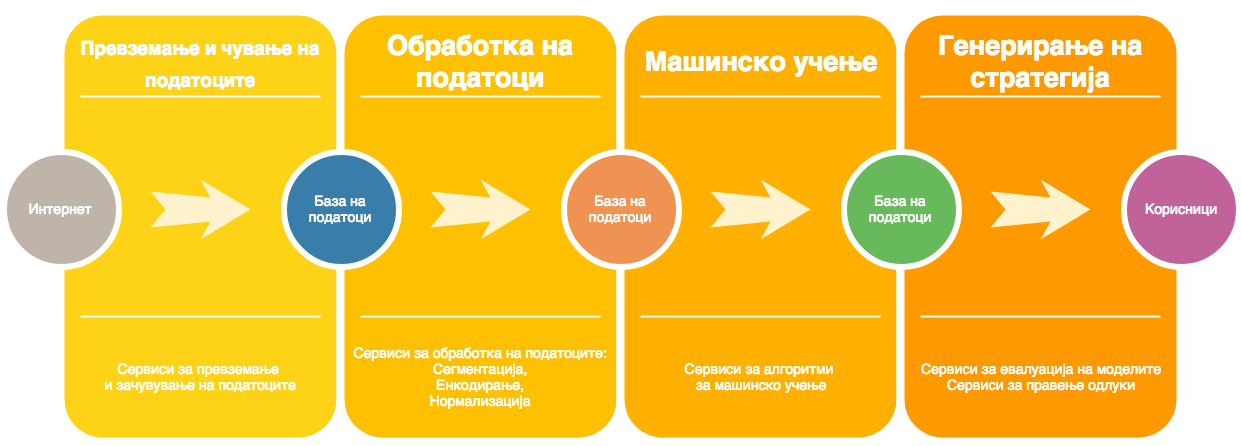
\includegraphics[scale=0.34]{images/Tek_na_podatocite.png}
\caption{Дефинирање на тек на податоци}
\label{fig:tek}
\centering
\end{figure}

\subsection{Справување со тесни грла}
За да можеме системот да го направиме скалабилен прво треба да разгледаме каде би имале тесни грла. Според ограничувањата кои ги разгледавме и апстрактниот дизајн можеме да заклучиме дека најочигледните тесни грла во системот се превземањето на податоците и тренирањето на моделите за машинско учење. За справување со овие проблеми предлагаме паралелизација на роботот за превземање на податоци и паралелизација на тренирањето на моделите. Со тоа системот би изгледал како на слика \ref{fig:system}. Ваквиот дизајн би ги елиминирал очигледните тесни грла кои би се јавиле во системот.

\begin{figure}[hbtp]
\centering
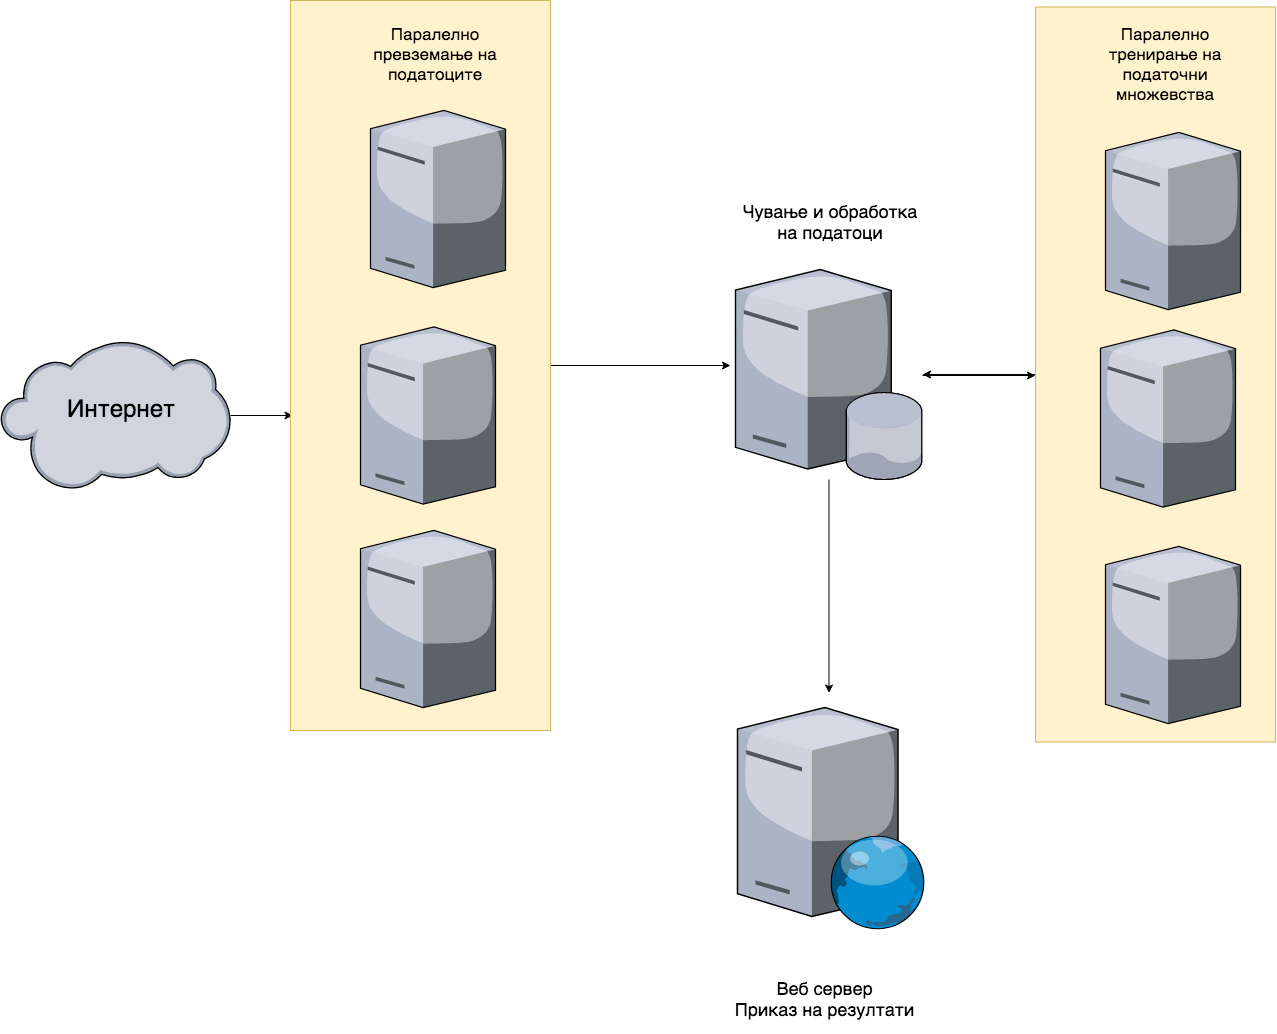
\includegraphics[scale=0.3]{images/system_design.png}
\caption{Дизајн на систем за препораки  за обложување на спортски натпревари}
\label{fig:system}
\end{figure}

\chapter{\mbox{Превземање и обработка на податоци}}
\label{sec:data}
\section{Превземање на податоците}
Алгоритмите за машинско учење учат од податоци. Затоа е важно пред било што во системот да имаме податоци за тренирање на алгоритмите. За нашиот систем одлучивме да користиме податоци од фудбалски натпревари и како едни од главните атрибути ќе ги земеме квотите за обложување доделни од обложувалниците. Постојат повеќе начини на внесување на овој тип на податоци во нашиот систем, но ние ќе се задржиме на три: консумирање на веб сервиси, запишување од датотеки и превземање од интернет страници. Во прилог ќе ги предностите и недостатоците на овие типови на внесувања и кои се нивните предности и недостатоци.  
\subsection{Консумирање на сервиси}
Како еден од најлесните методи на превземање на податоци е консумирањето на веб сервиси. Постојат повеќе платформи што ја нудат оваа опција како за историски податоци така и за податоци во реално време. Бизнис моделот на сите платформи им е продажбата на овие сервиси и бидејќи како што кажавме во првото поглавје обложувањето на спортски натпревари е бизнис од 452 милијарди долари ваквите сервиси се се скапи. Предноста на користење на овој метод за внесување на податоци e тоа што сервисите лесно се конзумираат и податоците се веродостојни. Иако оваа опција од технички аспект е најдобра, од финансиски причини одлучивме за изработката на магистерскиот труд да не ја користиме.  
\subsection{Запишување од датотеки}
Друг метод на внесување на податоци е сериско запишување. Со овој метод е добар за превземање на историските податоци, но не можеме да превземаме податоци во реално време и можно е ограничување на натпреварите на само одредени фудбалски лиги. За нашиот систем ние ги превземавме историските податоци од \cite{football-data} и предноста на овој метод е што податоците се структурирани и може лесно да се внесат во системот. Со овој метод внесовме само 5000 историски податоци за фудбалски натпревари. Останатите податоци го внесуваме преку превземање од интернет страници.
\subsection{Превземање од интернет страници}
Најголемиот дел од податоците што ги внесуваме ви системот е преку превземање од интернет страници. Креиравме робот во Python програмскиот јазик кој прво ги превзема историските податоци од претходните натпревари, а потоа секојдневно превзема податоци за нови натпревари. За развивање на ваквиот софтвер како основа го земавме роботот од \cite{mingov2016application} и го адаптиравме да превзема податоци од неколку веб страници кои прикажуваат податоци за натпревари во реално време. Недостатоците на овој метод на внесување на податоци се дека превземањето и слекцијата на податоците е доста тешка и треба проучување на структурата на веб страната за да можеме да ги одбереме соодветните податоци. Содржината на веб страниците може да биде доста динамична и мала промена на кодот од нивна страна може да влијае на перформансите на роботот. Некои страни ги прикажуваат податоците динамички преку конзумирање на веб сервиси и со тоа се воведува задоцнување. За да се справиме со ваквите проблеми користевме библиотека за автоматизација на веб-прелистувачи \cite{wang2012test} што ги "мами" серверите дека кон нив пристапуваат реални корисници. Со ваквиот начин превземањето на податоците за еден натпревар може да биде во опсег од 3 до 6 секунди. Во претходното поглавје зборувавме за ограничувањата на системот и напоменавме дека постои тесно грло пре превземањето на податоците. Со пресметката од ограничувањата, за превземање на историските податоци потребни се 55 часа, но со паралелизација на повеќе нитки успеавме да превземеме 49000 историски податоци за натпревари за помалку од 10 часа.
\subsection{Чување на податоците}
За да ги зачуваме податоците користиме PostgreSQL \cite{momjian2001postgresql} база на податоци. Податоците од секој натпревар ги внесуваме во табела Натпревар и за секој натпревар чуваме кои тимови играат, во кое време и во која лига, квотите од обложувалниците и резултатите од натпреварот. На слика \ref{fig:eadiagram} е прикажан ЕА дијаграм од базата на податоци, освен Натпревар во системот имаме уште шест табели: Регион, Земја, Лига, Тим, Асоцијација и Спорт. 

\begin{figure}[hbtp]
\centering
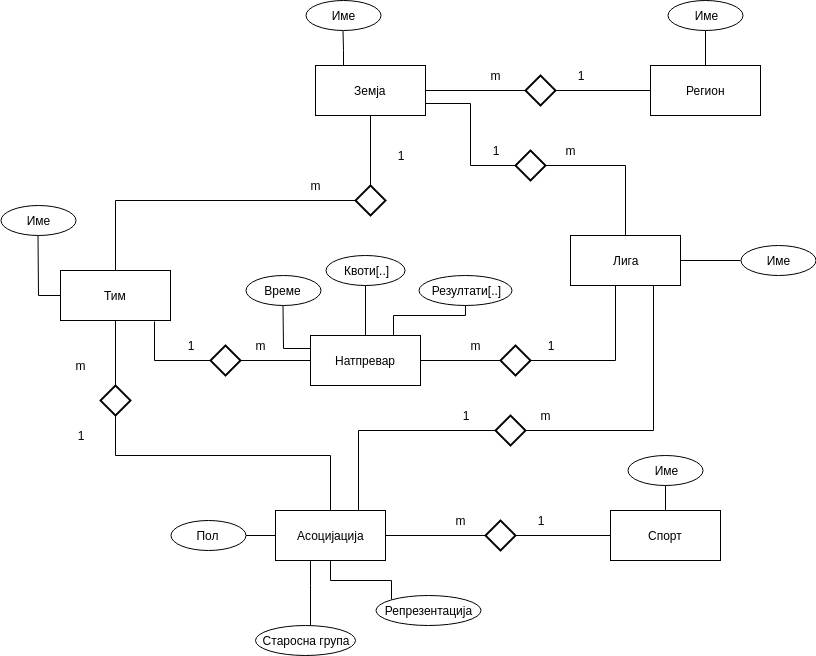
\includegraphics[scale=0.4]{images/EA-diagram.png}
\caption{ЕА дијаграм од базата на податоци}
\label{fig:eadiagram}
\end{figure}

Во табелите Регион и Земја чуваме локациски информации Регион ги соджи континентите во светот, додека Земја ги содржи сите земји. Тим ги содржи сите информации за еден тим, а Лига информациите за лигите во кои се одигруваат натпреварите. Во табелата Асоцијација чуваме податоци за полот и старосната група на еден тим и тоа дали е репрезентација или не. Тимовите може да играат натпревари само во асоцијацијата на која праипаѓаат и во Спорт чуваме податоци на кој спорт припаѓа асоцијацијата.

\section{Обработка и филтрирање}
Многу е важно да ги имаме вистинските податоци за проблемот што сакаме да го решиме. Дури и ако имаме добри податоци, треба да бидеме сигурни дека тие се во корисен формат, скалирани, па дури и дека значајните атрибути се вклучени.
\subsection{Селекција на атрибути}
Целта на овој чекор е да селектираме подмножество од сите достапни податоци со кои ќе работиме. Притоа треба да внимаваме дали некој атрибут има премногу податоци што недостасуваат што би го направиле лош претставник за понатамошната обработка.

Во нашето податочно множество поголемиот дел од атрибутите се обложувачките квоти, освен нив како атрибути ги земаме времето на одигрувањето на натпреварот, тимовите кои се натпреваруваат и лигата во која се натпреваруваат. Со ова податочното множество има 52 атрибути.
\subsection{Изведени атрибути}
Изведени атрибути се атрибути изведени од други податоци користејќи математичка, логичка или некаков друг вид на трансформација.

Во нашиот случај со помош на пребарување врз базата на податоци изведуваме атрибути од резултатите од претходните одиграни натпревари за секој тим како на пример број на дадени голови, број на примени голови. број на победи и порази итн. Освен тоа за секој натпревар вадиме статистика за сите претходни одиграни натпревари меѓу двата тима. Со овие изведени податоци нашето множество вкупно брои 91 атрибут. 
\subsection{Сегментација на множеството}
Сегментацијата на податоците е трансформација која се применува врз дадено множество со цел да добиеме податоци со слични карактеристики. Во нашето множество имаме 54387 натпревари, но ако ја погледнеме нивната распределба на слика \ref{fig:raspredelba} заклучуваме дека повеќето одиграни натпревари се од последните неколку месеци што значи дека имаме мал број на историски податоци што може да ги користиме во тренинг множеството и голем број на нови натпревари што ќе бидат во тест множеството. 
\begin{figure}[hbtp]
\centering
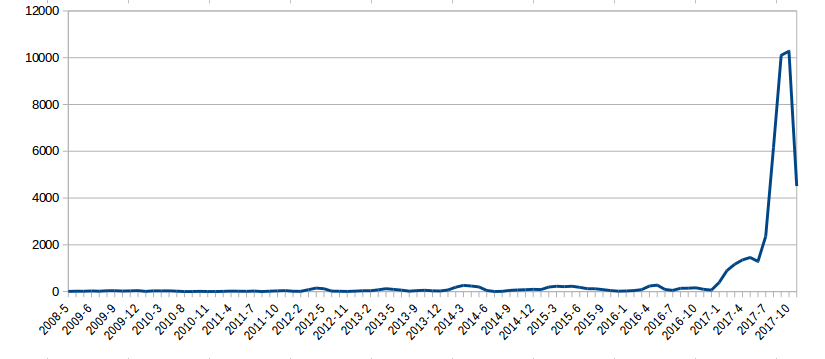
\includegraphics[scale=0.4]{images/raspredelba.png}
\caption{Распределба на одиграни натпревари}
\label{fig:raspredelba}
\end{figure}

Првата сегментација на множеството што ќе ја направиме е сегментација по асоцијација, во предвид ќе ги земеме само натпреварите што имаат асоцијација: мажи, сениори, клупски тимови. Со ваквата трансформација бројот на натпревари се намали на 45743. Поради ваквата распределба на натпреварите и заради тоа што сакаме да ја запазиме хронологијата на податоците, треба да го поделиме множеството на 4 дела: историски податоци, тренинг множество, валидациско множество и тест множество. Историските податоци нема да бидат вклучени во множеството, нив ги занемаруваме со цел да добиеме тренинг множество со добри изведени атрибути. Со тренинг множеството ги тренираме нашите модели, а валидациското множество ќе го користиме при селекција на параметри за моделите. На крај нашите модели ќе ги евалуираме на тест множеството. За нашето истражување направивме 3 групи опсези на поделба на множеството по датуми соодветно. Дополнително вклучивме и уште 4 начини на поделба: сите натпревари, натпревари од тимови кои ги има само во историските и тренинг множества, само тимови кои имаат повеќе од 25 натпревари и тимови кои имаат повеќе од 25 натпревари и ги има само во историските и тренинг множества. Кога ќе ги примениме и трите групи на опсези на овие начини на поделба добиваме 12 множества. За експериментирање одредивме по 4 типа на класификации за секое множество: некој тим ќе победи или е нерешено, домашниот тим победува или не, двата тима ќе поентираат и бројот на голови е парен или непарен.  Со што бројот на множества за тренирање ни се искачи на 48. И последната сегментација што ја применивме е сегментација на натпреварите од само една лига - Англиската премиер лига. Овде не ги применивме опсезите и начините на поделба, во овој случај ја земавме последната сезона да биде тест множество, претпоследната валидациско и останатите 12 сезони како тренинг множество. За оваа сегментација користевме само 2 типа на класификација: некој тим ќе победи или е нерешено, домашниот тим победува или не. Со тоа конечниот број на податочни множества ни достигна до 50. На табела \ref{table:datasets} се прикажани сите изведени множества.

\begin{table}[hbtp]
 \centering
 \scalebox{0.5}{%
 \begin{tabular}{| c | c | c |}
 \hline
 колонa & вредност & опис \\ 
 \hline
 начин & начин 1 & сите натпревари \\
 начин & начин 2 & натпревари од тимови кои ги има само во историските и тренинг множества \\
 начин & начин 3 & само тимови кои имаат повеќе од 25 натпревари \\
 начин & начин 4 & тимови кои имаат повеќе од 25 натпревари и ги има само во историските и тренинг множества \\
 начин & начин 5 & Англиската премиер лига \\
 опсег & опсег 1 & [2014-07-01, 2015-06-30] [2015-07-01, 2016-06-30] [2016-07-01, 2017-11-22] \\
 опсег & опсег 2 & [2015-07-01, 2016-06-30] [2016-07-01, 2017-06-30] [2017-07-01, 2017-11-22] \\
 опсег & опсег 3 & [2016-07-01, 2017-06-30] [2017-07-01, 2017-09-30] [2017-10-01, 2017-11-22] \\
 опсег & опсег 4 & [2004-08-13, 2016-05-16] [2016-08-12, 2017-05-21] [2017-08-10, 2018-02-24]\\
 класа & 1x2 & некој тим ќе победи или е нерешено \\
 класа & 1 or x2 & домашниот тим победува или не \\
 класа & bts &  двата тима ќе поентираат \\
 класа & odd even & бројот на голови е парен или непарен \\
 \hline
\end{tabular}}


\scalebox{0.7}{%
\begin{tabular}{| c | c | c | c | c | c | c | c | }
\hline
број &начин & опсег & класа & тренинг мн. & валидациско мн. & тест мн. & вкупно \\
\hline
 1 & начин 1 & опсег 1 & 1x2 & 891 & 616 & 27052 & 28559\\
 2 & начин 1 & опсег 1 & 1 or x2 & 891 & 616 & 27052 & 28559\\
 3 & начин 1 & опсег 1 & bts & 891 & 616 & 27052 & 28559\\
 4 & начин 1 & опсег 1 & odd even & 891 & 616 & 27052 & 28559\\
 5 & начин 1 & опсег 2 & 1x2 & 616 & 4732 & 22320 & 27668\\
 6 & начин 1 & опсег 2 & 1 or x2 & 616 & 4732 & 22320 & 27668\\
 7 & начин 1 & опсег 2 & bts & 616 & 4732 & 22320 & 27668\\
 8 & начин 1 & опсег 2 & odd even & 616 & 4732 & 22320 & 27668\\
 9 & начин 1 & опсег 3 & 1x2 & 4732 & 12969 & 9351 & 27052\\
 10 & начин 1 & опсег 3 & 1 or x2 & 4732 & 12969 & 9351 & 27052\\
 11 & начин 1 & опсег 3 & bts & 4732 & 12969 & 9351 & 27052\\
 12 & начин 1 & опсег 3 & odd even & 4732 & 12969 & 9351 & 27052\\
 13 & начин 2 & опсег 1 & 1x2 & 891 & 298 & 1146 & 2335\\
 14 & начин 2 & опсег 1 & 1 or x2 & 891 & 298 & 1146 & 2335\\
 15 & начин 2 & опсег 1 & bts & 891 & 298 & 1146 & 2335\\
 16 & начин 2 & опсег 1 & odd even & 891 & 298 & 1146 & 2335\\
 17 & начин 2 & опсег 2 & 1x2 & 616 & 444 & 1347 & 2407\\
 18 & начин 2 & опсег 2 & 1 or x2 & 616 & 444 & 1347 & 2407\\
 19 & начин 2 & опсег 2 & bts & 616 & 444 & 1347 & 2407\\
 20 & начин 2 & опсег 2 & odd even & 616 & 444 & 1347 & 2407\\
 21 & начин 2 & опсег 3 & 1x2 & 4732 & 4878 & 2309 & 11919\\
 22 & начин 2 & опсег 3 & 1 or x2 & 4732 & 4878 & 2309 & 11919\\
 23 & начин 2 & опсег 3 & bts & 4732 & 4878 & 2309 & 11919\\
 24 & начин 2 & опсег 3 & odd even & 4732 & 4878 & 2309 & 11919\\
 25 & начин 3 & опсег 1 & 1x2 & 338 & 155 & 2828 & 3321\\
 26 & начин 3 & опсег 1 & 1 or x2 & 338 & 155 & 2828 & 3321\\
 27 & начин 3 & опсег 1 & bts & 338 & 155 & 2828 & 3321\\
 28 & начин 3 & опсег 1 & odd even & 338 & 155 & 2828 & 3321\\
 29 & начин 3 & опсег 2 & 1x2 & 155 & 1195 & 1633 & 2983\\
 30 & начин 3 & опсег 2 & 1 or x2 & 155 & 1195 & 1633 & 2983\\
 31 & начин 3 & опсег 2 & bts & 155 & 1195 & 1633 & 2983\\
 32 & начин 3 & опсег 2 & odd even & 155 & 1195 & 1633 & 2983\\
 33 & начин 3 & опсег 3 & 1x2 & 1195 & 1100 & 533 & 2828\\
 34 & начин 3 & опсег 3 & 1 or x2 & 1195 & 1100 & 533 & 2828\\
 35 & начин 3 & опсег 3 & bts & 1195 & 1100 & 533 & 2828\\
 36 & начин 3 & опсег 3 & odd even & 1195 & 1100 & 533 & 2828\\
 37 & начин 4 & опсег 1 & 1x2 & 338 & 101 & 618 & 1057\\
 38 & начин 4 & опсег 1 & 1 or x2  & 338 & 101 & 618 & 1057\\
 39 & начин 4 & опсег 1 & bts  & 338 & 101 & 618 & 1057\\
 40 & начин 4 & опсег 1 & odd even  & 338 & 101 & 618 & 1057\\
 41 & начин 4 & опсег 2 & 1x2 & 155 & 225 & 576 & 956\\
 42 & начин 4 & опсег 2 & 1 or x2 & 155 & 225 & 576 & 956\\
 43 & начин 4 & опсег 2 & bts & 155 & 225 & 576 & 956\\
 44 & начин 4 & опсег 2 & odd even & 155 & 225 & 576 & 956\\
 45 & начин 4 & опсег 3 & 1x2 & 1195 & 1058 & 512 & 2765\\
 46 & начин 4 & опсег 3 & 1 or x2 & 1195 & 1058 & 512 & 2765\\
 47 & начин 4 & опсег 3 & bts & 1195 & 1058 & 512 & 2765\\
 48 & начин 4 & опсег 3 & odd even & 1195 & 1058 & 512 & 2765\\
 49 & начин 5 & опсег 4 & 1x2 & 4560 & 380 & 279 & 5219 \\
 50 & начин 5 & опсег 4 & 1 or x2 & 4560 & 380 & 279 & 5219 \\
\hline
\end{tabular}}
\caption{Изведени множества за тренирање}
\label{table:datasets}
\end{table}

\section{Трансформација на податоците}
Последниот чекор што ќе го превземеме при обработката на податоците е трансформацијата. Алгоритмите со којшто ќе работиме и доменот на проблемот ќе влијаат на овој чекор и многу веројатно ќе треба да ги ревидираме различните трансформации на нашите препроцесирани податоци додека работиме на нашиот проблем.
\subsection{Кодирање}
Кодирање или продолжување е трансформација на категорични променливи на бинарни или нумерички. Категориските променливи мора да бидат кодирани во многу методи за моделирање. Два главни типа на кодирање се бинарно и класно.

\subsubsection{Бинарно кодирање}
Нумерирање на категориски променливи со земање на вредности 0 или 1 за да укаже на отсуство или присуство на секоја категорија. Ако категориската променлива има k категории, ќе треба да создадеме k бинарни променливи. Главниот недостаток со овој метод е кога категориска променлива со многу вредности (на пример, тимови), која може значително да ја зголеми димензијата на податоците. Во нашиот случај овој тип на кодирање можеме да го примениме само во множествата под број 49 и 50 од табела \ref{table:datasets}. Во другите множества бројот на тимови е поголем и со тоа може значитено да се зголеми бројот на атрибути.
\subsubsection{Класно кодирање}
Класното кодирање е нумерирање на категорични променливи преку класата. Во овој метод, ние ја заменуваме категориската променлива со само една нова нумеричка променлива и ја заменуваме секоја категорија на категориска променлива со соодветната веројатност на класата. Главните недостатоци на овој метод се нејзината зависност од дистрибуцијата на класата и нејзината пониска моќ на предвидување во споредба со бинарниот метод на кодирање.
\subsection{Нормализација}
Откако ќе ги трансформираме сите податоци на множеството во нумерички потребно е да направиме скалирање на податоците во даден опсег овој процес се вика нормализација. За нашиот проблем ние ќе примениме две различни нормализации: нормализација по стандардна девијација и min-max нормализација во опсег од 0 до 1. 
\section{Обработени податоци и следни чекори}
Во ова поглавје ги разгледавме чекорите за превземање и обработка на податоците, увидовме на потребните чекори потребни за да направиме добри множества и како да ги трансформираме податоците за да можеме да добиваме подобри резултати со алгоритмите за машинско учење. Во следното поглавје ќе рагледаме дел од нив.    
\chapter{Алгоритми за машинско учење}
\label{sec:machine_learning}
Постојат многу алгоритми за машинско учење и ако би ги именувале сите би изгледале премногу и не би знаеле да одбереме соодветен доколку не би направеле некакво групирање. Најчести групирања со кои можеме да се сретнеме се групирање по сличност по форма и функција и групирање по начин на учење. И двата пристапи се корисни, но ќе се фокусираме групирањето по начин на учење со цел да најдеме соодветни алгоритми за решавање на начиот проблем. 
Постојат различни начини на кои алгоритам може да се моделира проблем врз основа на неговата интеракција со искуството или околината или она што сакаме да го наречеме влезни податоци.
Популарно е во машинското учење да се разгледаат начините за учење кои еден алгоритам може да го усвои.
Постојат само неколку главни начини на учење или модели за учење кои еден алгоритам може да ги има: надгледувано учење, ненадгледувано учење и полу-надгледувано учење.
Оваа таксономија или начинот на организирање алгоритми за машинско учење е корисна затоа што не да размислуваме за улогите на влезните податоци и за процесот на подготовка на модел и одбереме оној кој е најсоодветен за нашиот проблем за да го добиете најдобриот резултат.

Кај надгледуваното учење влезните податоци се нарекуваат тренинг податоци и имаат позната класа или резултат како што се спам / не-спам или цената на акциите во одредено време.
Моделот се подготвува преку процес на обука во кој е потребно да се направат предвидувања и се корегира кога тие предвидувања се погрешни. Процесот на обука продолжува додека моделот не постигне посакувано ниво на точност на податоците за обуката.
Проблеми кои се решаваат со надгледуваното учење се класификација и регресија.

Кај ненадгледуваното учење влезните податоци не се етикетирани и немаат познат резултат.
Моделот се подготвува со издвојување на структури присутни во влезните податоци. На овој начин може да се извлечат општи правила за податоците. Тоа може да биде преку математички процес, или може да биде да се организираат податоци по сличност.
Проблеми кои се решаваат со ненадгледуваното учење се кластерирање, намалување на димензионалноста и учење на правила за здружување.

Кај полу-надгледуваното учење влезните податоци се мешавина од етикетирани и неетикетирани примери.
Овде моделот мора да ги научи структурите за организирање на податоците, како и да направи предвидувања.
Проблеми кои се решаваат со надгледуваното учење се исто така класификација и регресија.

Во нашиот случај треба да решиме проблем на класифицирање и имаме познати класи за сите влезни податоци, затоа проблемот ќе го дефинираме како надгледувано учење. Пред да се врутниме кон решавање на проблемот со помош на вештачки невронски мрежи, ќе разгледаме неколу алгоритми за надгледувано учење и како тие го решаваат нашиот проблем.  
\section{Алгоритми за надгледувано учење}
\subsection{Наивен баесов класификатор}
Наивниот баесов класификатор \cite{rish2001empirical} е класификациски алгоритам за бинарни и повеќе-класни класификациски проблеми.
Се нарекува наивен баесов класификатор, бидејќи пресметката на веројатностите за секоја хипотеза се поедноставени за да се направи нивната пресметка попрактична. Наместо да се обидуваат да ги пресметаат вредностите на секоја вредност на атрибутот P (d1, d2, d3 | h), се претпоставува дека се условно независни со оглед на целните вредности и се пресметуваат како P (d1 | h) * P (d2 | H) и и така натаму.
Ова е многу силна претпоставка која е малку веројатна кај реалните проблеми, односно дека атрибутите не си влијаат еден на друг.

На сликa \ref{fig:naive_bayes} се прикажани резултатите од тестирањето на сите податочни множества со наивен баесов класификатор поделени по класа. Најдобри резултати овој алгоритам постигнува кај множествата 49 и 50 дефинирани во табела \ref{table:datasets}, со 54.83\% за класифицирање на 1 Х 2 игра, односно 67.38\% за класифицирање на 1 или Х2 игра. 

\begin{figure}[H]
\centering
\begin{tabular}{cc}
  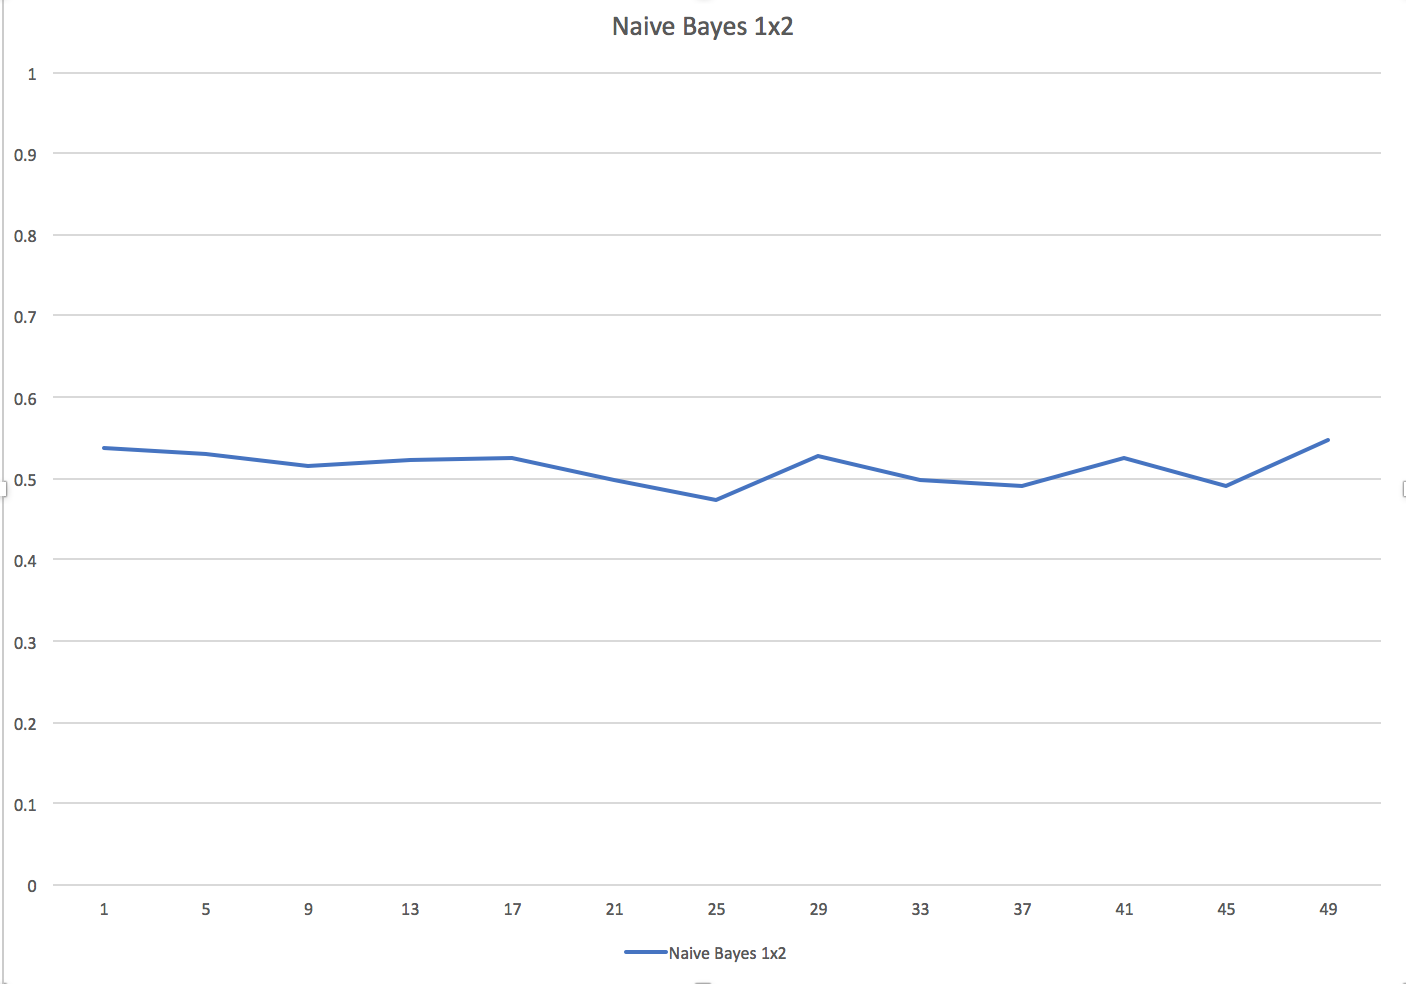
\includegraphics[width=8cm,height=5cm]{images/naive_bayes_1x2.png} &   
  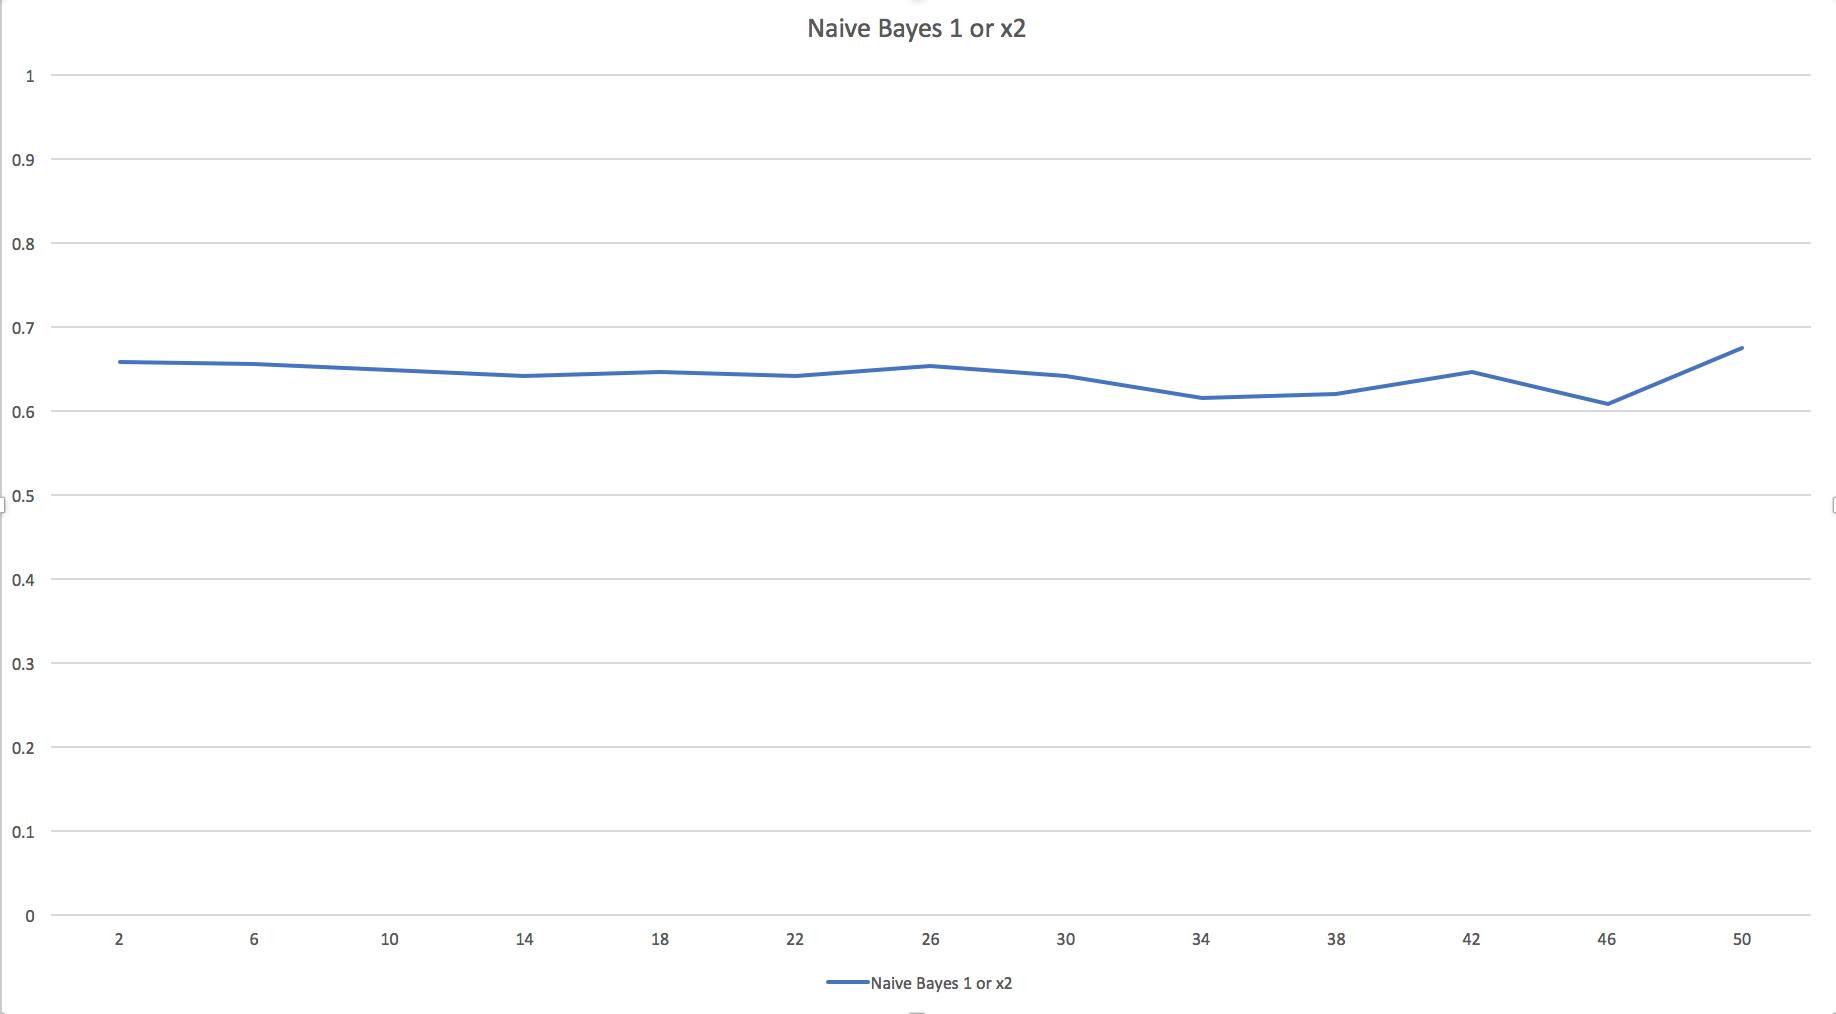
\includegraphics[width=8cm,height=5cm]{images/naive_bayes_1_or_x2.png} \\
(а) 1 Х 2 & (б) 1 или Х2 \\
 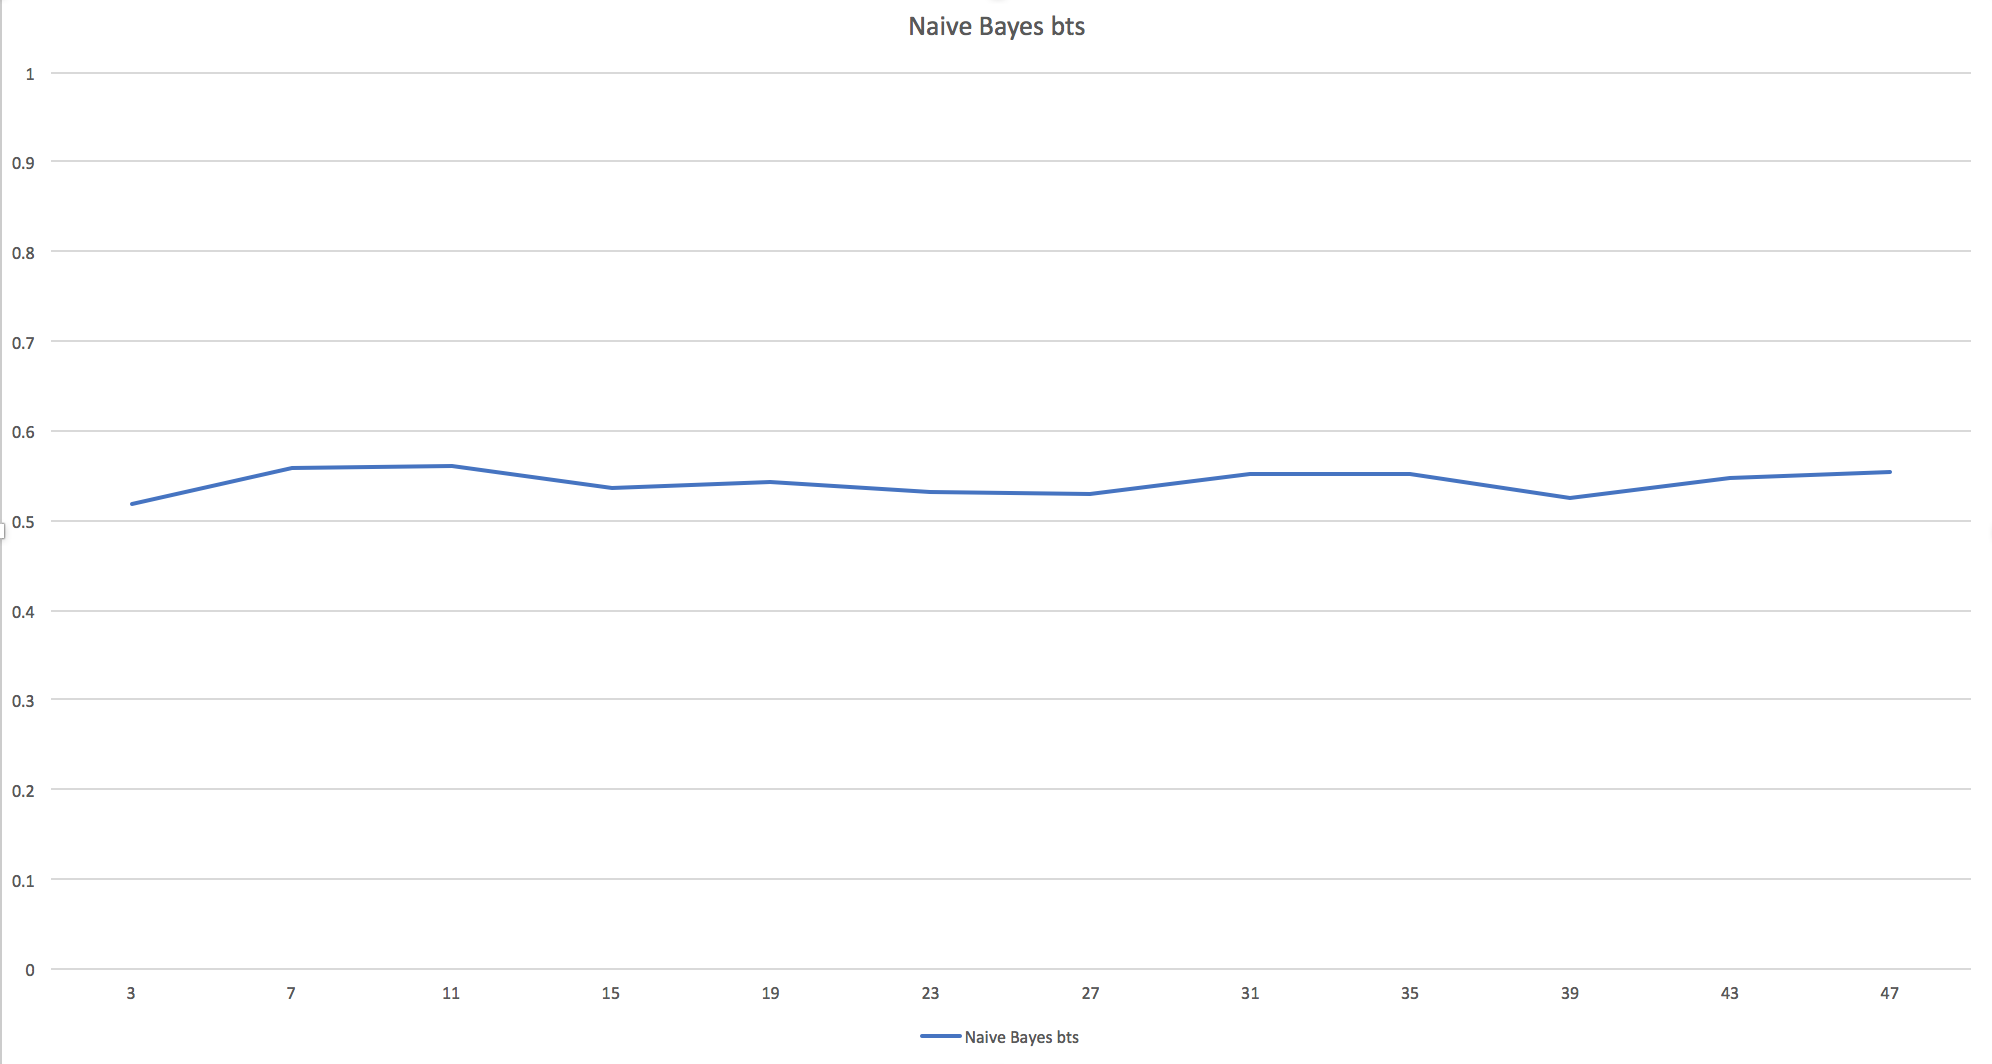
\includegraphics[width=8cm,height=5cm]{images/naive_bayes_bts.png}
 &   
 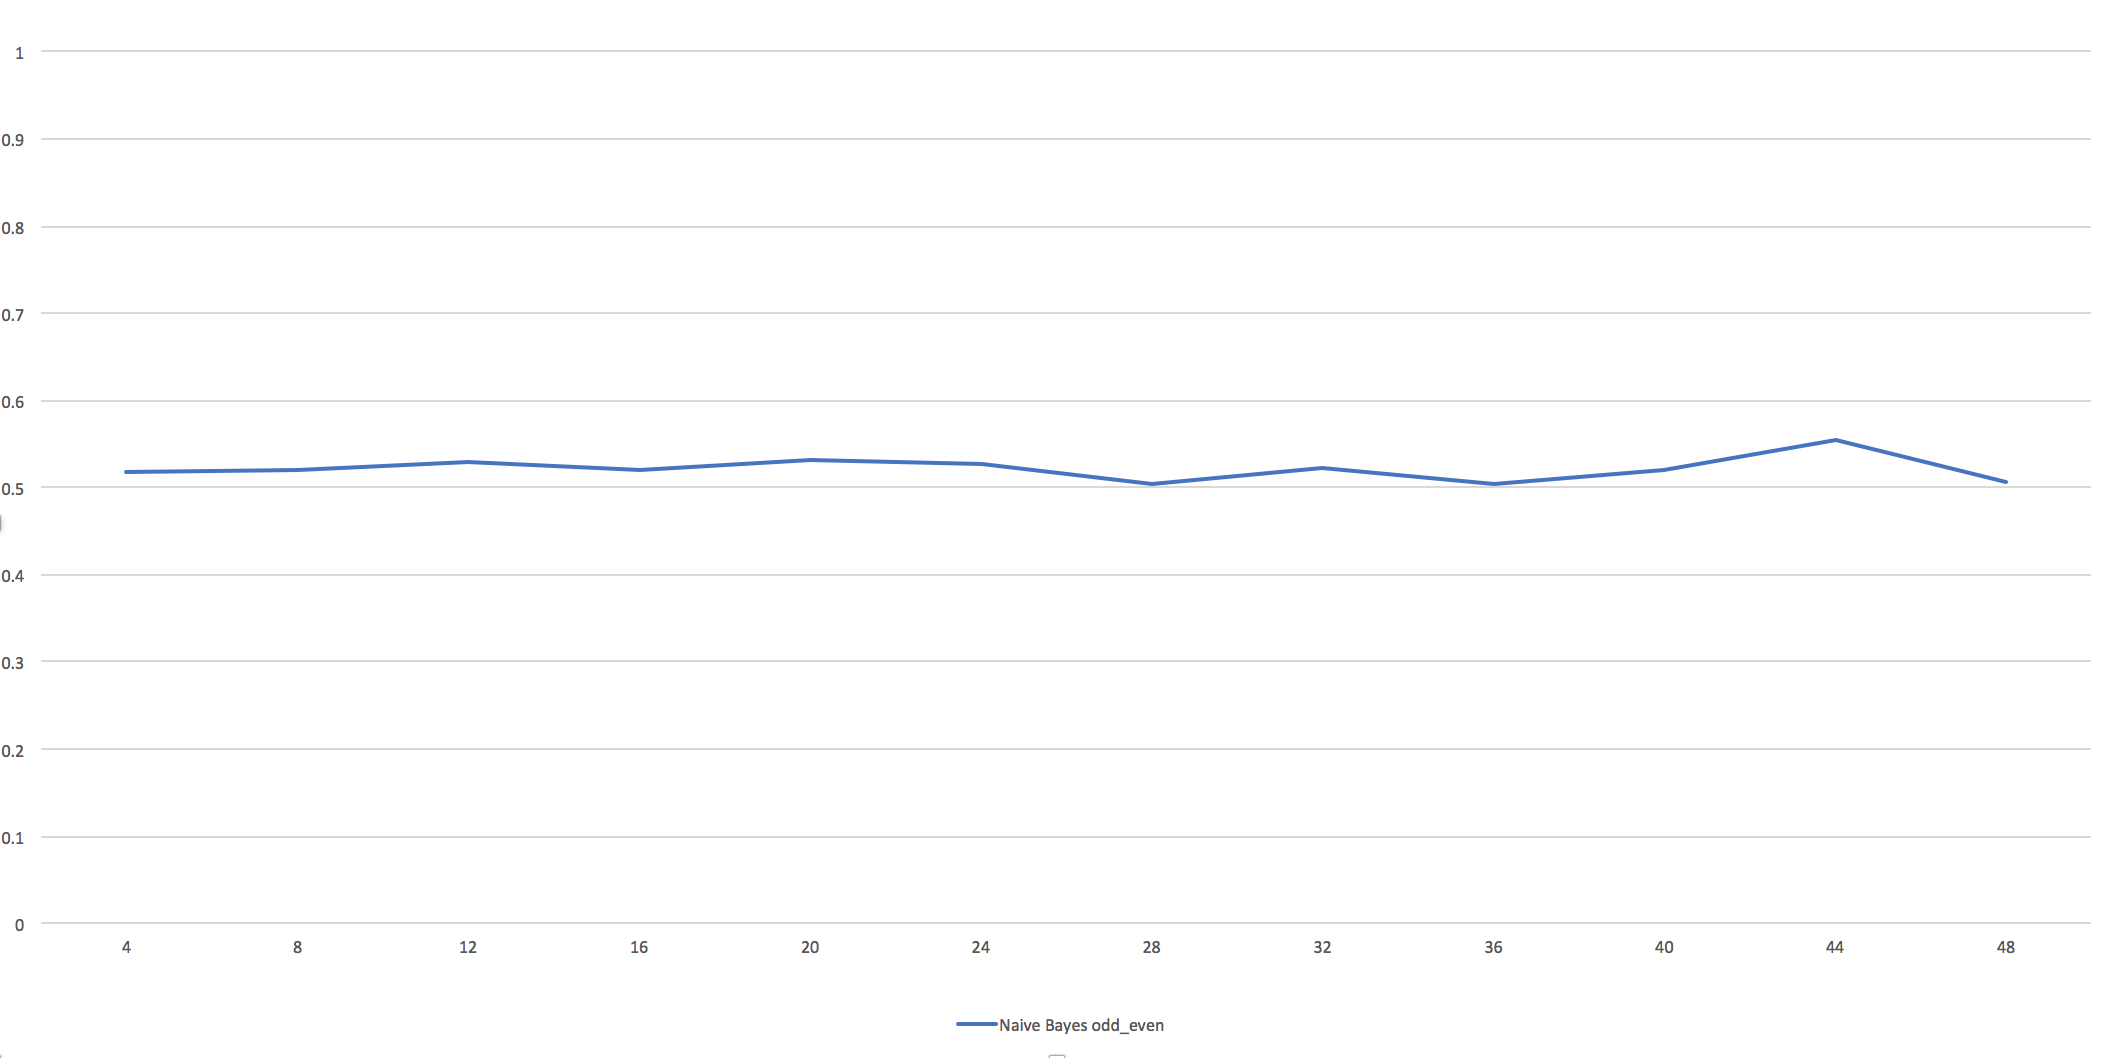
\includegraphics[width=8cm,height=5cm]{images/naive_bayes_odd_even.png} \\
(в) дали двата тима ќе поентираат & (г) парен/непарен број на голови \\
\end{tabular}
\caption{Резултати од тестирање со наивен баесов класификатор}
\label{fig:naive_bayes}
\end{figure}

\subsection{Логистичка регресија}
Логистичката регресија \cite{hosmer2013applied}, и покрај неговото име, е линеарен модел за класификација наместо регресија. Логистичката регресија е позната во литературата и како класификација на максимална ентропија или лог-линеарен класификатор. Во овој модел, веројатностите што ги опишуваат можните исходи на едно испитување се моделираат со помош на логистичка функција.
Логистичката функција, исто така наречена сигмоидна функција, била развиена од страна на статистичарите за да ги опише својствата на растот на популацијата во екологијата. Тоа е крива во форма на Ѕ (лат.), која може да земе реален број и да ја прикаже неговата вредност помеѓу 0 и 1.

На сликa \ref{fig:log_reg} се прикажани резултатите од тестирањето на сите податочни множества со логистичка регресија поделени по класа. Најдобри резултати овој алгоритам постигнува кај множествата 49 и 50 дефинирани во табела \ref{table:datasets}, со 54.83\% за класифицирање на 1 Х 2 игра, односно 67.74\% за класифицирање на 1 или Х2 игра.

\begin{figure}[H]
\centering
\begin{tabular}{cc}
  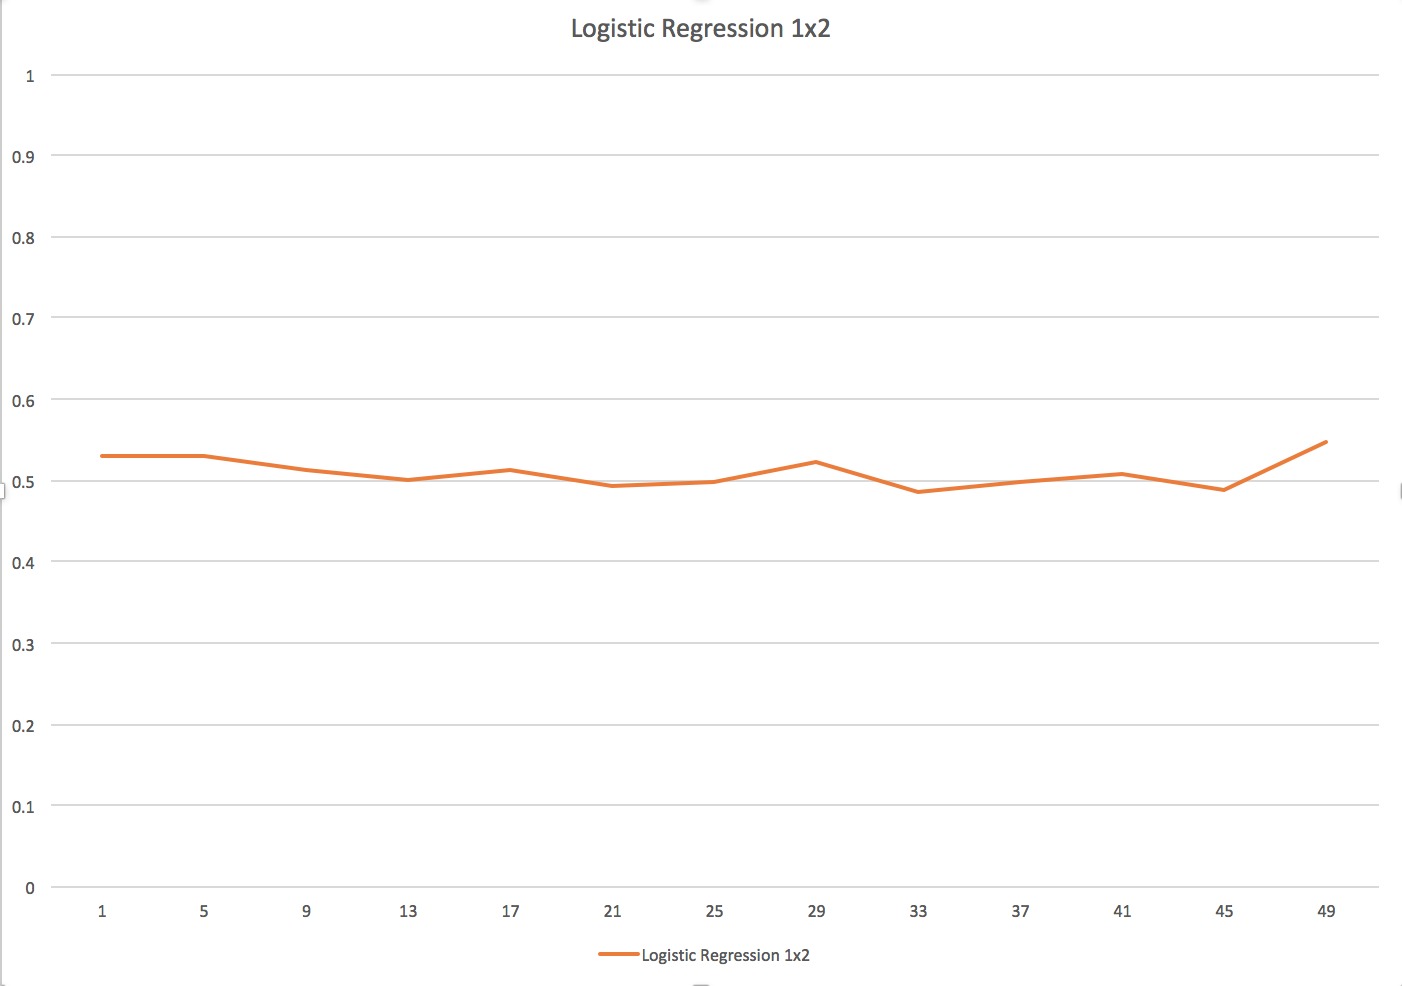
\includegraphics[width=8cm,height=5cm]{images/log_reg_1x2.png} &   
  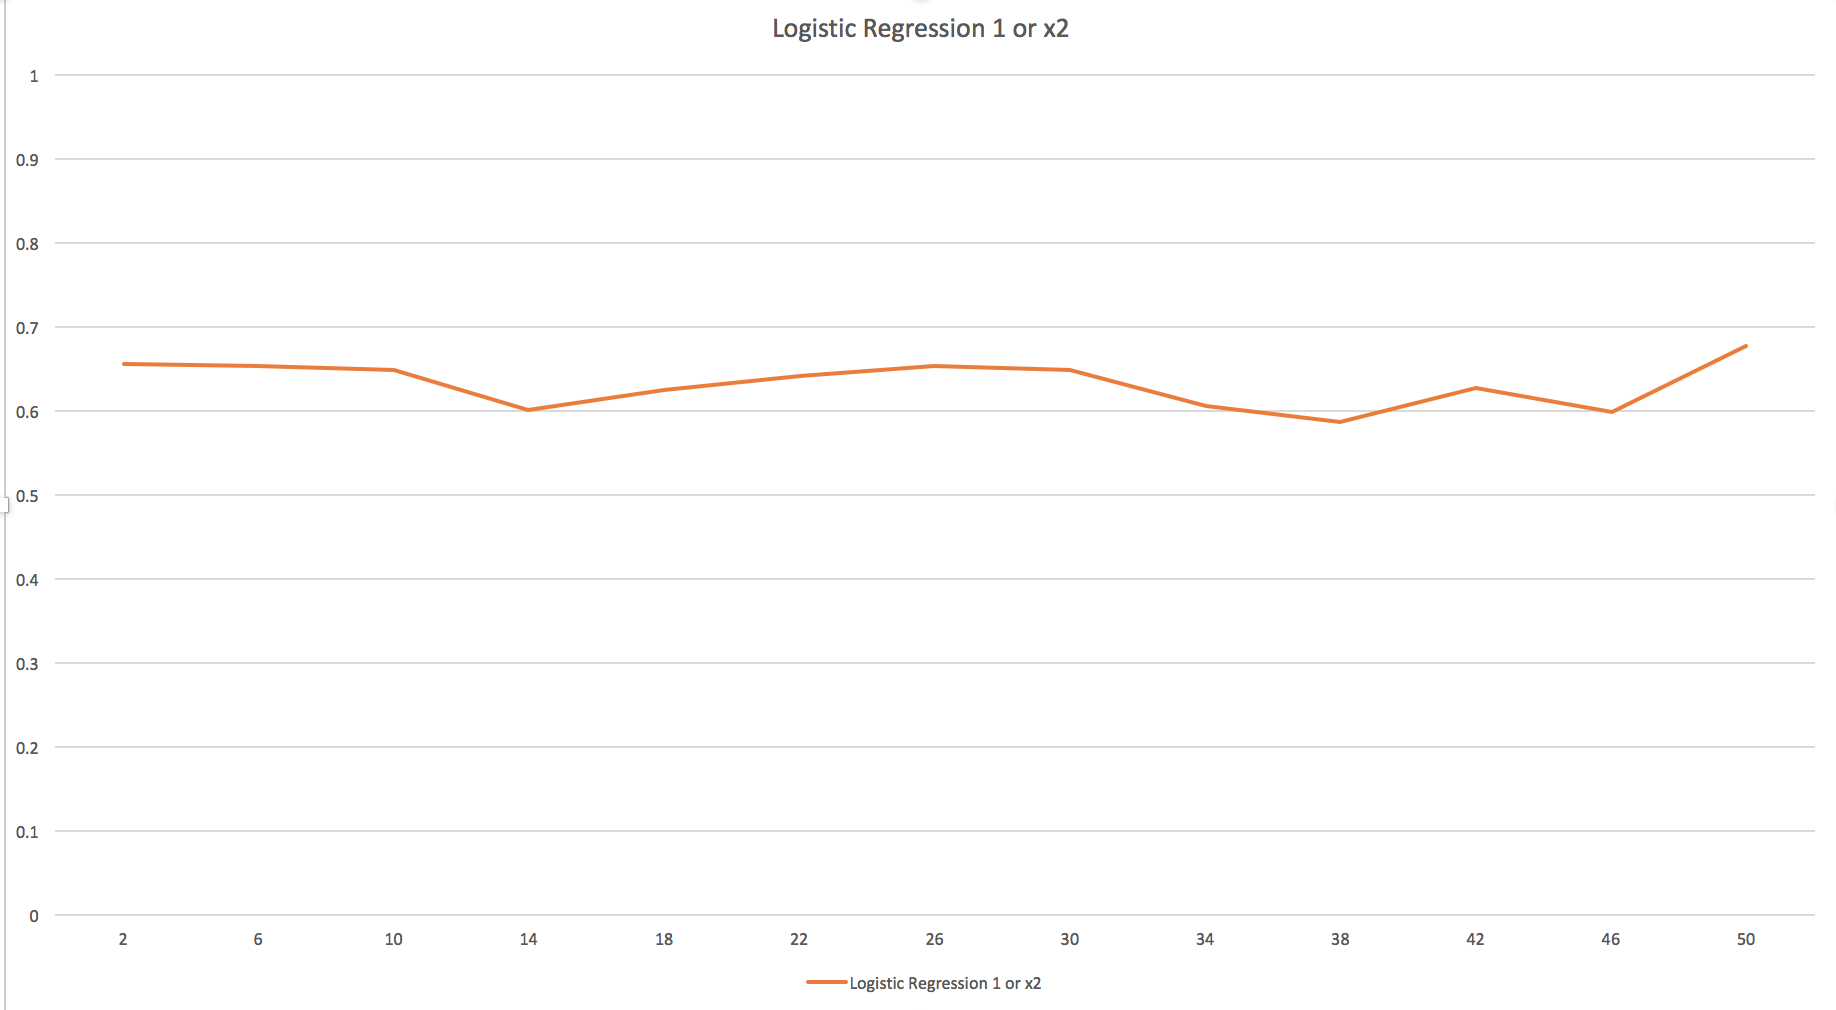
\includegraphics[width=8cm,height=5cm]{images/log_reg_1_or_x2.png} \\
(а) 1 Х 2 & (б) 1 или Х2 \\
 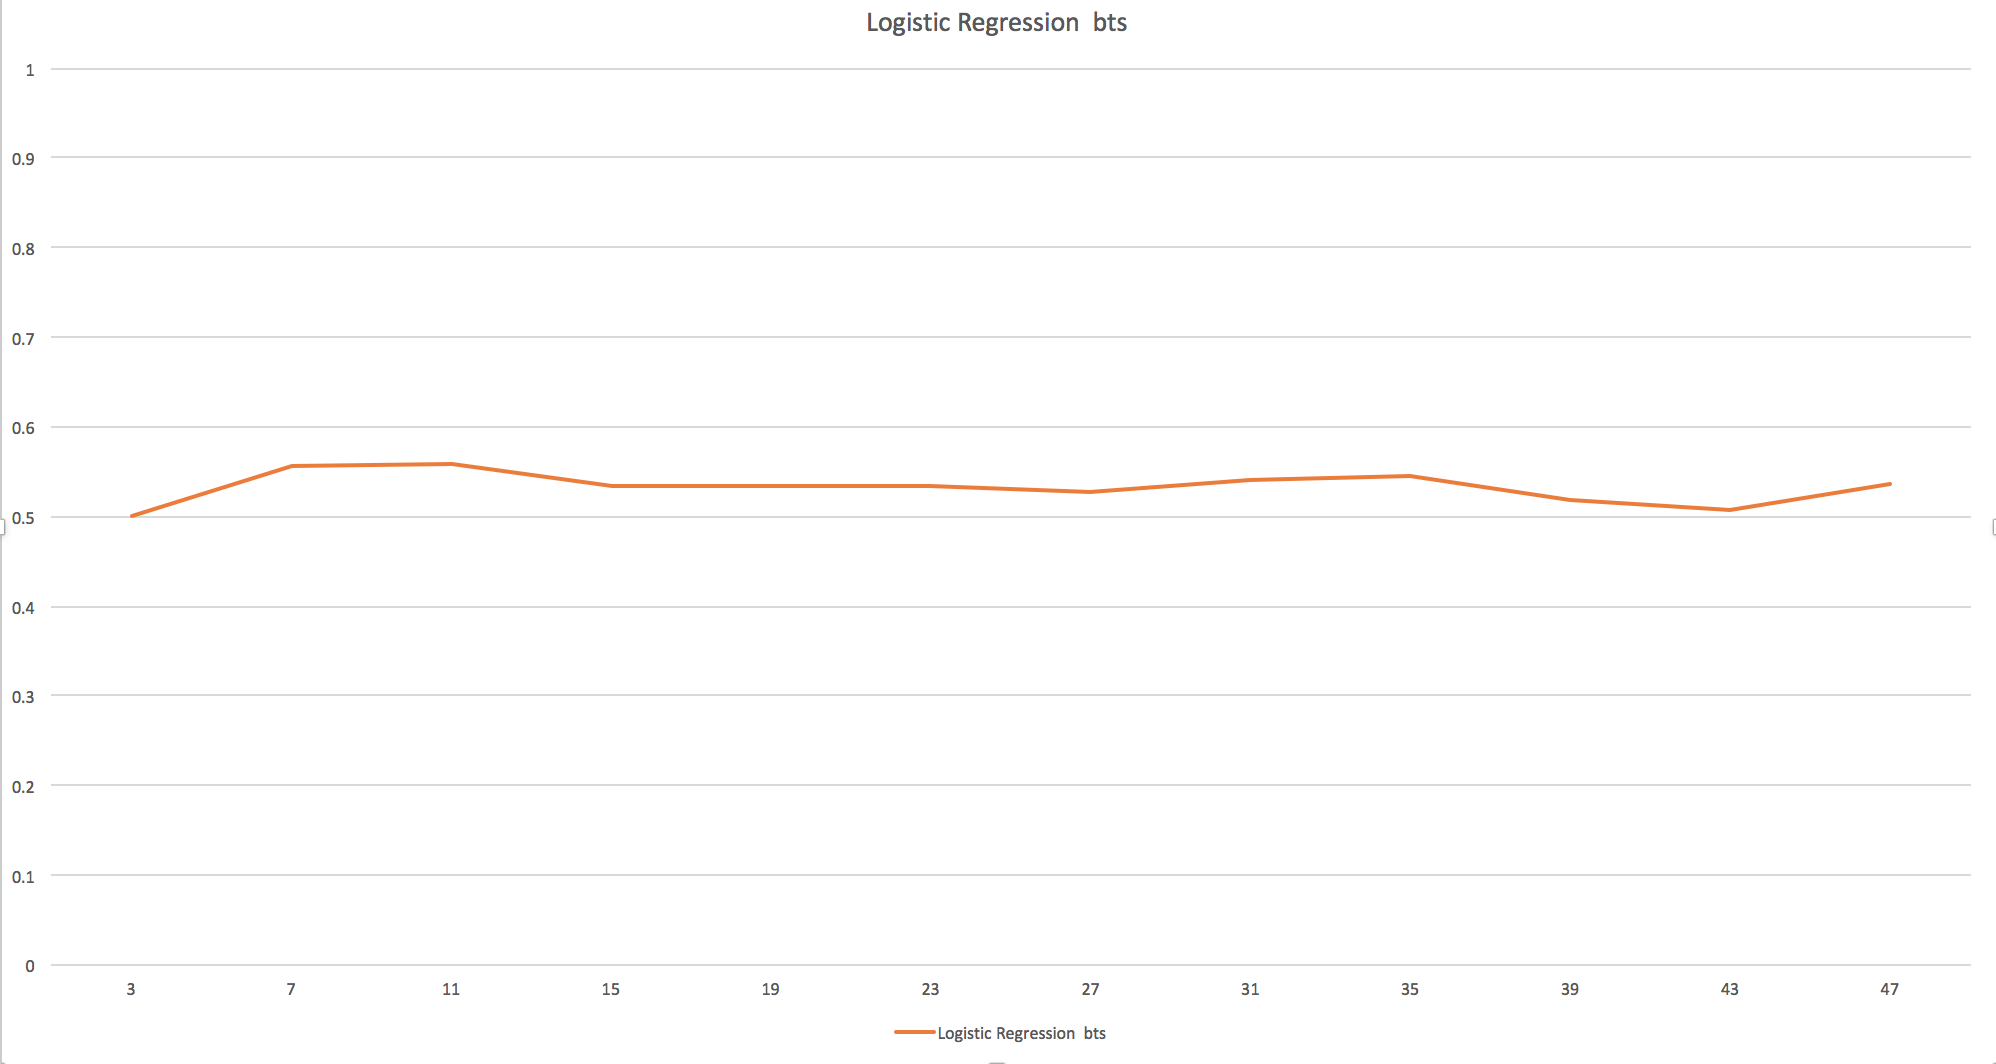
\includegraphics[width=8cm,height=5cm]{images/log_reg_bts.png}
 &   
 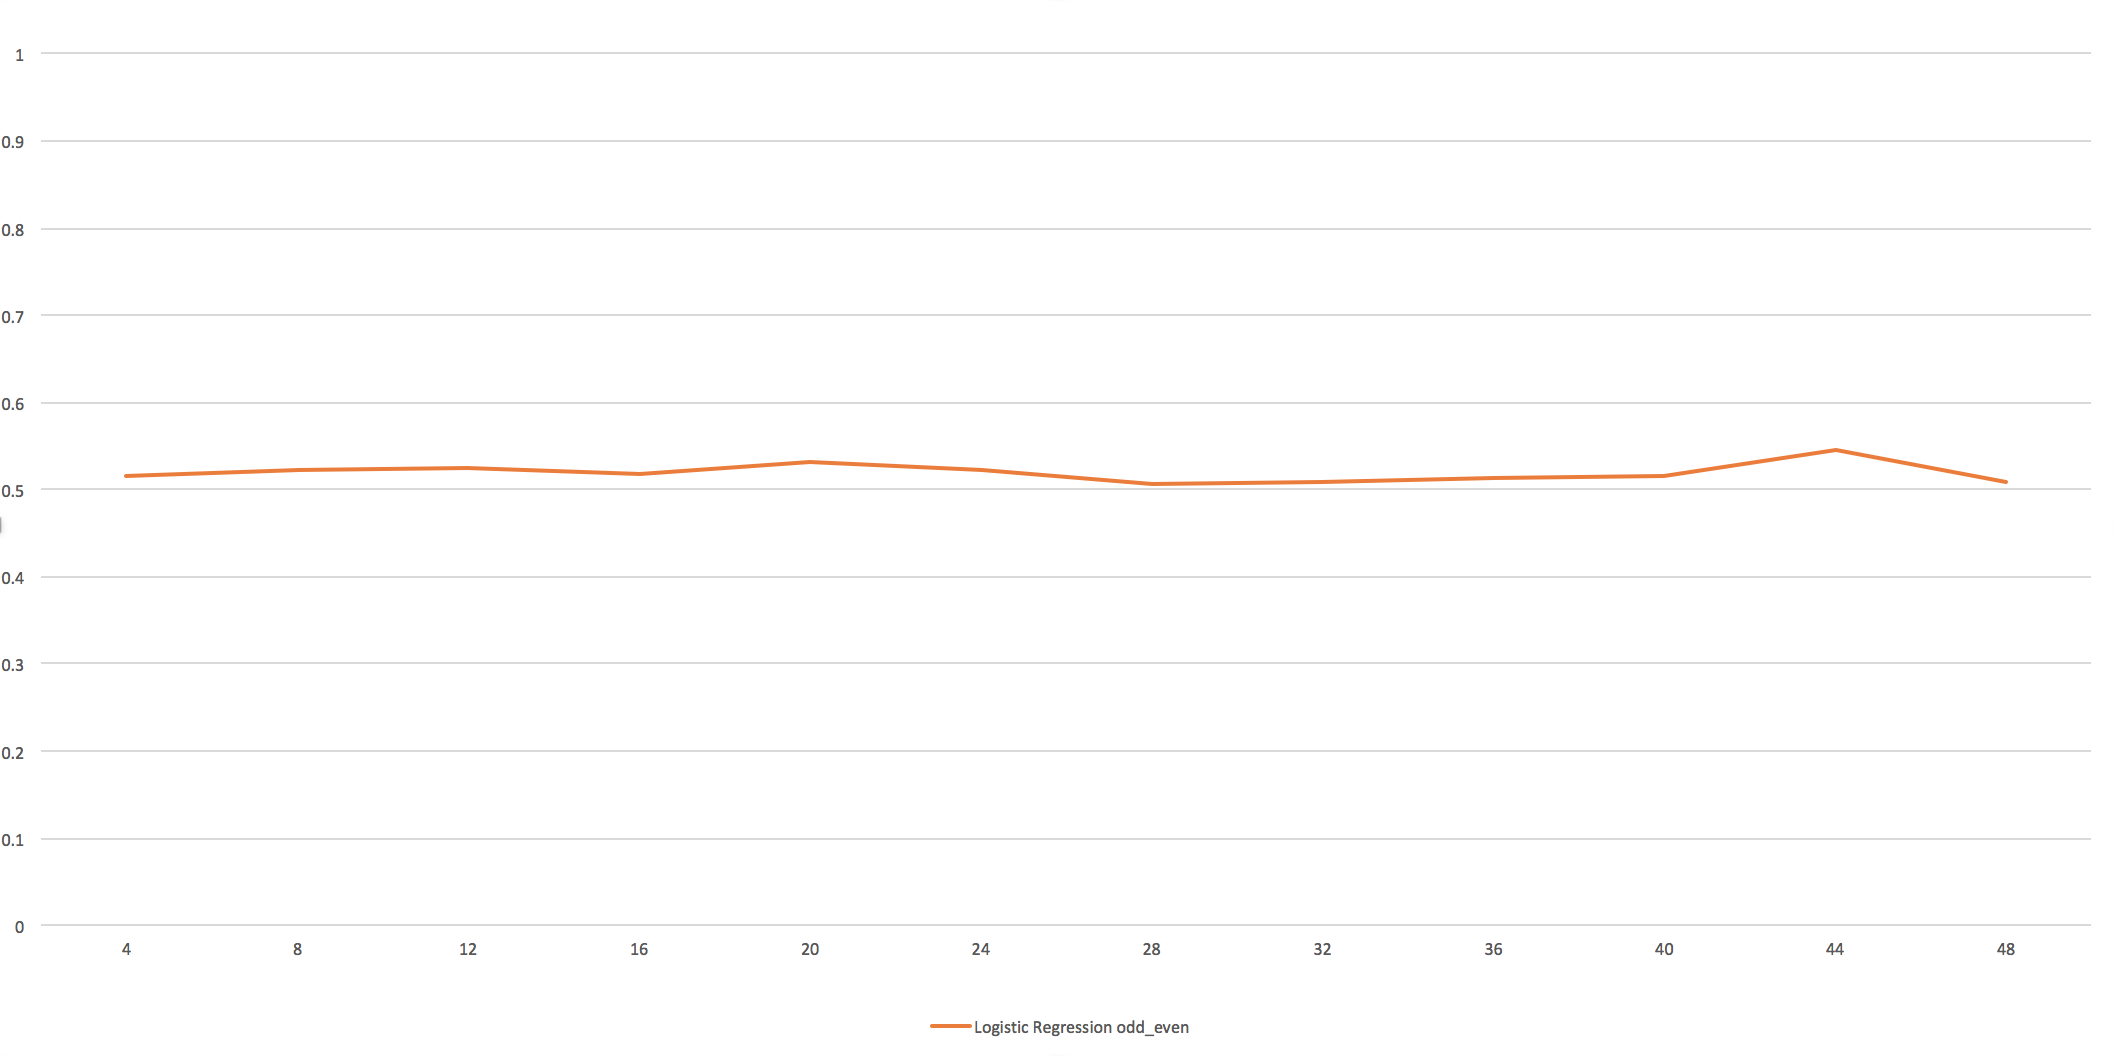
\includegraphics[width=8cm,height=5cm]{images/log_reg_odd_even.png} \\
(в) дали двата тима ќе поентираат & (г) парен/непарен број на голови \\
\end{tabular}
\caption{Резултати од тестирање со логистичка регресија}
\label{fig:log_reg}
\end{figure}

\subsection{Машини со носечки вектори}
Машини со носечки вектори SVM (анг.) \cite{cortes1995support} е можеби еден од најпопуларните алгоритми за машинско учење \cite{lameski2015svm, zdravevski2015robust}.
SVM класифицира податоци со наоѓање на најдобра хиперрамнина која ги одделува сите податоци точки од една класа од оние на другата класа. Најдобра хиперрамнина за SVM значи онаа со најголема маргина меѓу двете класи. Маргината значи максимална ширина на просторот паралелен на хиперпамнината кој нема внатрешни податоци.

На сликa \ref{fig:svm} се прикажани резултатите од тестирањето на сите податочни множества со машини со носечки вектори поделени по класа. Најдобри резултати овој алгоритам постигнува кај множествата 49 и 50 дефинирани во табела \ref{table:datasets}, со 55.19\% за класифицирање на 1 Х 2 игра, односно 67.38\% за класифицирање на 1 или Х2 игра.

\begin{figure}[H]
\centering
\begin{tabular}{cc}
  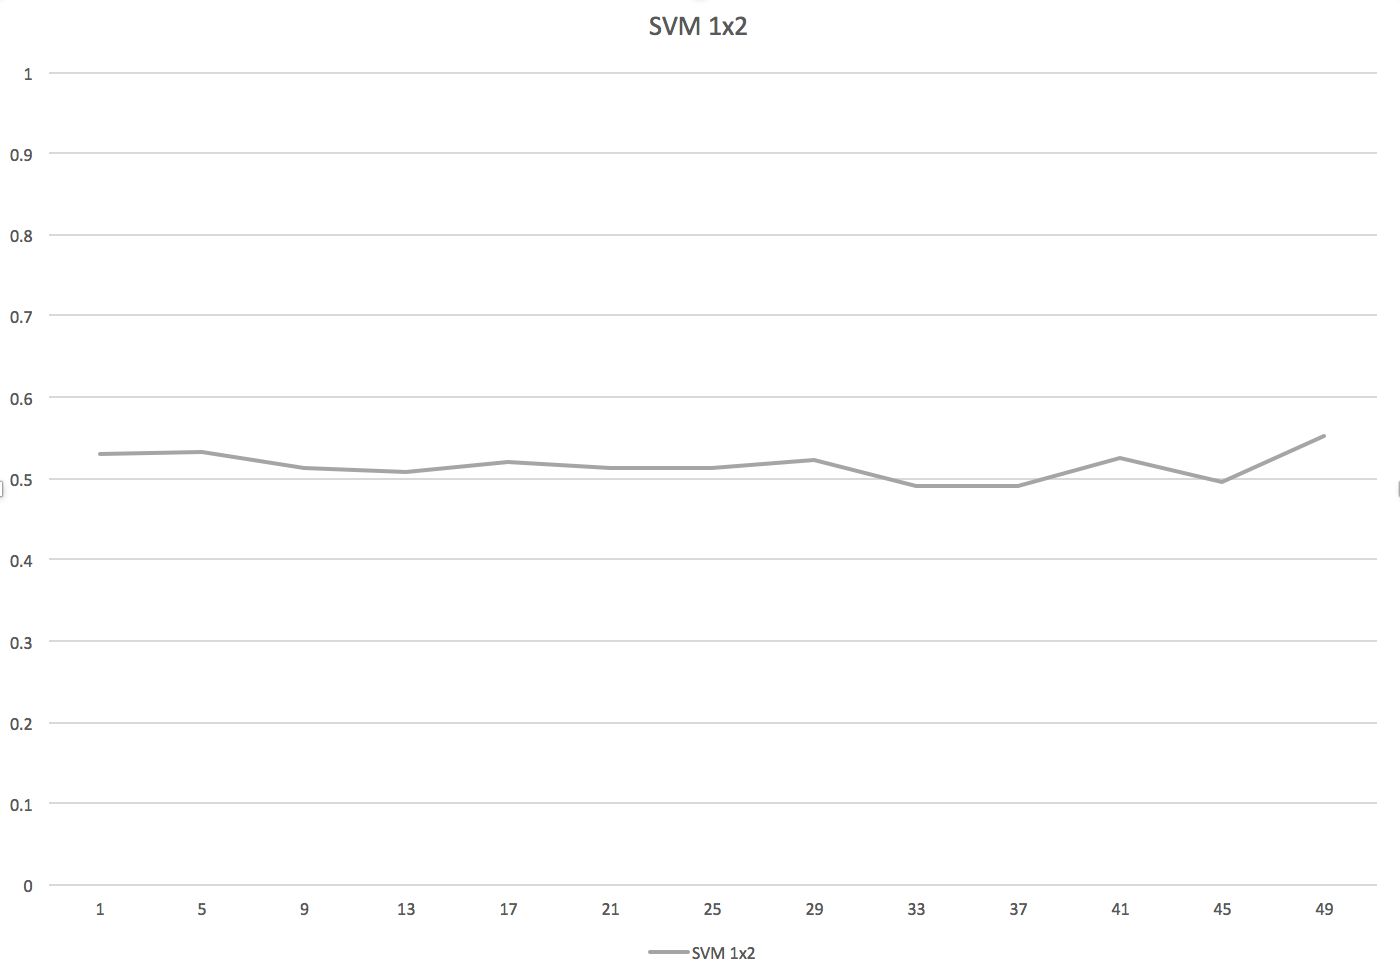
\includegraphics[width=8cm,height=5cm]{images/svm_1x2.png} &   
  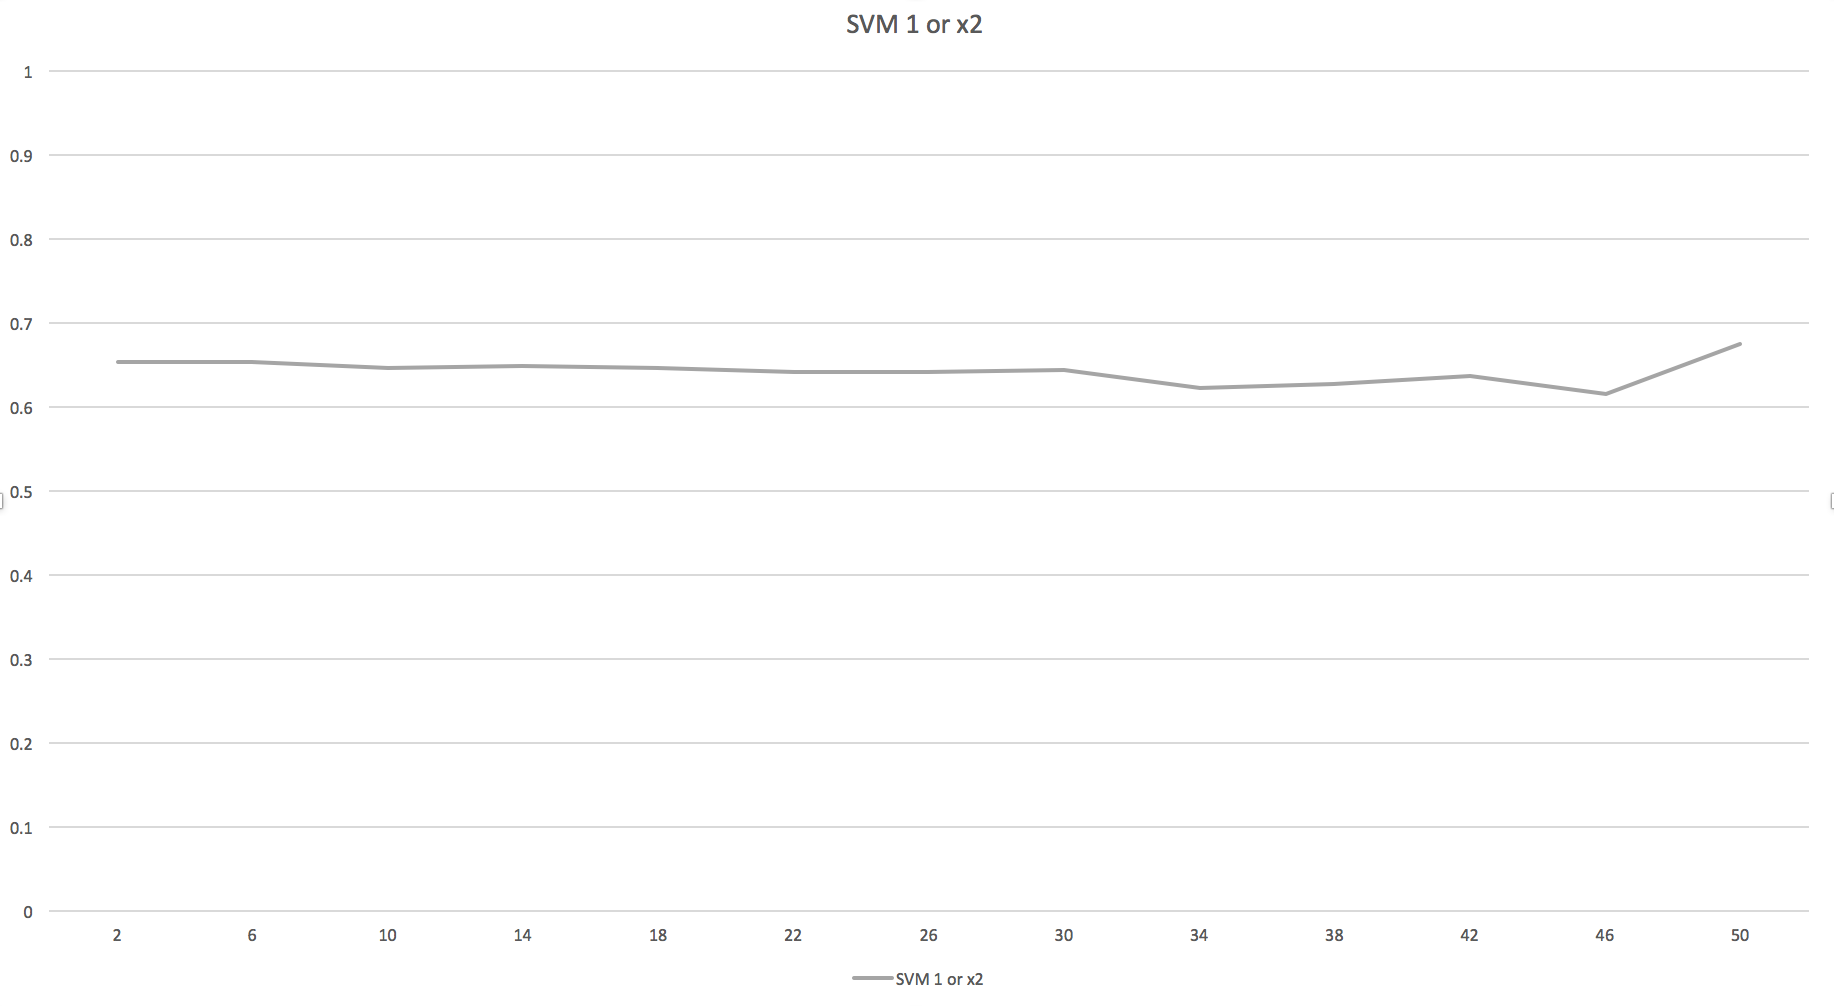
\includegraphics[width=8cm,height=5cm]{images/svm_1_or_x2.png} \\
(а) 1 Х 2 & (б) 1 или Х2 \\
 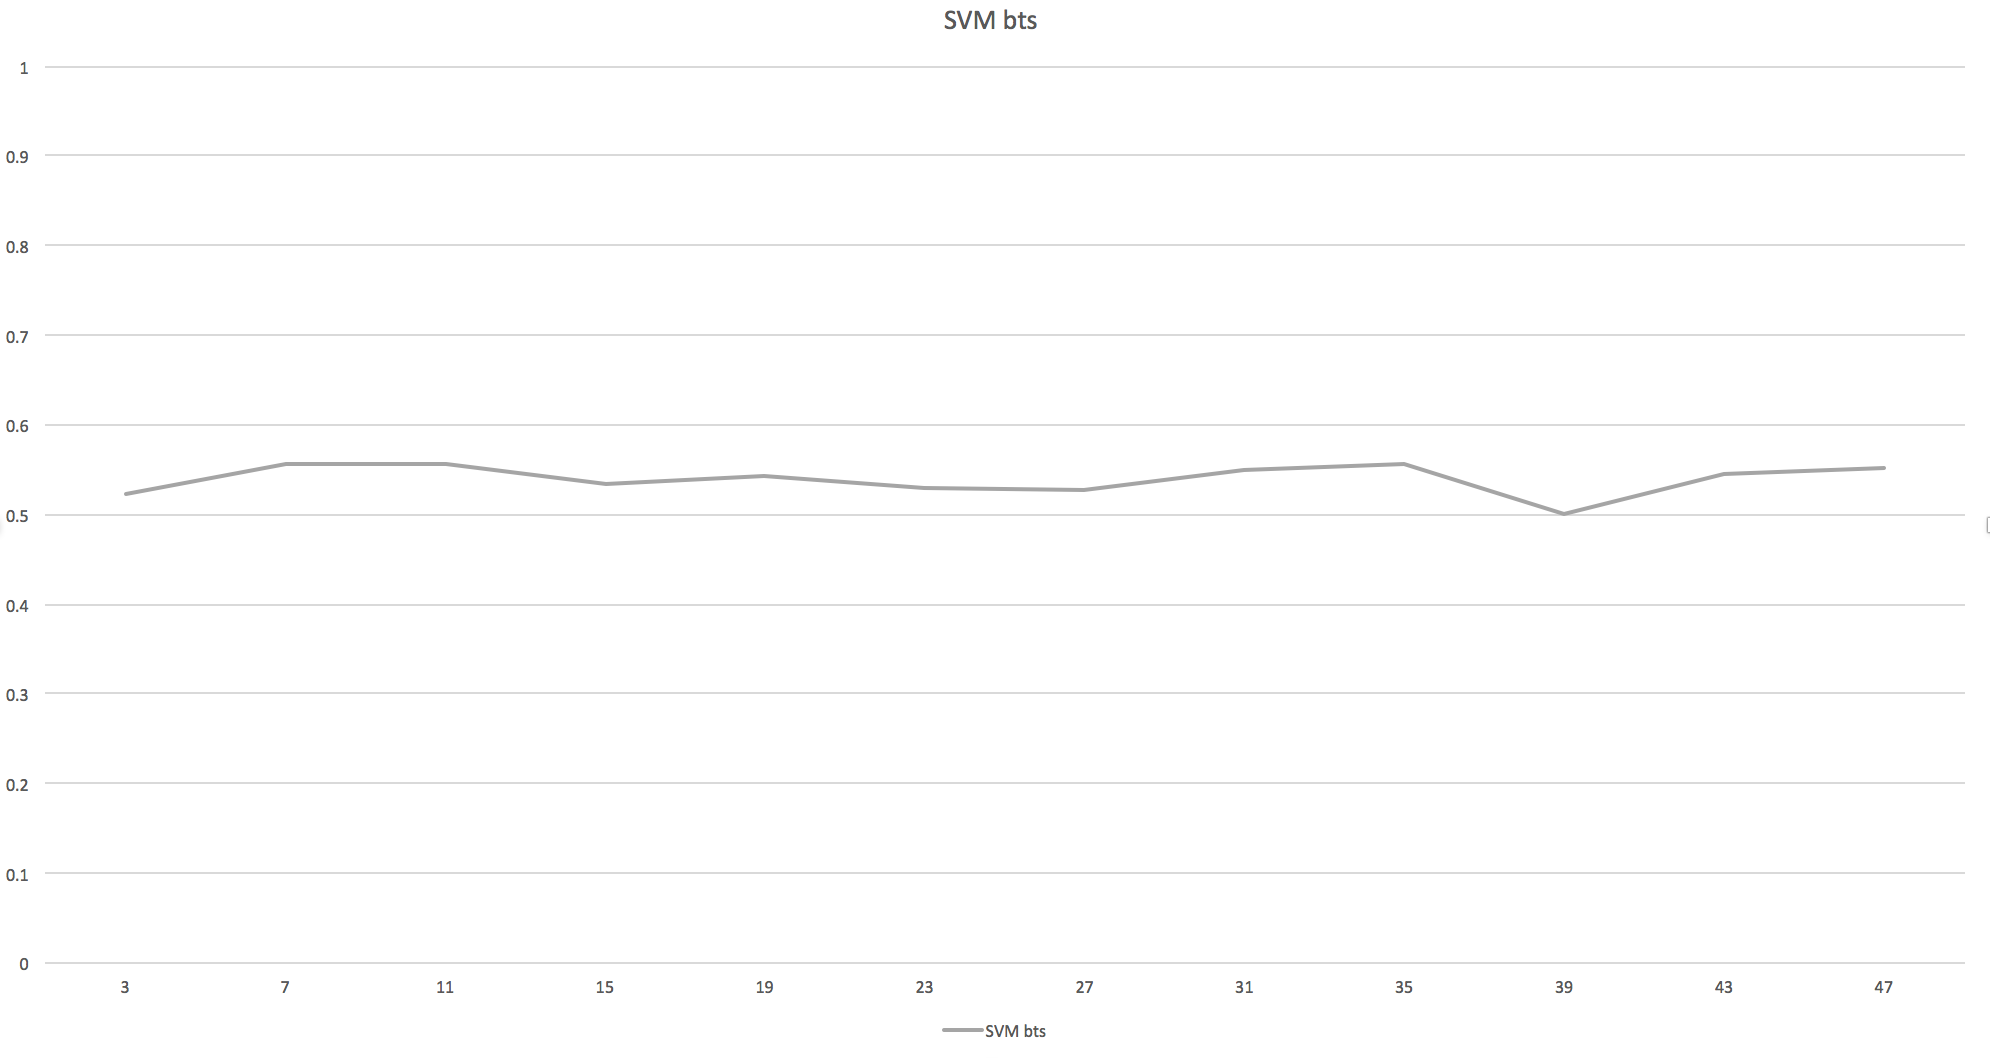
\includegraphics[width=8cm,height=5cm]{images/svm_bts.png}
 &   
 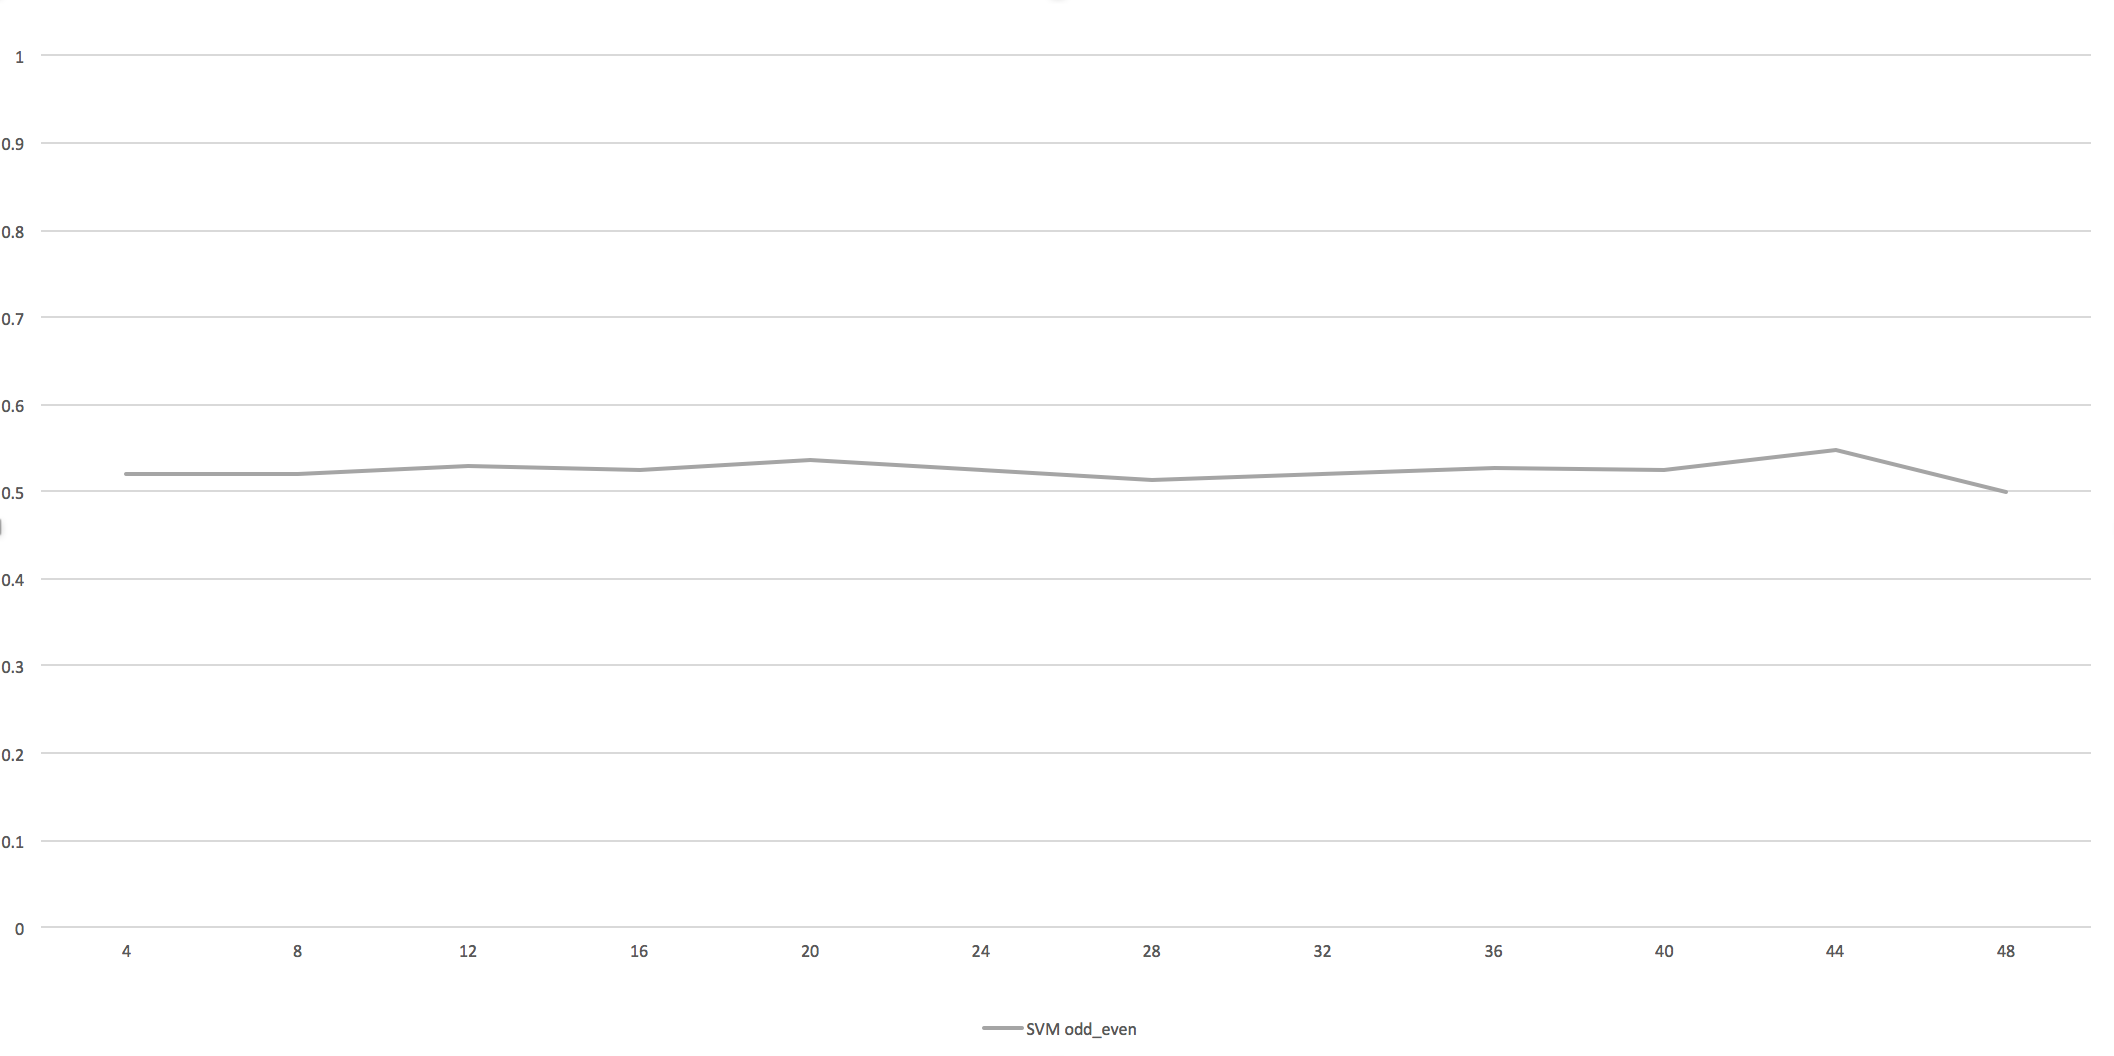
\includegraphics[width=8cm,height=5cm]{images/svm_odd_even.png} \\
(в) дали двата тима ќе поентираат & (г) парен/непарен број на голови \\
\end{tabular}
\caption{Резултати од тестирање со машини со носечки вектори}
\label{fig:svm}
\end{figure}

\subsection{Случаjни шуми}
Случаjни шуми \cite{breiman2001random} е еден од најпопуларните и најмоќните алгоритми за машинско учење. Тоа е еден вид алгоритам за учење на машина за ансамбли, кој комбинира инидивидуални класификатори со цел да се подобрат неговите перформанси.
Во случајни шуми, секое дрво во ансамблот е изградено од примерок составен со замена од сетот за обука. Покрај тоа, при разделување на јазол за време на изградбата на дрвото, поделбата што е избрана повеќе не е најдобрата поделба меѓу сите карактеристики. Наместо тоа, поделбата што е избрана е најдобрата поделба меѓу случајно подмножество на карактеристиките. Како резултат на оваа случајност, пристрасноста на шумата обично малку се зголемува, но, поради просекот, неговата варијанса исто така се намалува, обично повеќе отколку компензирање за зголемување на пристрасноста, оттаму дава севкупен подобар модел.

На сликa \ref{fig:random_forest} се прикажани резултатите од тестирањето на сите податочни множества со случајни шуми поделени по класа. Најдобри резултати овој алгоритам постигнува кај множествата 49, 22 и 50 дефинирани во табела \ref{table:datasets}, со 55.19\% за класифицирање на 1 Х 2 игра, односно 64.57\% и 64.51\% за класифицирање на 1 или Х2 игра.

\begin{figure}[H]
\centering
\begin{tabular}{cc}
  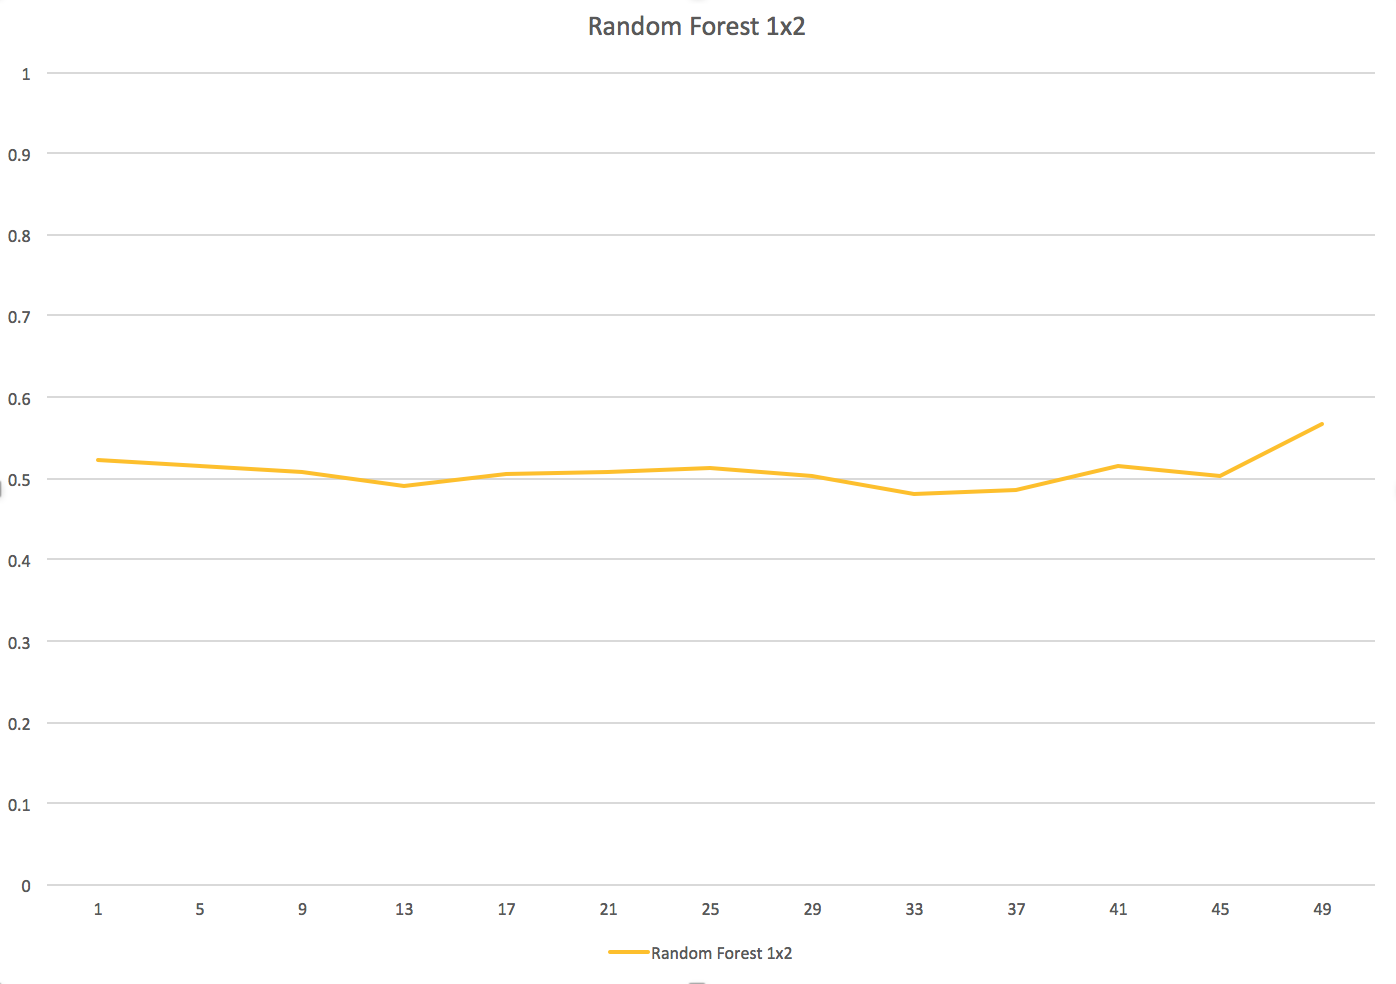
\includegraphics[width=8cm,height=5cm]{images/rf_1x2.png} &   
  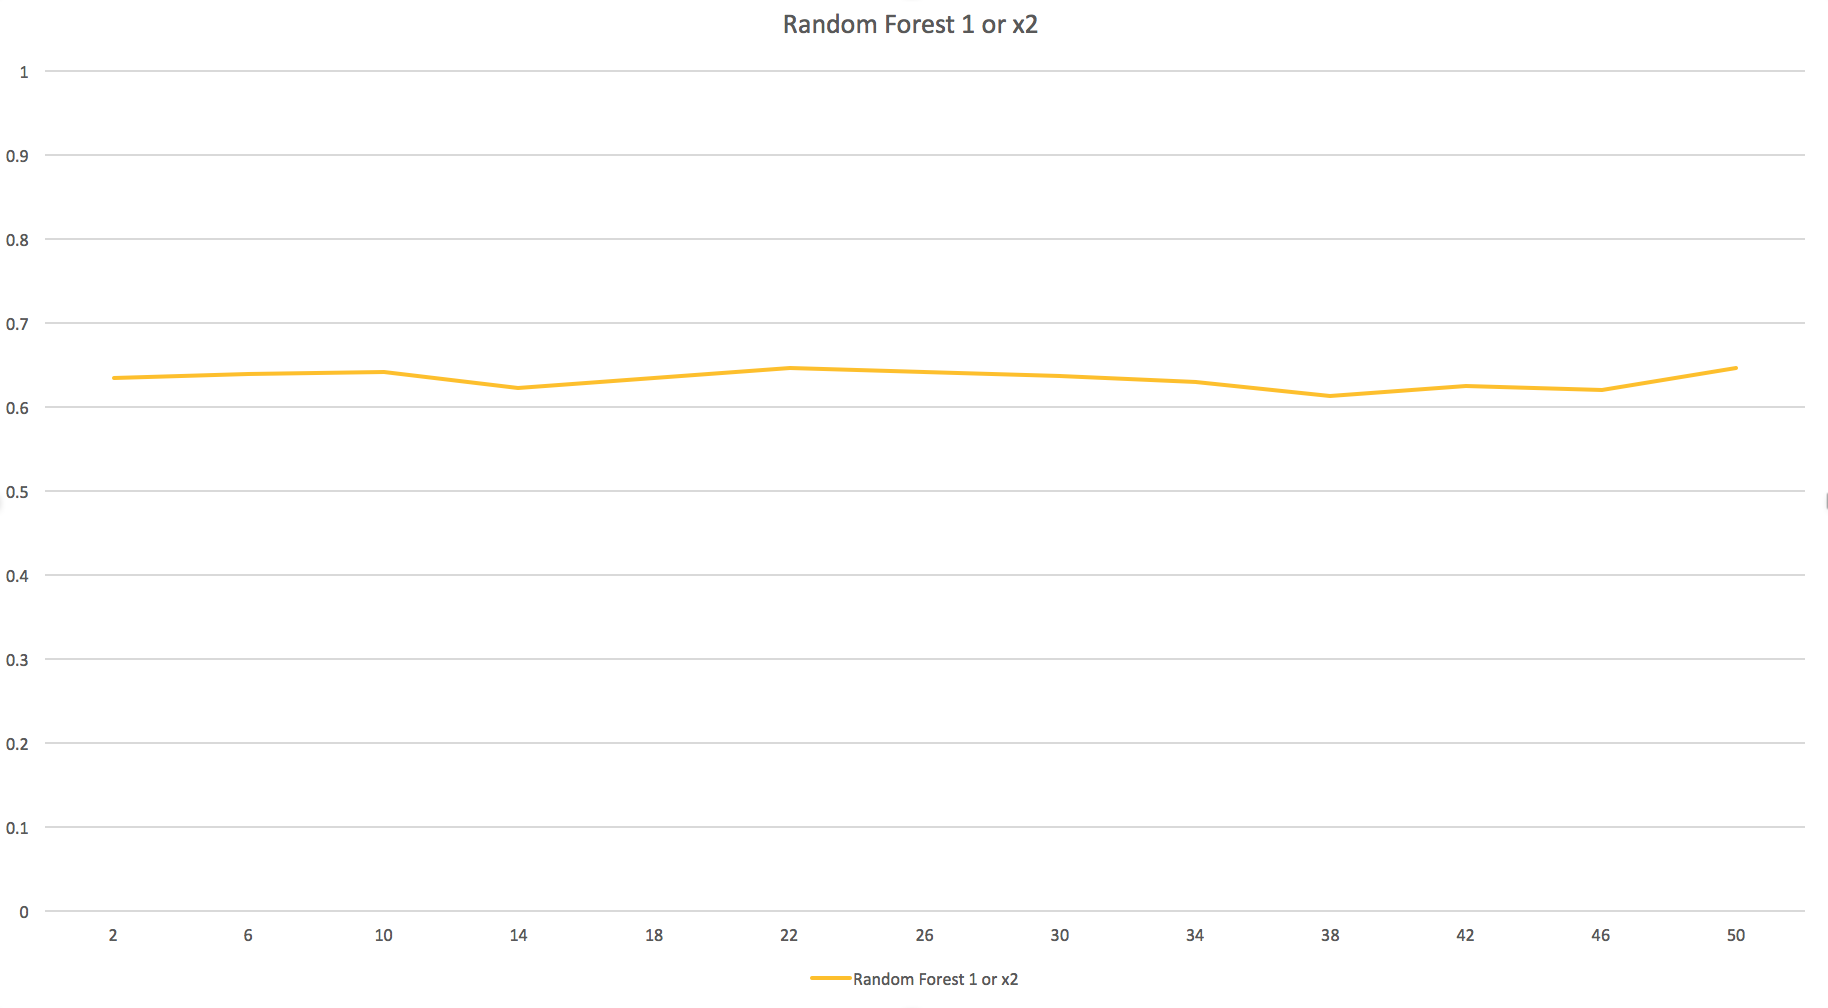
\includegraphics[width=8cm,height=5cm]{images/rf_1_or_x2.png} \\
(а) 1 Х 2 & (б) 1 или Х2 \\
 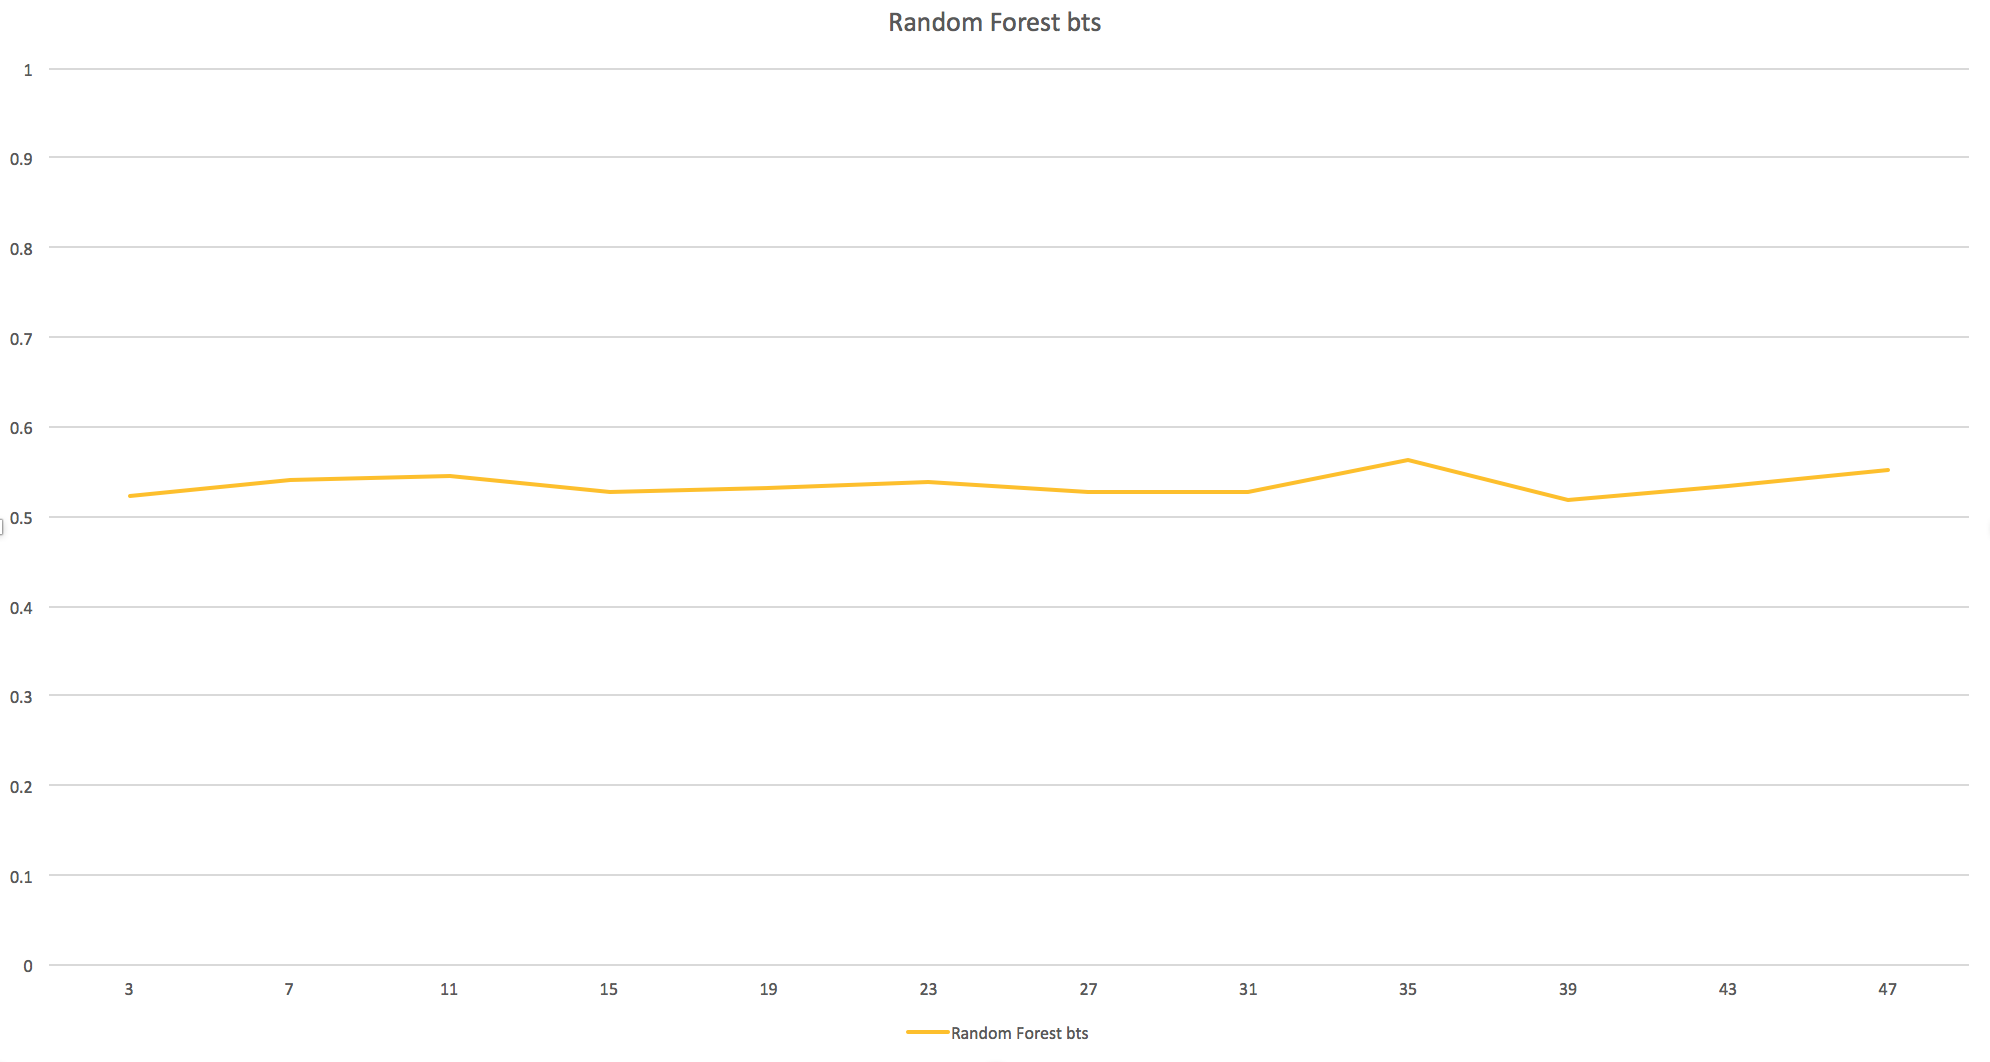
\includegraphics[width=8cm,height=5cm]{images/rf_bts.png}
 &   
 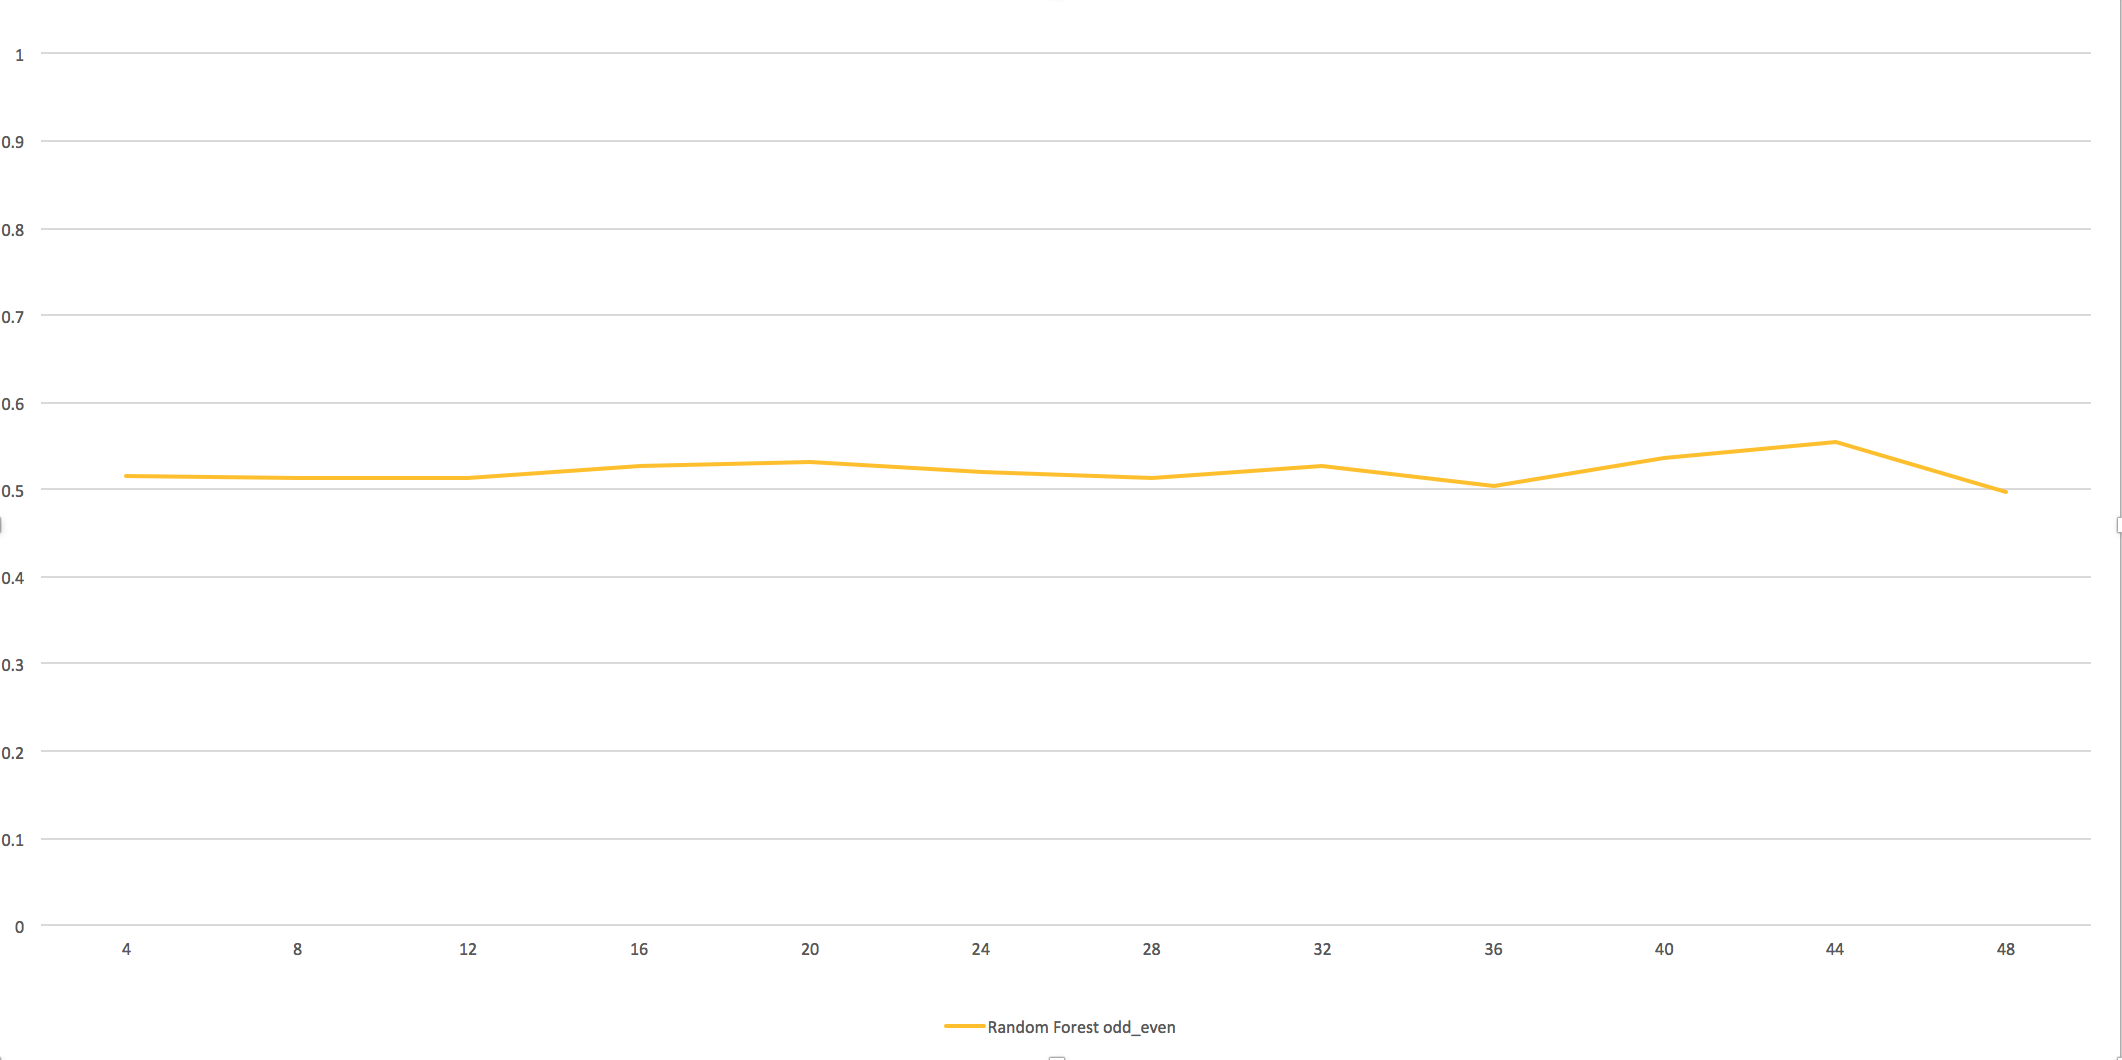
\includegraphics[width=8cm,height=5cm]{images/rf_odd_even.png} \\
(в) дали двата тима ќе поентираат & (г) парен/непарен број на голови \\
\end{tabular}
\caption{Резултати од тестирање со случајни шуми}
\label{fig:random_forest}
\end{figure}

\subsection{Екстремно случаjни дрва}

Во екстремно рандомизирани дрвја \cite{geurts2006extremely}, случајноста оди еден чекор понатаму во начинот на кој се пресметуваат поделбите. Како во случајни шуми, се користи случајно подмножество на карактеристични кандидати, но наместо да се бараат најдискриминирачки прагови, праговите се избираат по случаен избор за секоја кандидатска функција, а најдобриот од овие прагови генерирани по случаен избор се земаат како правило за разделување. Ова обично овозможува малку повеќе да се намали варијансата на моделот, на сметка на малку поголемо зголемување на пристрасноста.

На сликa \ref{fig:ert} се прикажани резултатите од тестирањето на сите податочни множества со екстремно случаjни дрва поделени по класа. Најдобри резултати овој алгоритам постигнува кај множествата 49 и 50 дефинирани во табела \ref{table:datasets}, со 57.7\% за класифицирање на 1 Х 2 игра, односно 66.67\% за класифицирање на 1 или Х2 игра.

\begin{figure}[H]
\centering
\begin{tabular}{cc}
  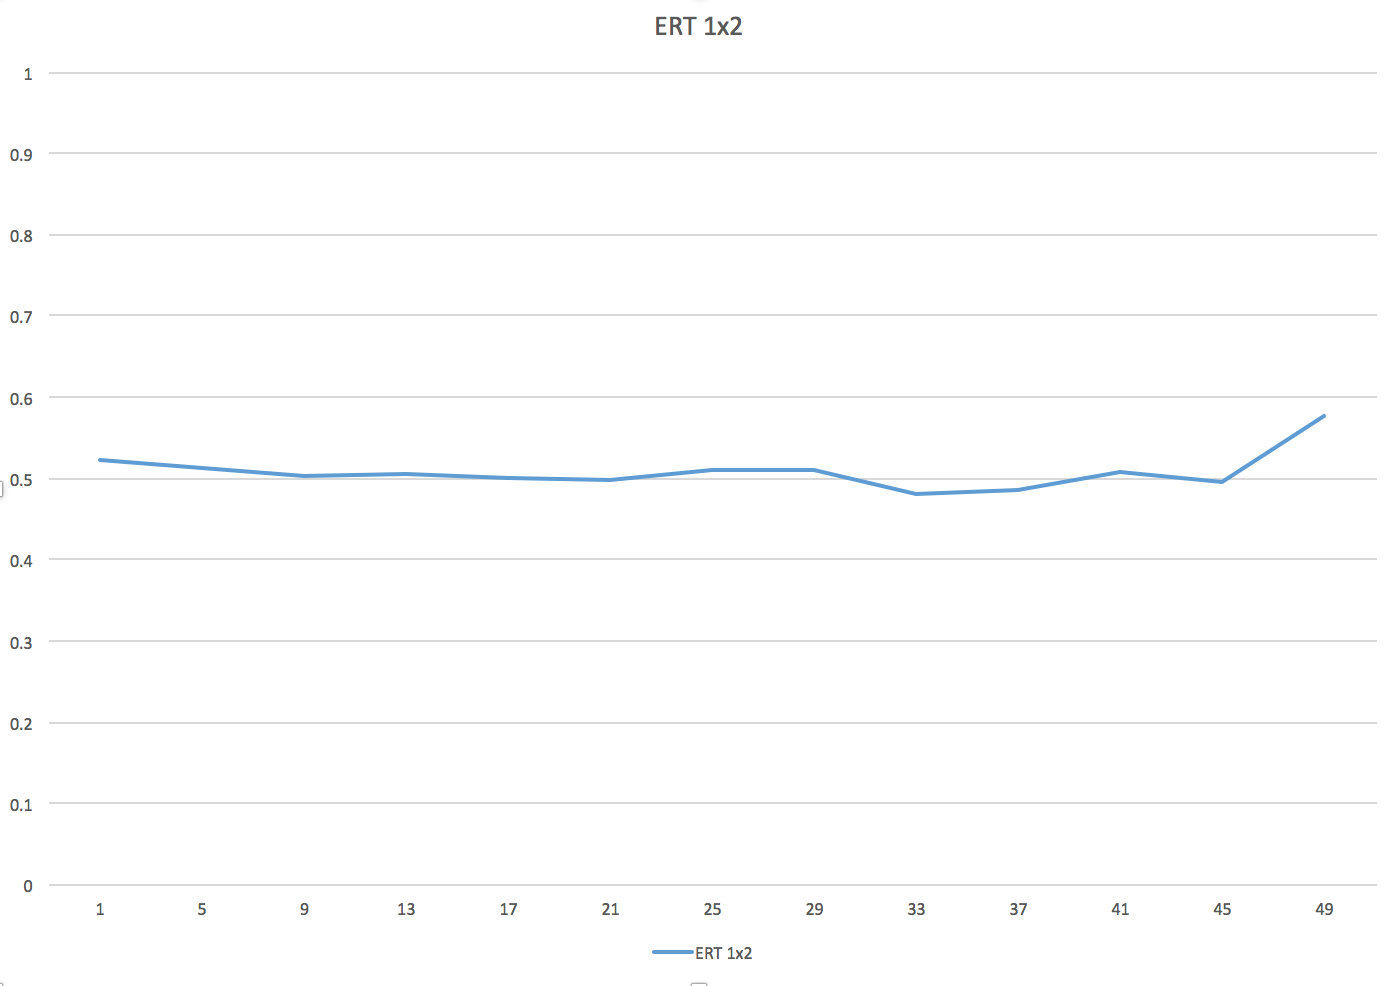
\includegraphics[width=8cm,height=5cm]{images/ert_1x2.png} &   
  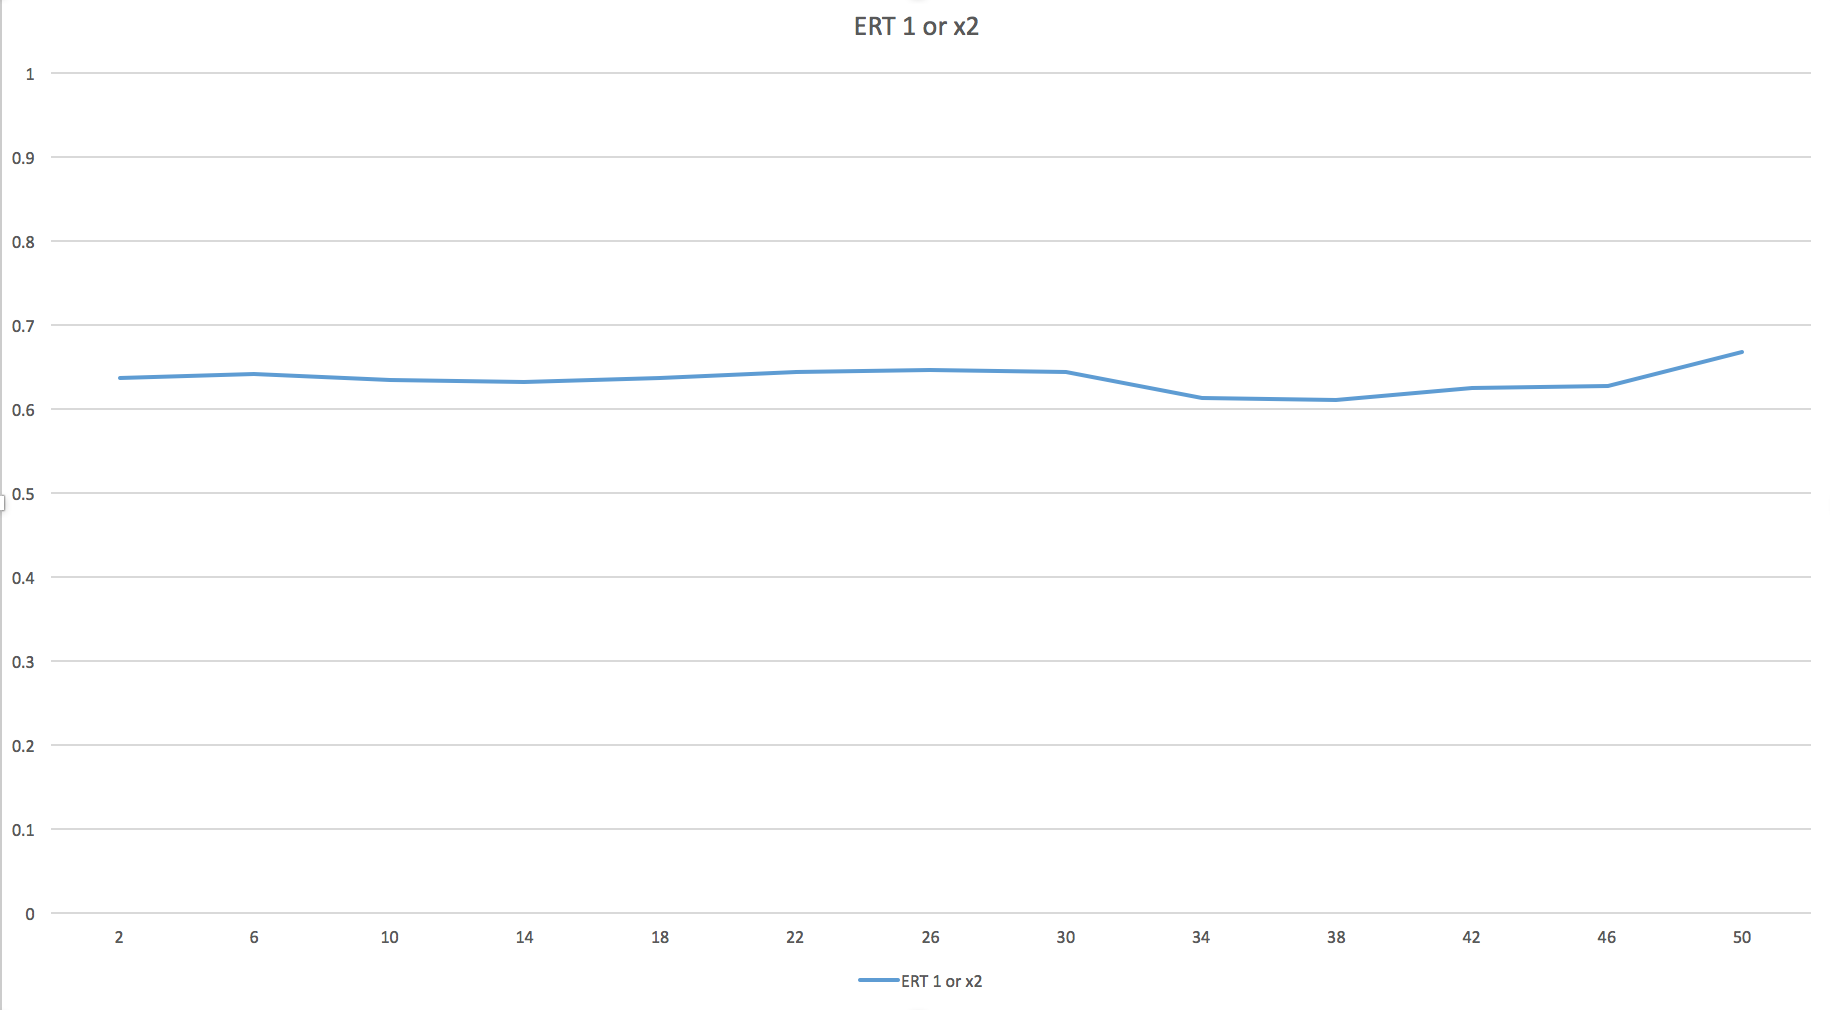
\includegraphics[width=8cm,height=5cm]{images/ert_1_or_x2.png} \\
(а) 1 Х 2 & (б) 1 или Х2 \\
 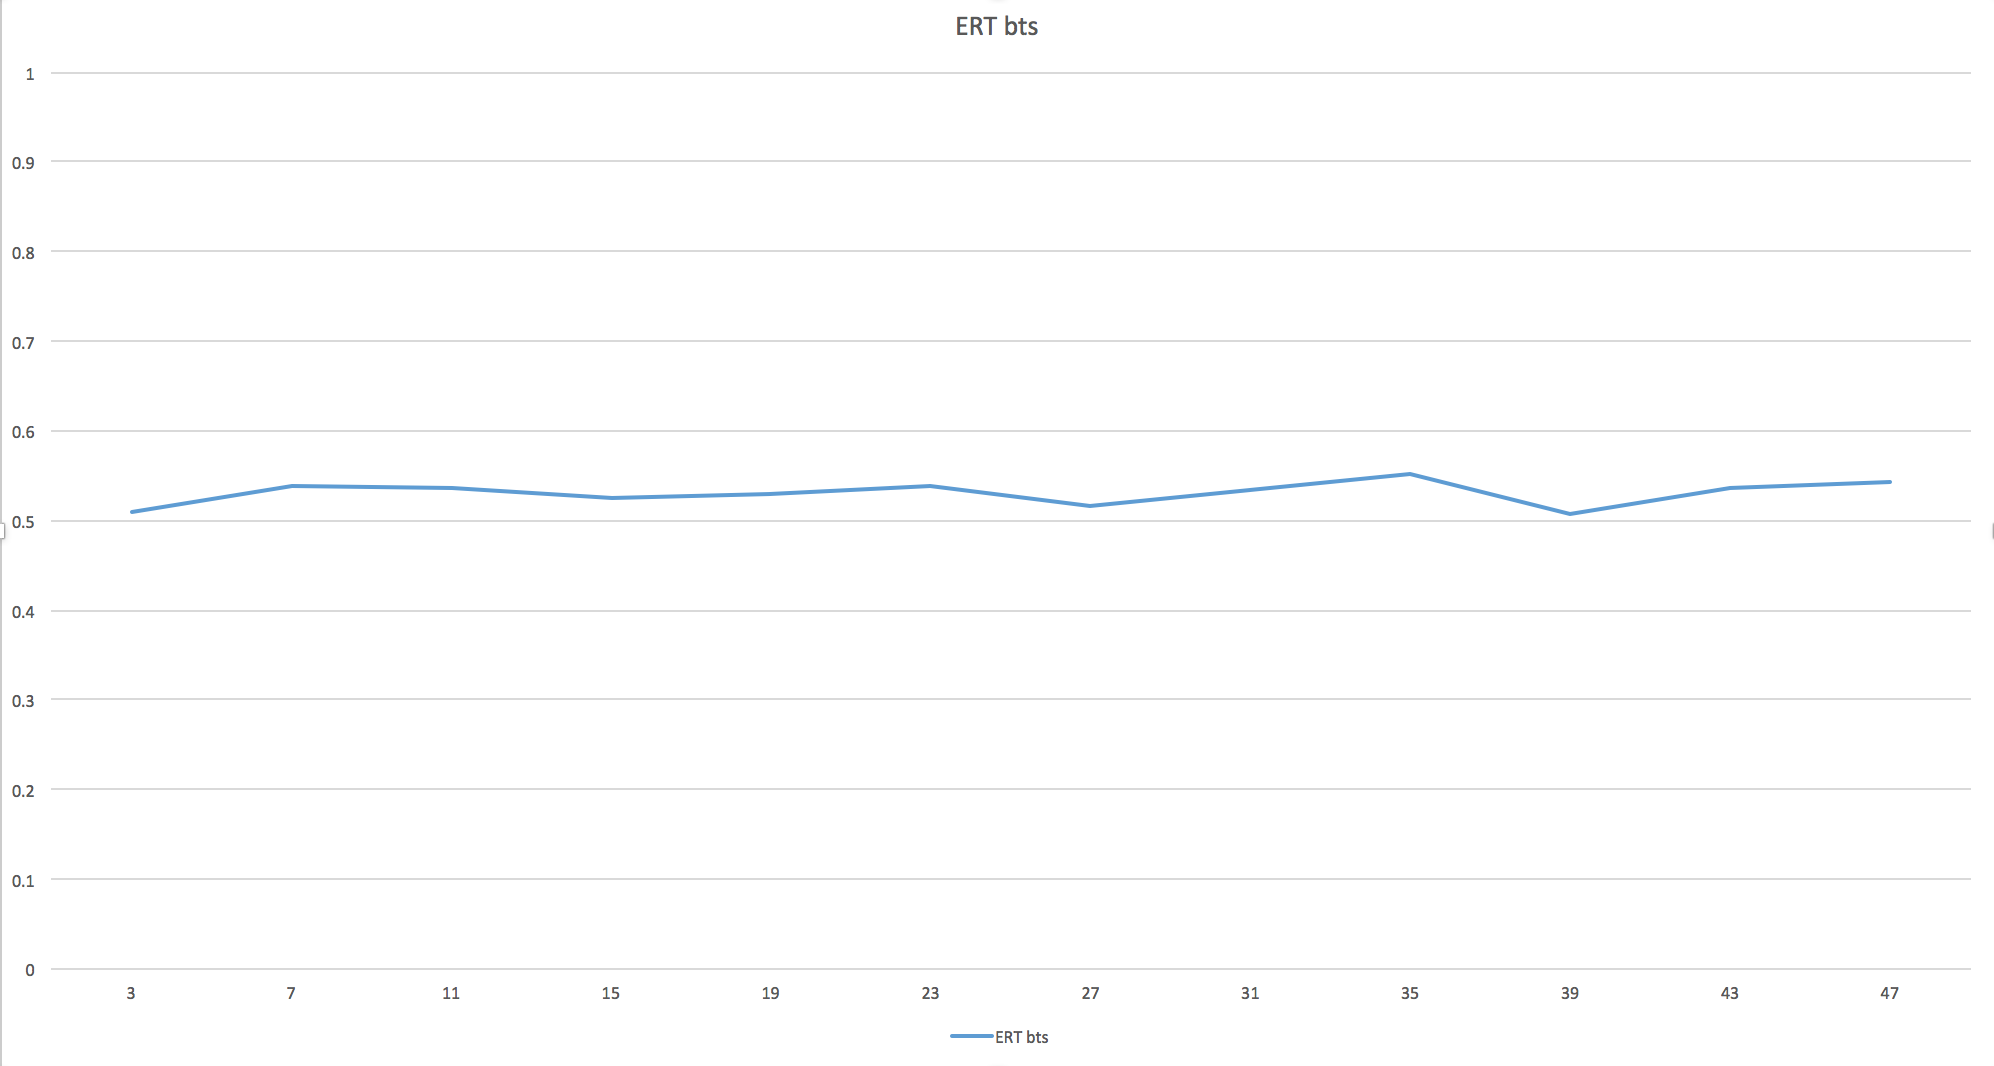
\includegraphics[width=8cm,height=5cm]{images/ert_bts.png}
 &   
 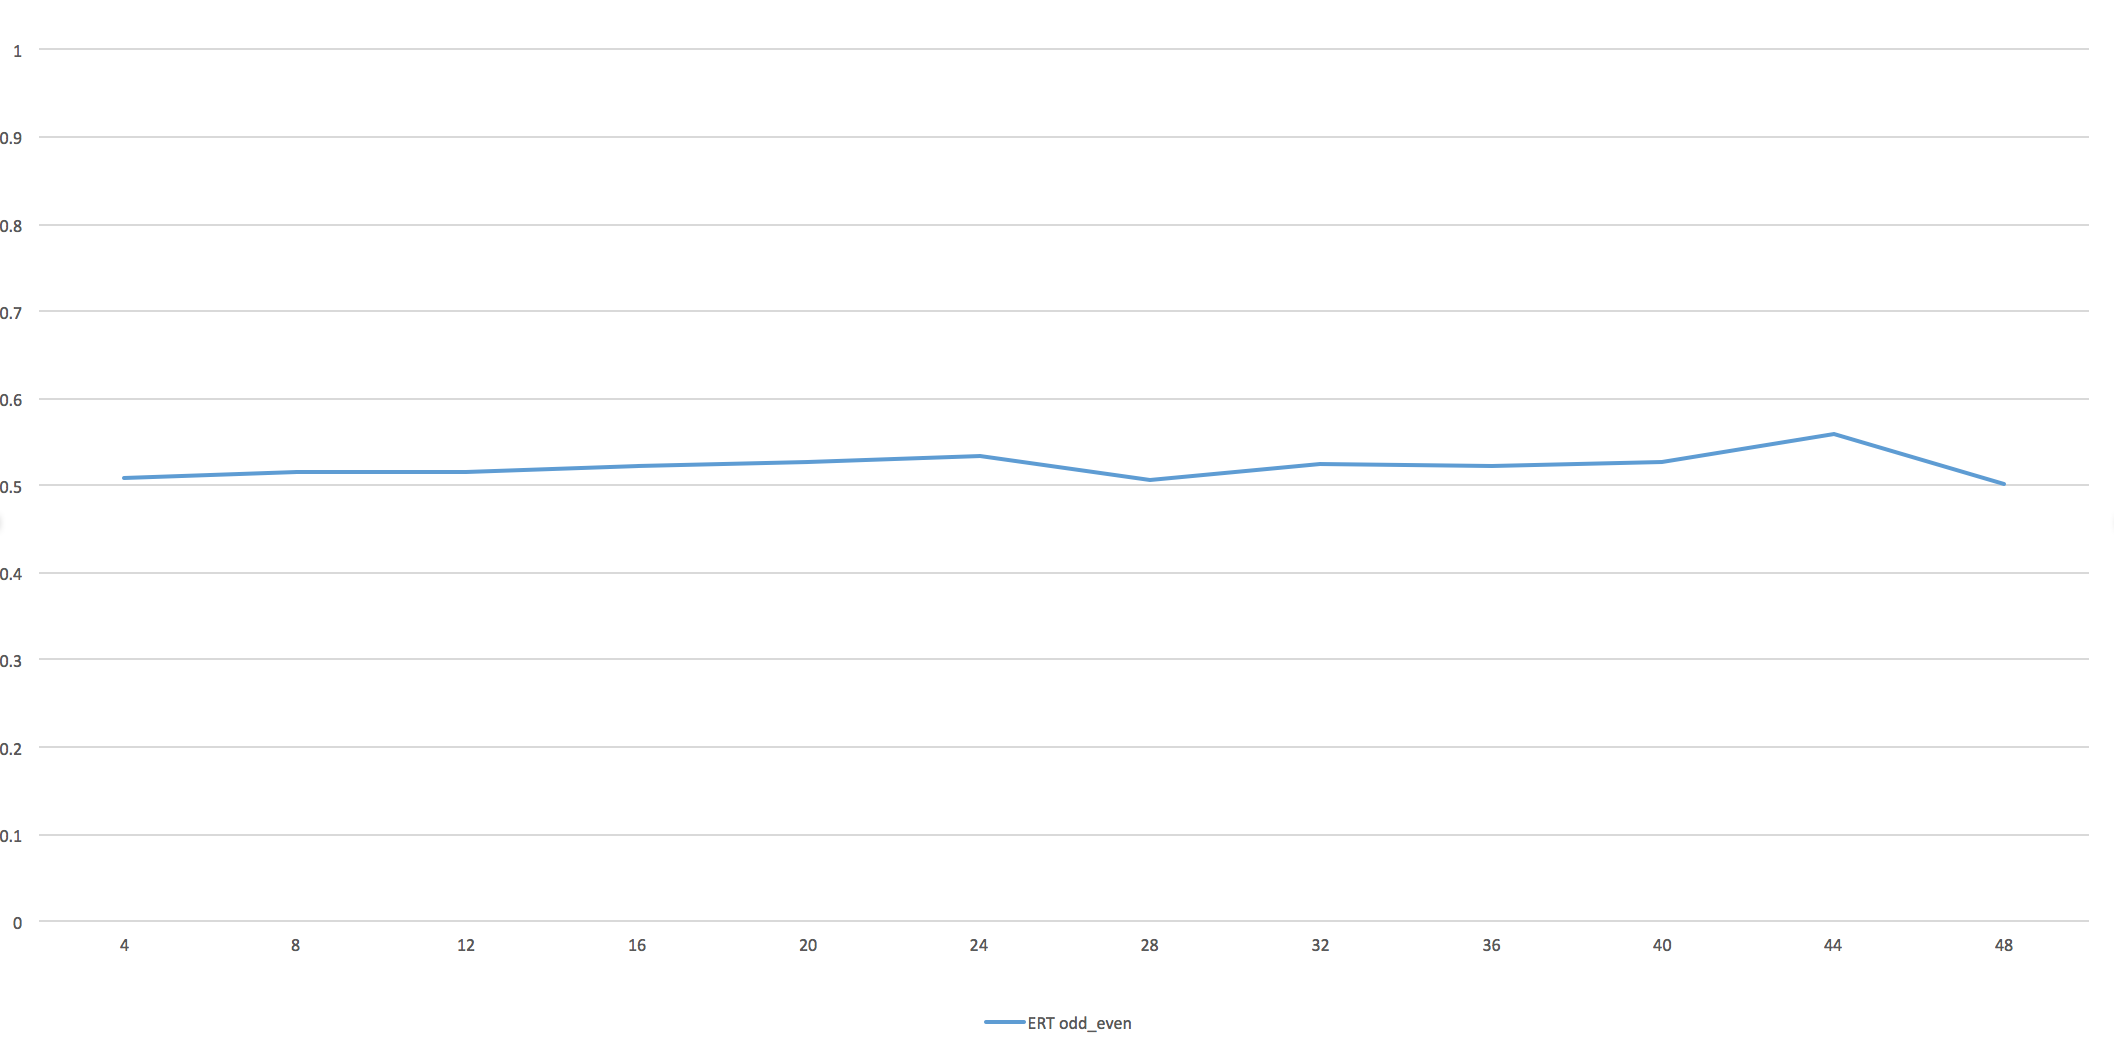
\includegraphics[width=8cm,height=5cm]{images/ert_odd_even.png} \\
(в) дали двата тима ќе поентираат & (г) парен/непарен број на голови \\
\end{tabular}
\caption{Резултати од тестирање со екстремно случаjни дрва}
\label{fig:ert}
\end{figure}


\section{Вештачки невронски мрежи}
Полето на вештачките невронски мрежи \cite{schalkoff1997artificial} честопати се нарекуваат и само невронски мрежи, истражува како едноставни модели на биолошки мозоци може да се искористат за решавање на тешките пресметковни задачи како што се задачите за предвидувачко моделирање што ги гледаме во машинско учење. Целта не е да се создадат реални модели на мозокот, туку да се развијат робустен алгоритми и структури на податоци кои можеме да ги користиме за моделирање на тешки проблеми.
Моќта на невронските мрежи доаѓа од нивната способност да ја научат застапеноста во податоците за обука и како најдобро да се поврзат со излезната променлива што сакаме да ја предвидиме. Во оваа смисла, невронските мрежи учат мапирање. Математички, тие се способни да научат која било функција за мапирање и се докажа дека е универзален апроксимациски алгоритам.
Предвидувачката способност на невронските мрежи доаѓа од хиерархиската или повеќеслојна структура на мрежите. Структурата на податоци може да ги одбере, научи да ги претставува, функциите на различни размери или резолуции и да ги комбинира во функции со повисок редослед. На пример од линии, до збирки на линии до форми.

Основната градежна единка за невронските мрежи се вештачки неврони.
Ова се едноставни пресметковни единици кои имаат пондерирани влезни сигнали и произведуваат излезен сигнал со користење на функцијата за активирање.

Пондерираните влезови се сумираат и пренесуваат преку функцијата за активација, понекогаш наречена функција за трансфер.
Функцијата за активација е едноставно мапирање на сумиран пондериран влез на излезот на невронот. Таа се нарекува функција за активација, бидејќи го регулира прагот на активирање на невронот и сила на излезниот сигнал.
Традиционално се користат нелинеарни функции за активирање. Ова и овозможува на мрежата да ги комбинира влезовите на покомплексни начини и, за возврат, обезбедува побогата можност во функциите што може да ги моделираат. Нелинеарните функции како што е логистичката, исто така наречена сигмоидна функција, се користат за да се изведе вредност помеѓу 0 и 1 со дистрибуција во форма на S (лат.), и хиперболичната тангентна функција, која ја дава истата распределба но во опсегот од -1 до +1 .
Во последно време функцијата за активација на исправувачот е покажана за да обезбеди подобри резултати.

Невроните се наредени во мрежи на неврони.
Редот на невроните се нарекува слој и една мрежа може да има повеќе слоеви. Архитектурата на невроните во мрежата често се нарекува мрежна топологија.

Долниот слој што го зема влезот од вашата група на податоци се нарекува видлив слој, бидејќи е изложениот дел од мрежата. Често, невронската мрежа е нацртана со видлив слој со еден неврон по влезна вредност или колона во вашиот назив на податоци. Овие не се неврони како што е опишано погоре, туку едноставно ја пренесуваат влезната вредност иако на следниот слој.

Слоевите по влезниот слој се нарекуваат скриени слоеви, бидејќи тие не се директно изложени на влезот. Наједноставната мрежна структура е да има еден неврон во скриениот слој кој директно ја дава вредноста.
Со оглед на зголемувањето на компјутерската моќ и ефикасните библиотеки, може да се конструираат многу длабоки невронски мрежи. Длабоко учење може да се однесува на тоа да имате многу скриени слоеви во вашата невронска мрежа. Тие се длабоки, бидејќи тие би биле незамисливо бавно да тренираат историски, но може да потрае неколку секунди или минути ако се обучат со користење на современи техники и хардвер.

Последниот скриен слој се нарекува излезен слој и е одговорен за изнесување на вредност или вектор на вредности кои одговараат на формат потребен за проблемот. 

\subsection{Густо поврзани невронски мрежи}

Од експериментите со претходните алгоритми за машинско учење забележавме дека две податочни множества постојано ни даваа најдобри резултати во однос на останатите. Множествата 49 и 50 дефинирани според табела \ref{table:datasets} всушност ги имаат истите атрибути и истата сегментација, но со различни класи. Во овие две множества се земани само натпреварите од англиската премиер лига и секој тим има одиграно ист број натпревари како останатите тимови во множеството. За таа цел одлучивме да го продолжиме нашето истражување само со овие податочни множества. 

За развојот на моделите на невронските мрежи користевме користевме минималистичка библиотека Керас (Keras анг.) напишана во Python програмскиот јазик и може да работи со помош на Theano или TensorFlow. Во Керас постојат повеќе имплементации на невронски мрежи како што се рекурентни невронски мрежи или конволуциски невронски мрежи, но во нашиот случај ние користиме густо поврзани невронски мрежи или целосно поврзани невронски мрежи. Архитектурата на густо поврзаните невронски мрежи е направена така што секој јазол од претходниот слој е поврзан со секој јазол од следниот слој. Проблемот кој го решаваме е претставен како функциско мапирање и овој тип на архитектура е соодветен за вакви проблеми.

Причината зашто невронските мрежи се толку тешки да се конфигурираат е бидејќи постојат многу параметри кои треба да се постават. Во нашиот случај за наѓање на соодветните параметри, применивме техники на пребарување како во \cite{lameski2015svm}. Во табела \ref{table:params} се прикажани параметрите за кои пребарувавме и нивниот опис. 

\begin{table}[hbtp]
 \centering
 \scalebox{0.45}{%
 \begin{tabular}{| c | c |}
 \hline
 параметар & опис \\ 
 \hline
 \hline
 batch\_size & бројот на инстанци кои се оценуваат пред да се изврши ажурирање на тежината во мрежата \\ 
 \hline
 epochs & број на итерации во еден тренинг процес \\ 
 \hline
 dropout & случајно поставување фракција на влезни единици на 0 во секое ажурирање за време на обуката, што помага да се спречи претренирање (overfitting, анг.) \\ 
 \hline
 kernel\_constraint & функцијата за ограничување се применува на матрицата на тежини \\ 
 \hline
 neurons & број на неврони во скриениот слој \\ 
 \hline
  activation & активациска функција \\ 
 \hline
 optimizer & оптимизациски алгоритам \\ 
 \hline
 loss & вредност што ние се обидуваме да ја минимизираме за време на нашата обука на моделот \\ 
 \hline
\end{tabular}}
\caption{Параметри за конфигурација на модел на невронски мрежи во Керас}
\label{table:params}
\end{table}
За скриените слоеви ја користевме 'relu' (rectified linear unit) активациската функција како параметар за активација, додека во излезниот слој користевме сигмоидна функција 'sigmoid'. 
Ја користиме сигмоидната функција на излезниот слој за да осигуриме дека нашата излезна мрежа е помеѓу 0 и 1 и лесно може да се мапира или на веројатност од 0 до 1 или припрема на класификација на било која класа со стандарден праг од 0,5. Како оптимизациски алгоритам го користиме 'adam' \cite{kingma2014adam}. За 'loss' параметарот како вредности кои треба да ги минимизираме за множеството 49 користевме 'categorical\_crossentropy' бидејќи овде имаме 3 класи (1 Х 2) и излезниот слој ќе содржи 3 неврони, додека за множеството 50 користевме 'binary\_crossentropy' бидејќи во ова множество се само 2 класи (1 или Х2) и излезниот слој може да се претстави само со 1 неврон. Oстанатите параметри ги добивме со пребарување и оптимизација.

\begin{table}[hbtp]
 \centering
 \scalebox{0.7}{%
 \begin{tabular}{| c | c |}
 \hline
 параметар & вредности \\ 
 \hline
 \hline
 batch\_size & 20, 32, 64\\ 
 \hline
 epochs & 50, 80, 120 \\ 
 \hline
 dropout & 0.2, 0.5, 0.8 \\ 
 \hline
 kernel\_constraint & 4, 6, 8 \\ 
 \hline
 hidden\_layers & 1, 2, 3, 4 \\
  \hline
 neurons &  (влезна димезнија)/4, (влезна димензија)/2, (влезна димензија)*1, (влезна димензија)*2 \\ 
 \hline
\end{tabular}}
\caption{Вредности на хипер-параметрите користени за пребарување и оптимизација на моделот}
\label{table:params_grid}
\end{table}

Пребарувањето на параметрите го вршевме со тренирање на тренинг множеството и тестиравме врз валидациското множество. По извршеното пребарување низ вредностите на параметрите прикажани во табела \ref{table:params_grid}, добивме оптимална конфигурација на моделот со параметри прикажани во табела \ref{table:params_conf_49} и табела  \ref{table:params_conf_50}. Резултатите од пребарувањето се прикажани на слика \ref{fig:grid_search_49} и слика  \ref{fig:grid_search_50}.

\begin{figure}[hbtp]
\centering
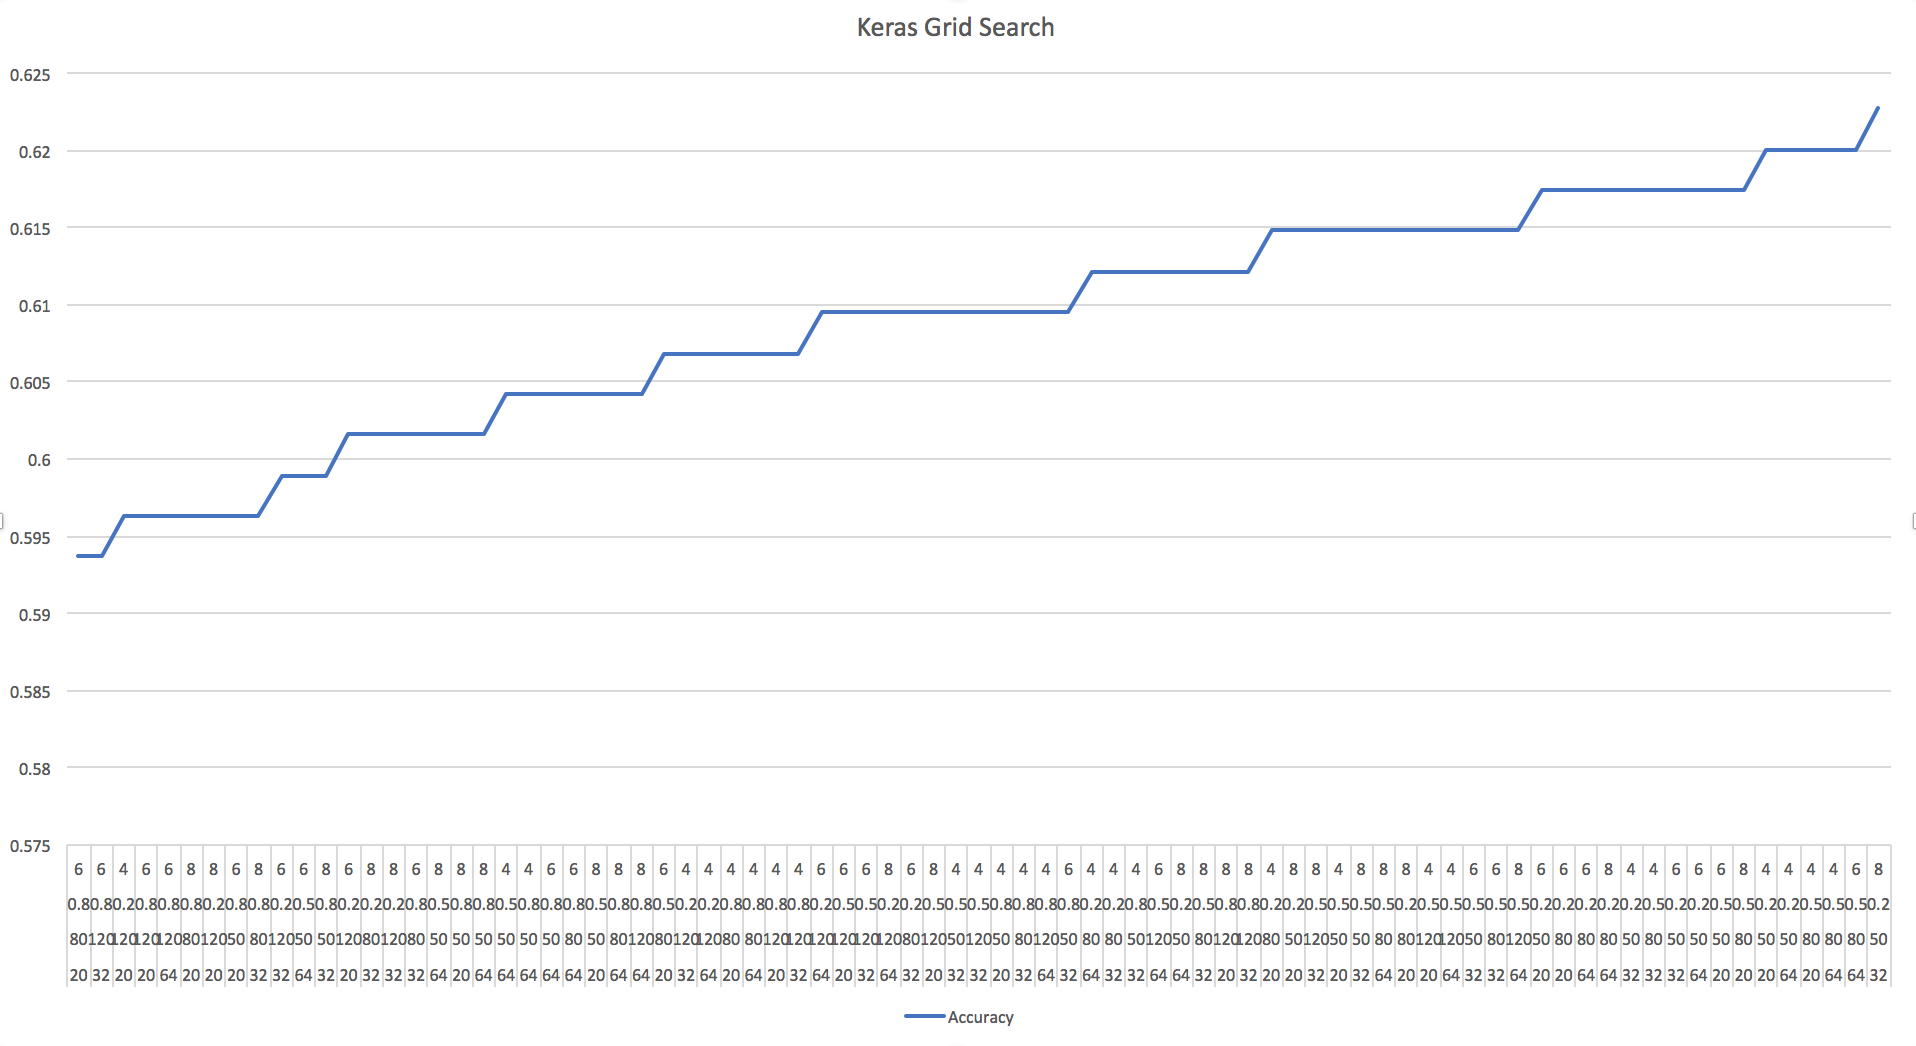
\includegraphics[width=14cm,height=8cm]{images/keras_grid_search.png}
\caption{Оптимизација на моделот преку пребарување за множество 49}
\label{fig:grid_search_49}
\centering
\end{figure}

\begin{figure}[hbtp]
\centering
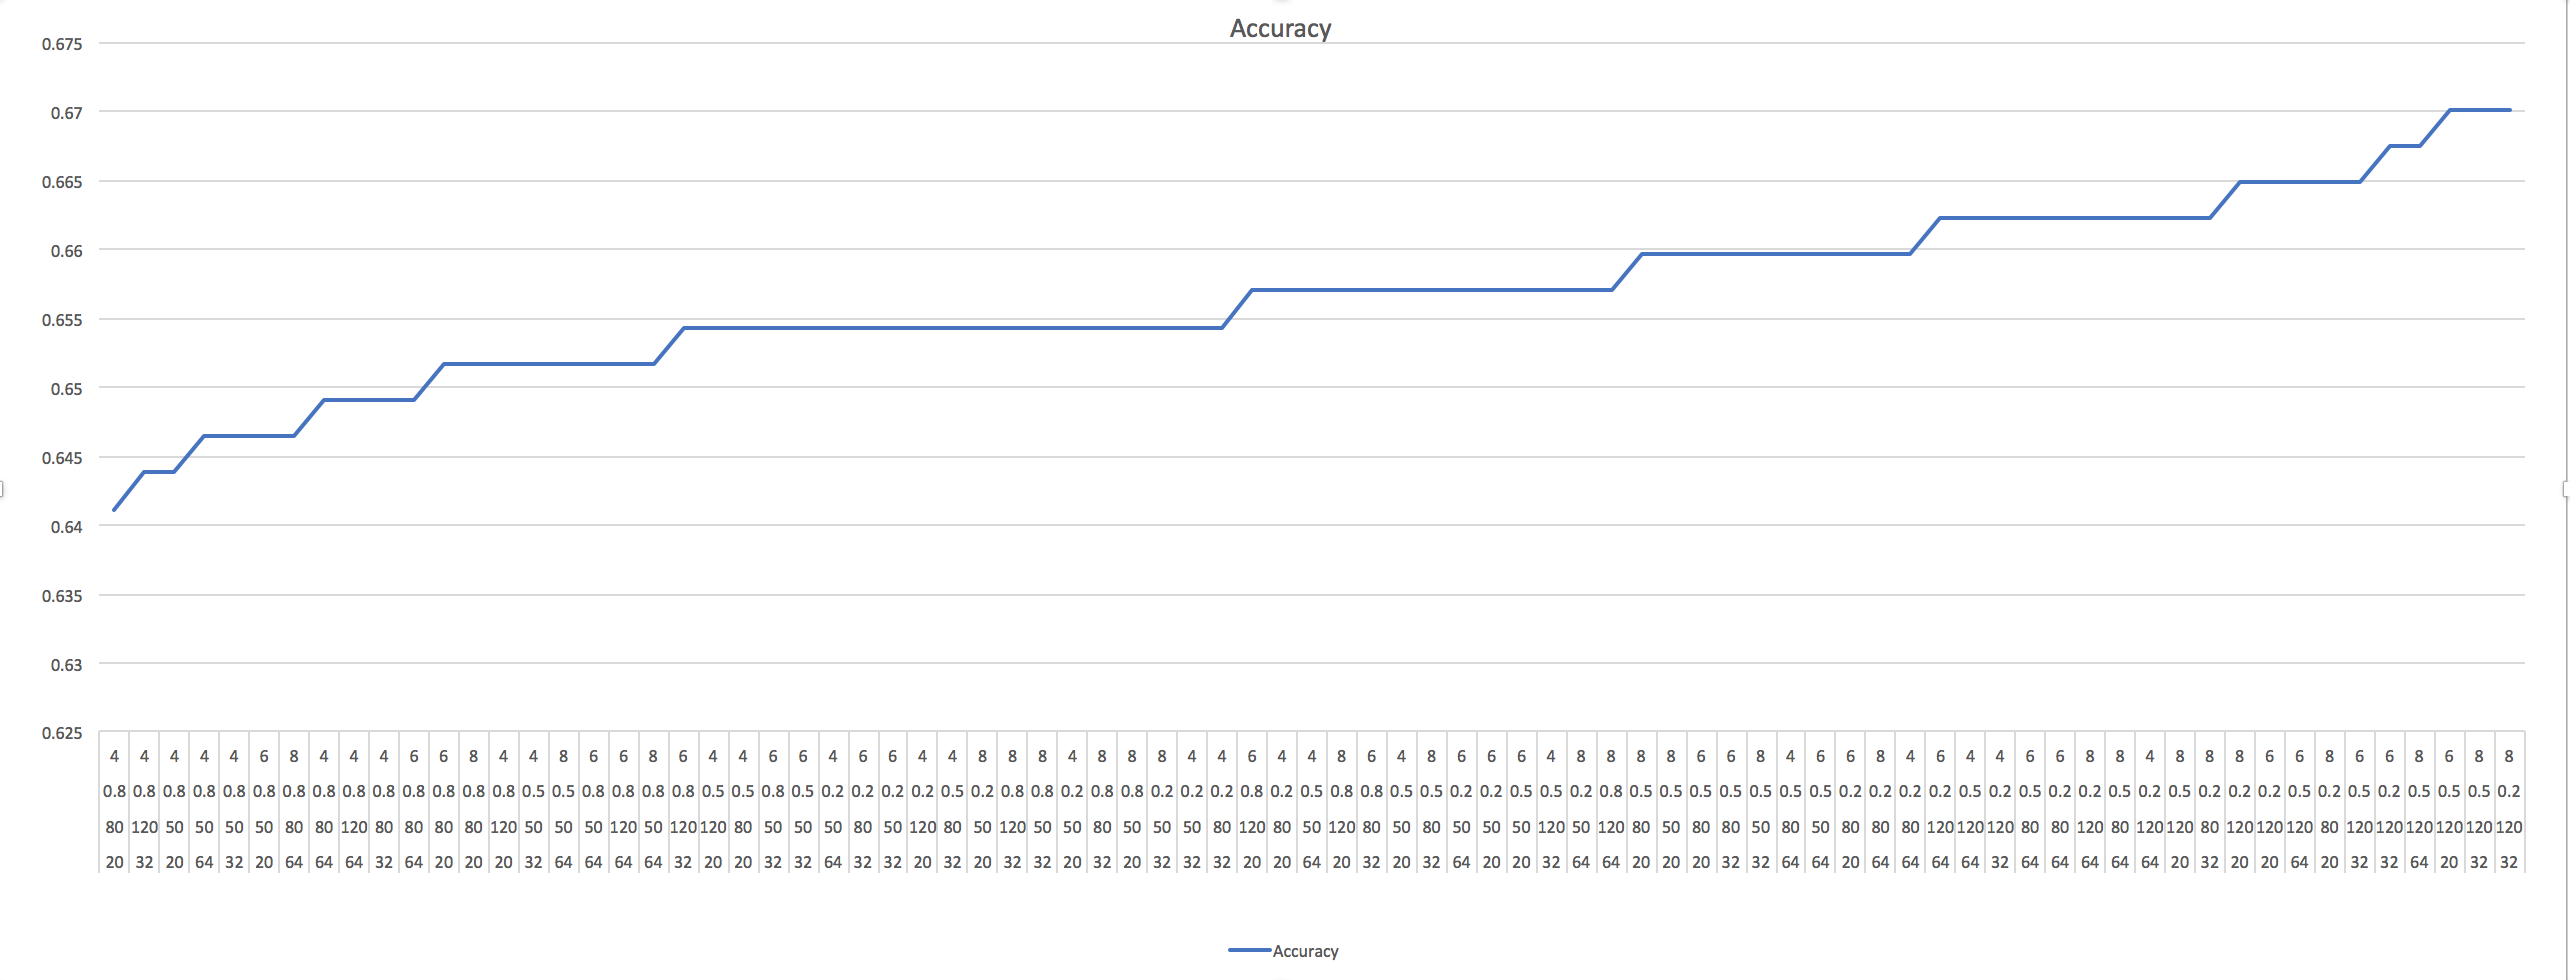
\includegraphics[width=14cm,height=8cm]{images/keras_grid_search_50.png}
\caption{Оптимизација на моделот преку пребарување за множество 50}
\label{fig:grid_search_50}
\centering
\end{figure}

\begin{table}[hbtp]
 \centering
 \scalebox{0.8}{%
 \begin{tabular}{| c | c |}
 \hline
 параметар & вредности \\ 
 \hline
 \hline
 batch\_size & 32\\ 
 \hline
 epochs & 50 \\ 
 \hline
 dropout & 0.2 \\ 
 \hline
 kernel\_constraint &  8 \\ 
 \hline
 hidden\_layers & 1 \\
  \hline
 neurons &  (влезна димезнија)*1 \\ 
 \hline
  activation & 'relu' за скриените слоеви, 'sigmoid' за излезниот слој \\ 
 \hline
 optimizer & 'adam' \\ 
 \hline
 loss & 'categorical\_crossentropy' \\ 
 \hline
\end{tabular}}
\caption{Оптимална конфигурација на моделот во Керас за податочно множество 49}
\label{table:params_conf_49}
\end{table}

\begin{table}[hbtp]
 \centering
 \scalebox{0.8}{%
 \begin{tabular}{| c | c |}
 \hline
 параметар & вредности \\ 
 \hline
 \hline
 batch\_size & 32\\ 
 \hline
 epochs & 120 \\ 
 \hline
 dropout & 0.5 \\ 
 \hline
 kernel\_constraint &  8 \\ 
 \hline
 hidden\_layers & 1 \\
  \hline
 neurons &  (влезна димезнија)*1 \\ 
 \hline
  activation & 'relu' за скриените слоеви, 'sigmoid' за излезниот слој \\ 
 \hline
 optimizer & 'adam' \\ 
 \hline
 loss & 'binary\_crossentropy'\\ 
 \hline
\end{tabular}}
\caption{Оптимална конфигурација на моделот во Керас за податочно множество 50}
\label{table:params_conf_50}
\end{table}

Во следниот чекор на тестирање ги користевме тренинг и валидациското множества како едно целосно тренинг множество и го евалуиравме моделот врз тест множеството. На сличен начин како и пребарувањето на вредностите на параметрите направивме пребарување со цел да најдеме најдобра архитектура на невронска мрежа за нашиот проблем. Пребарувавме низ бројот на неврони и вкупниот број на скриени слоеви. За двете податочни множества добивме најоптимална архитектура со еден скриен слој со ист број на неврони колку и влезниот слој. За множеството 49 добивме архитектура со 26 неврони во влезниот слој, 26 неврони во скриениот слој и 3 во излезниот прикажана на слика . За множеството 50 добивме архитектура со 18 неврони во влезниот слој, 18 неврони во скриениот слој и 1 во излезниот прикажана на слика . При нормализација на податоците најдобри резултати ни даде min-max во опсег од 0 до 1, додека пак при кодирањето ги пробавме бинарното и класното кодирање, каде класното кодирање постигна подобри резултати. 
За множеството 49 добивме точност од 55.91\% додека за множеството 50 добивме точност од 67.38\%.

\begin{figure}[H]
\centering
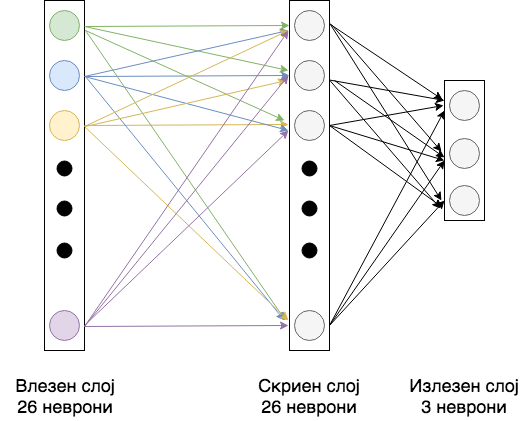
\includegraphics[scale=0.34]{images/Neural_net_49.png}
\caption{Архитектура на невронска мрежа за податочно множество 49}
\label{fig:architecture_49}
\centering
\end{figure}

\begin{figure}[H]
\centering
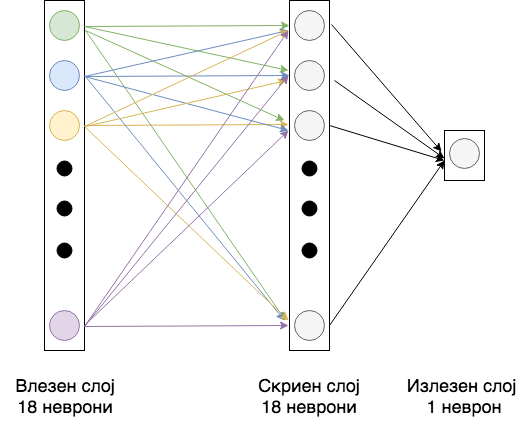
\includegraphics[scale=0.34]{images/Neural_net_50.png}
\caption{Архитектура на невронска мрежа за податочно множество 50}
\label{fig:architecture_50}
\centering
\end{figure}


\chapter{Евалуација на моделите}
\label{sec:evaluation}
Евалуација на моделите ни го одговара прашањето - Како да го одбереме најдобриот модел? Без разлика дали одбираме помеѓу различни алгоритми или ги одбираме оптималните параметри или одбираме помеѓу различни атрибути, нас ни треба процедура за евалуација на модели за да ни помогне да процениме колку добро еден модел ќе се генерализира на податоците што не бил трениран. Како и да е нам ни требаат и евалуациски метрики за да ги споредиме со нашите процедури за да можеме да ги квантифицираме перформансите на моделот.

Секогаш ни треба евалуациска метрика што ќе оди заедно со одбрана процедура и изборот на метрика зависи од типот на проблемот кој го решаваме. За регресивни проблеми користиме средна апсолутна грешка или средна квадратна грешка, додека за класификациски проблеми како нашиот досега користевме само класификациска точност. Постојат и други важни метрики кои ќе ги разгледаме во ова поглавје. 
\section{Класификациска точност}
Пред да ги проучиме другите евалуациски метрики, да ја разгледаме прво класификациската точност. За да ја добиеме класификациската точност ние во претходното поглавје го разделивме на тренинг, валидациско и тест множество. Со тренинг и валидациското множество ги наоѓавме најдобрите параметри за нашите модели каде како вредност што треба да ја максимизираме ја земавме точноста. Со тренинг и валидациското множество заедно го трениравме моделот и ги евалуиравме нашите резултати врз тест множеството исто така со точноста. Класификациската точност е всушност процентот на точните предвидувања. На слика \ref{fig:comparison_49} и слика \ref{fig:comparison_50} може да се видат точностите на сите алгоритми за соодветните податочни множества. Од резултатите можеме да забележиме дека за податочното множество 49 каде имаме 3 класи, моделите на екстремно случајни дрва и случајна шума ни даваат подобри резултати, веднаш по нив е моделот добиен со невронската мрежа. Кај множеството 50 каде имаме 2 класи, подобри резултати добиваме кај наивен баесов класификатор, логистичката регресија и машини со носечки вектори, но и моделот на невронските мрежи пак постигна добри резултати. Со ова можеме да заклучиме дека невронските мрежи и во двата случаи се добри предвидувачи.

\begin{figure}[H]
\centering
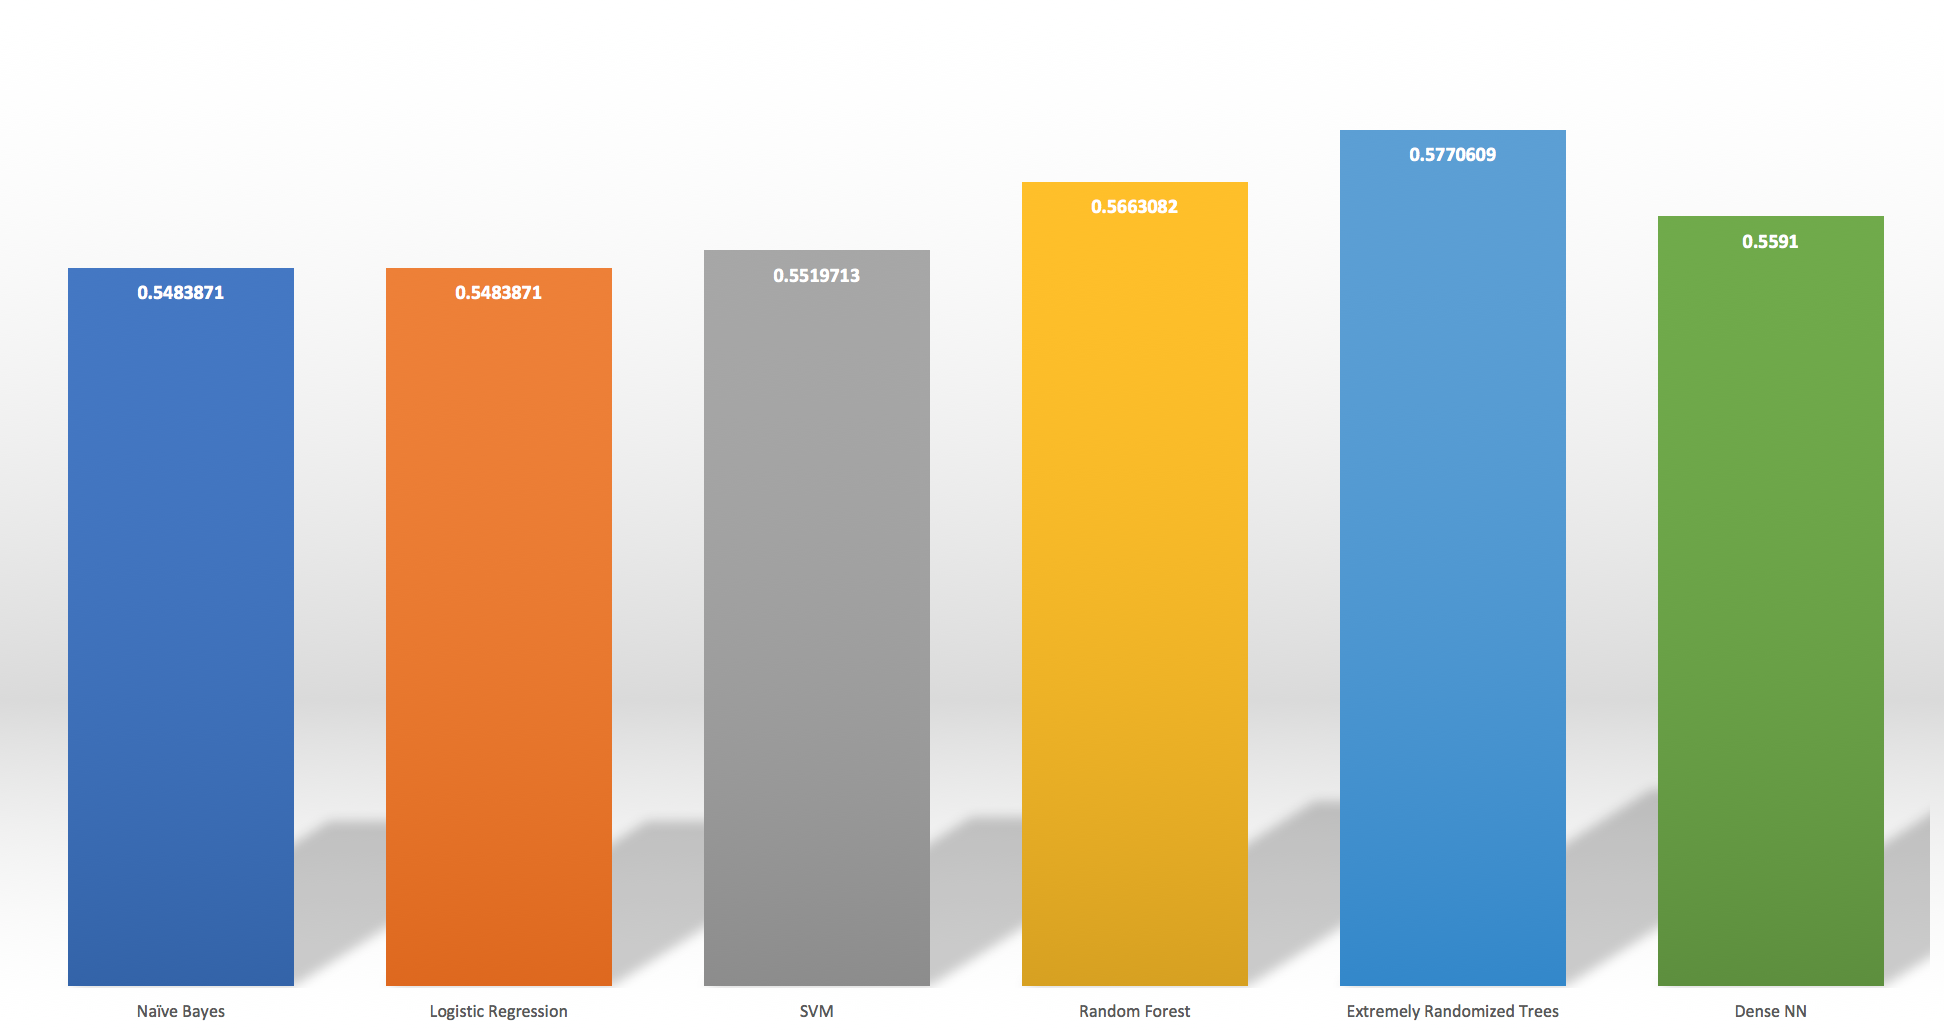
\includegraphics[scale=0.34]{images/comparison_algo_49.png}
\caption{Споредба на резултати од тестирање за податочно множество 49}
\label{fig:comparison_49}
\centering
\end{figure}

\begin{figure}[H]
\centering
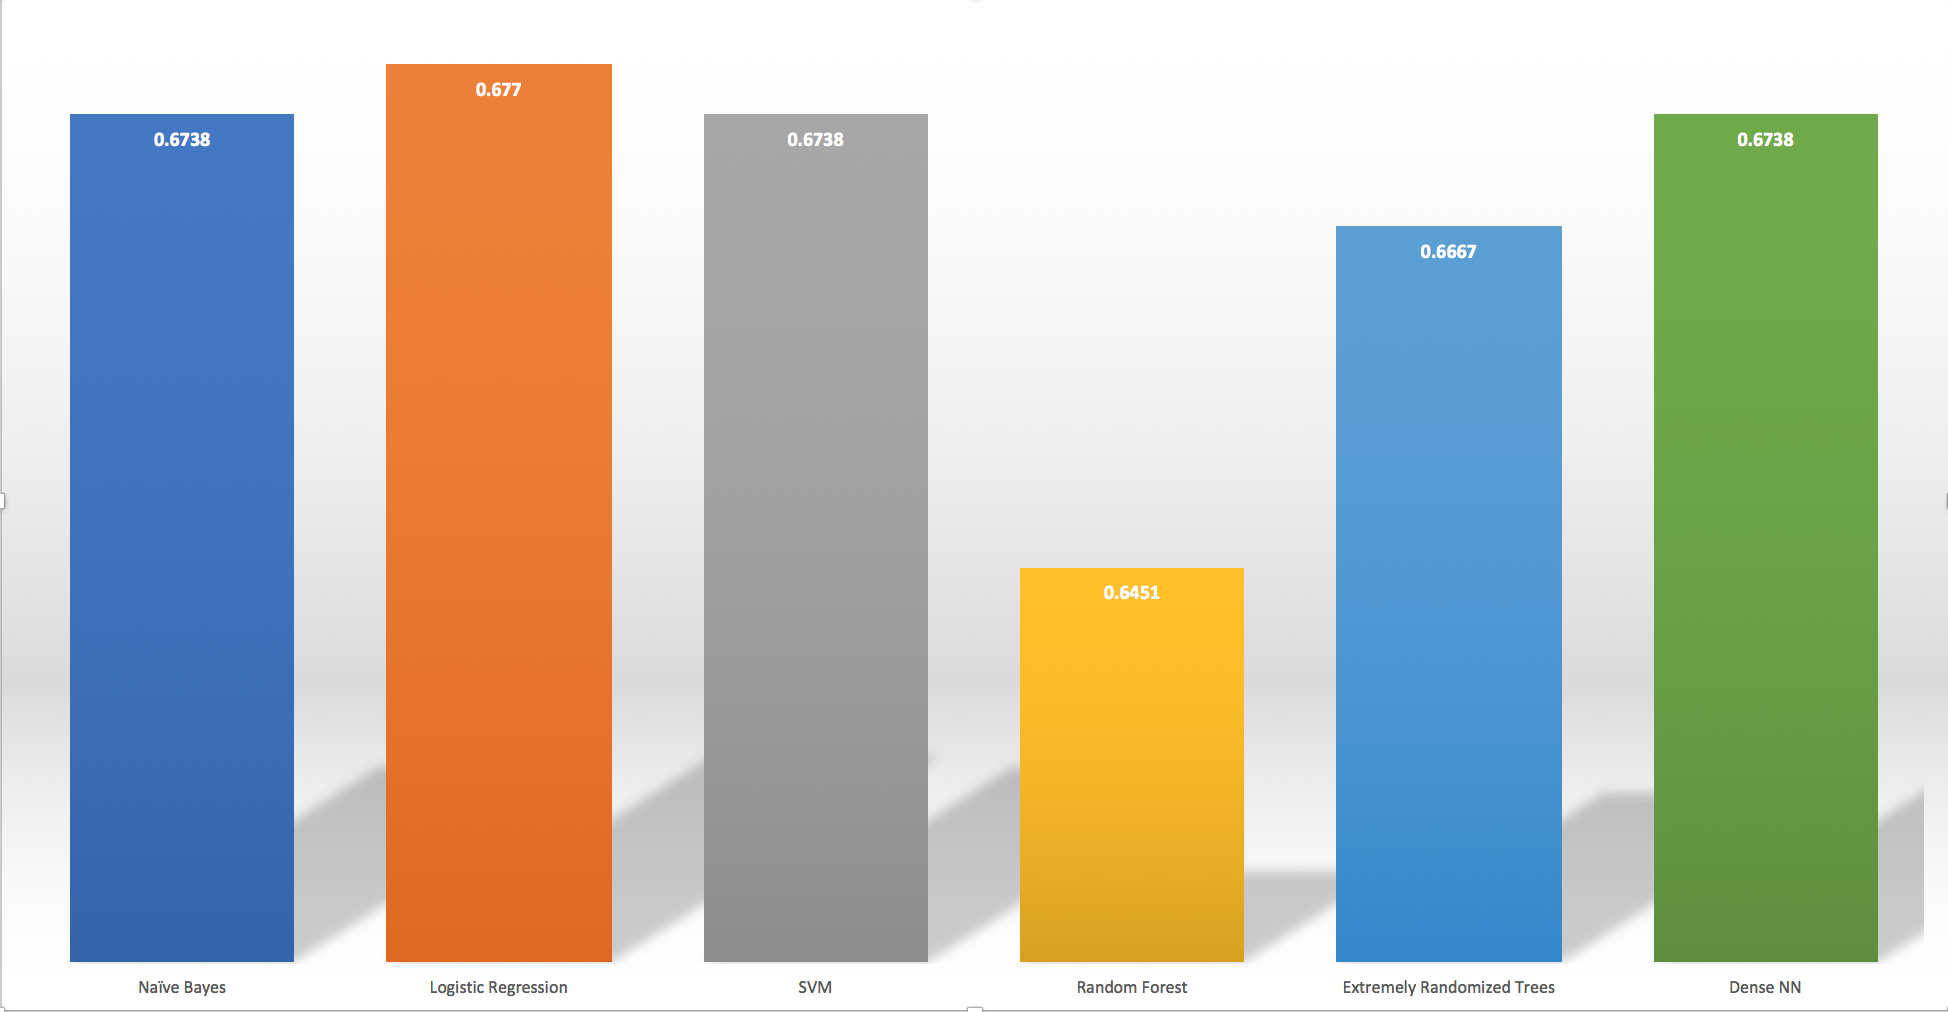
\includegraphics[scale=0.34]{images/comparison_algo_50.png}
\caption{Споредба на резултати од тестирање за податочно множество 50}
\label{fig:comparison_50}
\centering
\end{figure}


\section{Нулта точност}
Секогаш кога користиме класификациска точност, важно е да да ја споредиме со нулта точност. Нулта точност е точноста што може да ја постигниме со тоа што секогаш ќе ја предвидуваме најфреквентната класа во тест множеството. Ако ја пресметаме нултата точност за нашите податочни множества ќе видеме зошто ова е важна мeтрика. Кај множеството 49 имаме нулта точност од 45.52\% на класата 1, а кај можеството 50 имаме 54.48\% на класата Х2. На слика \ref{fig:null_acc_49} можеме да ја видеме споредбата на нултата точност во однос на другите алгоритми кај множеството 49, а на слика \ref{fig:null_acc_50} кај множеството 50. Од резултатите можеме да забележеме дека моделот на невронските мрежи и во двата случаи повторно ни дава добри резултати, за множеството 49 моделот е подобар за 10.4\%, а за множеството 50 за 12.9\%. Исто така овде многу добри резултати ни покажа и моделот на екстремно случајни дрва каде и во двата случаи резултатот од предвудувањата е подобар од нултата точност за 12.18\%.
\begin{figure}[H]
\centering
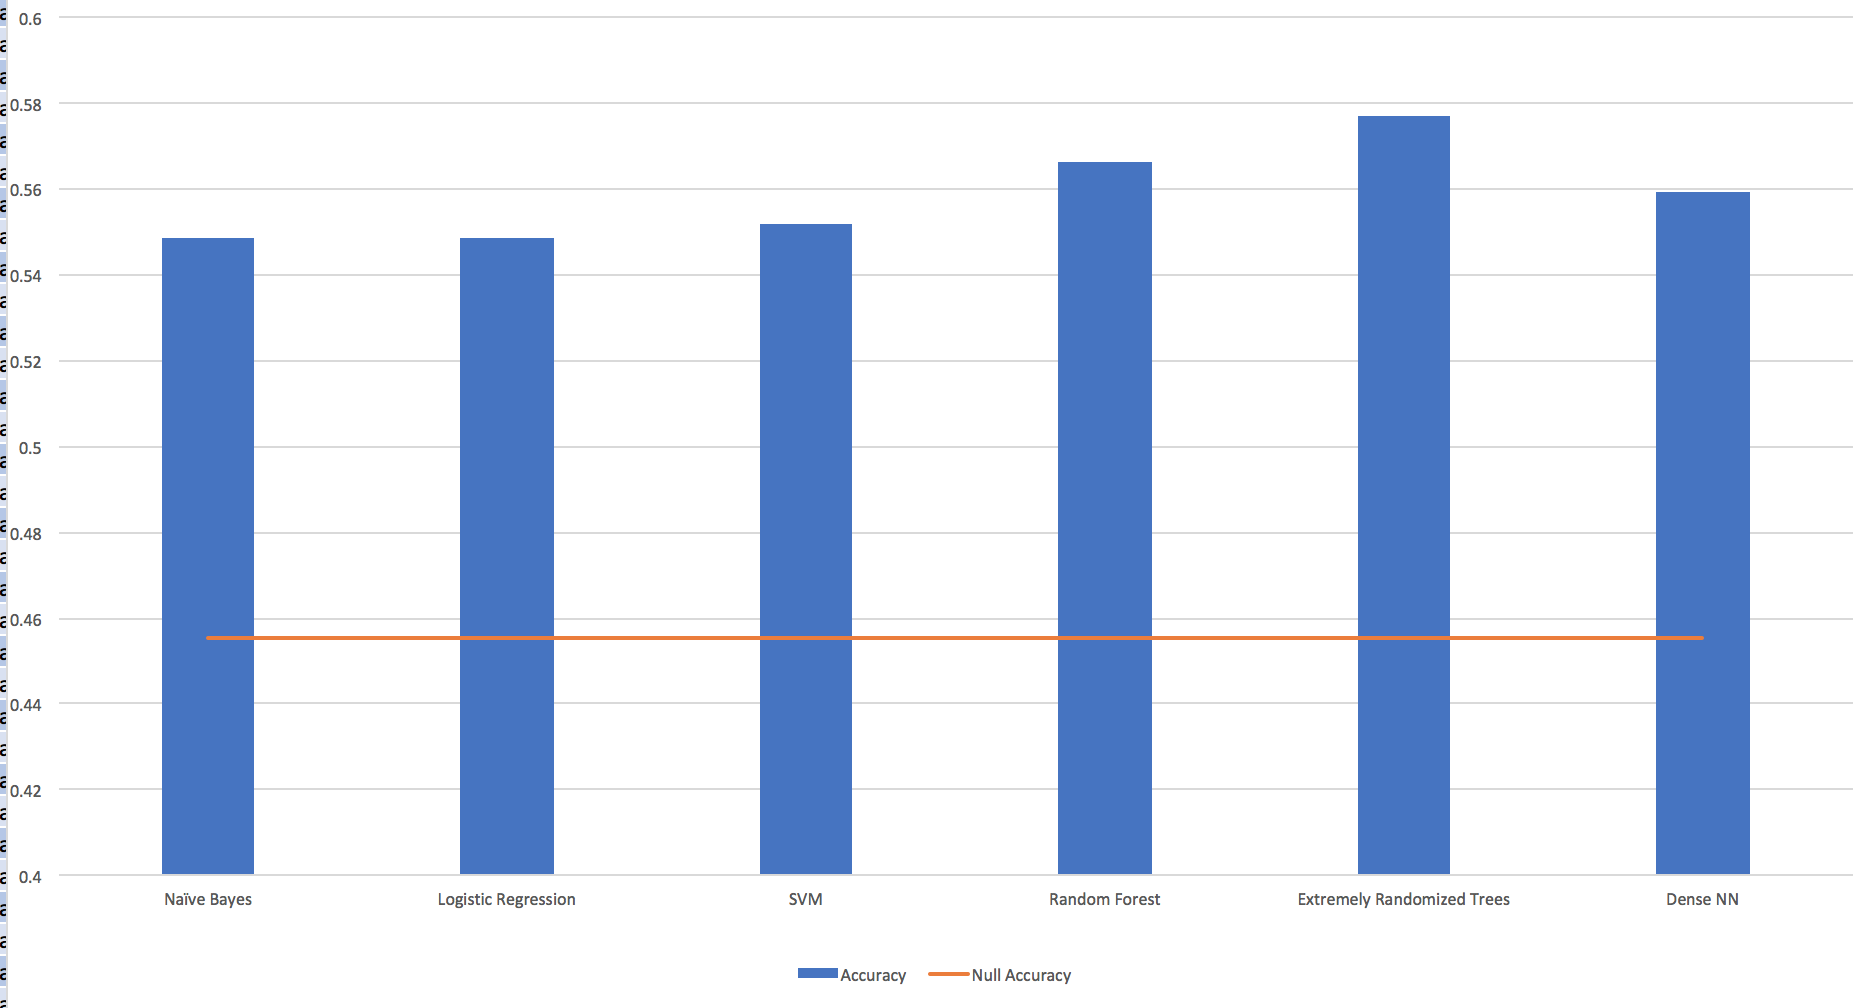
\includegraphics[scale=0.34]{images/null_accuracy_49.png}
\caption{Споредба на резултати од тестирање со нулта точност за податочно множество 49}
\label{fig:null_acc_49}
\centering
\end{figure}

\begin{figure}[H]
\centering
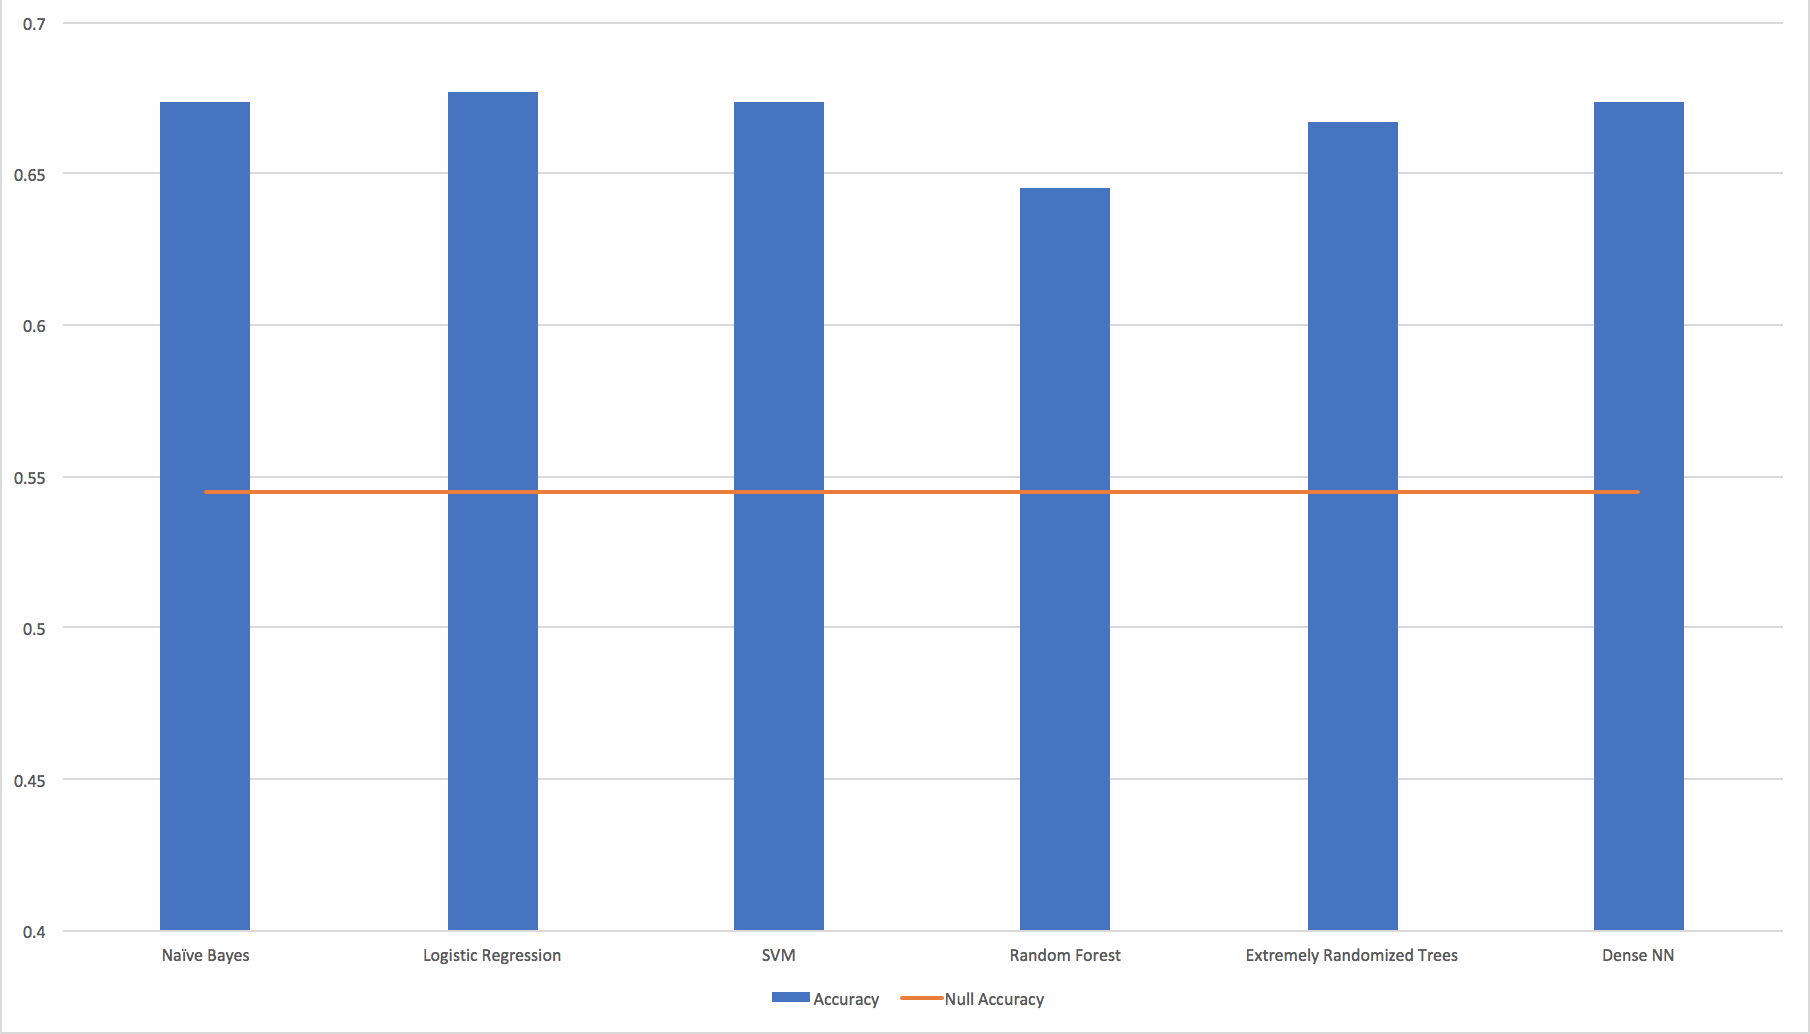
\includegraphics[scale=0.34]{images/null_accuracy_50.png}
\caption{Споредба на резултати од тестирање со нулта точност за податочно множество 50}
\label{fig:null_acc_50}
\centering
\end{figure}

\section{Матрица на забуни}
Матрицата на забуни е табела која ги опишува перформансите на еден класификацискиот модел. Матрицата е со големина k*k каде k е бројот на класи. 
\begin{table}[H]
 \centering
 \scalebox{0.8}{%
 \begin{tabular}{| c | c | c |}
 \hline
 & Предвидено = 0 & Предвидено = 1 \\
  \hline
 Реално = 0 & TN & FP \\
 Реално = 1 & FN & TP \\
 \hline
\end{tabular}}
\caption{Пример на матрица на забуни}
\label{table:confusion_mat_example}
\end{table}

На табела \ref{table:confusion_mat_example} е прикажана матрица на забуни за бинарен проблем, и кога се користи за ваков тип на класификација секој елемент од матрицата има специфично име:
\begin{itemize}
  \item Точно позитивно (True Positive, TP анг,): Броjот на точни придвидувања дека инстанцата е позитивна.
  \item Точно негативно (True Negative,TN анг.): Броjот на точни предвидувања дека инстанцата е негативна.
 \item Неточно позитивно (False Positive, FP анг.): Броjот на неточни предвидувања дека инстанцата е позитивна.
 \item Неточно негативно (False Negative, FN анг.): Броjот на неточни предвидувања дека инстанцата е негативна.
\end{itemize}
Матрицата на забуни се користи за да ни помогне подобро да ја разбереме работата на нашиот модел, но од неа директно не можеме да одбериме кој модел е подобар, бидејќи не е метрика за евалуација на модел. Како и да е, постојат метрики кои можат да бидат пресметани од матрица на забуни, и тие може директно да се искористат да се одбере најдобар модел. Ќе разгледаме неколку од популарните метрики и на крај ќе одбереме која метрика да ја оптимизираме.

Една од наједноставните и најочигледните метрики што можеме да ги пресметаме со матрица на забуни е точноста претставена како:
\begin{equation}
\frac{TP + TN}{TP + FP + FN + TN}
\end{equation}
Следната метрика е рата на грешка односно колку често класификаторот направил погрешно предвидување:
\begin{equation}
\frac{FP + FN}{TP + FP + FN + TN}
\end{equation}

Рата на точно позитивно предвидување или уште познато како осетливост (sensitivity, recall, hit rate, or true positive rate, анг.):

\begin{equation}
TPR = \frac{TP}{TP + FN}
\end{equation}

Рата на неточно позитивно предвидување (false positive rate оr fall-out, анг.):

\begin{equation}
FPR = \frac{FP}{TN + FP}
\end{equation}

Рата на точно негативно предвидување (specificity or true negative rate, анг.):

\begin{equation}
TNR = \frac{TN}{FP +TN}
\end{equation}

Рата на неточно негативно предвидување или промашување (miss rate or false
negative rate анг.):

\begin{equation}
FNR = \frac{FN}{FN + TP}
\end{equation}


Прецизност (precision or positive predictive value, анг.), односно колку често предвидениот излез е точен:
\begin{equation}
\frac{TP}{TP + FP}
\end{equation}

Доколку броjот негативни случаи е значително поголем од броjот на позитивни случаи, тогаш овие пресметки ќе посочат каде настанува грешка.
Во нашите случаи исто така ги применивме горните равенки за да ги најдеме дополнителните метрики кои ќе ни требаат за следниот чекор а тоа е градење на стратегија на обложување. Метриките за множество 49 и множество 50 се прикажани на табела \ref{table:metrics_49} и табела \ref{table:metrics_50} соодветно.

\begin{table}[H]
 \centering
 \scalebox{0.5}{%
 \begin{tabular}{| c | c | c | c | c | c | c | c | c |}
 \hline
 класификатор & точност & рата на грешка & осетливост 1 & осетливост X & осетливост 2 & прецизност 1 & прецизност X & прецизност 2 \\
  \hline
 NaiveBayes & 0.5483 & 0.4516 & 0.5467	& 0 & 	0.8819 & 0.4940 &	0 &	0.5714\\
 LogisticRegression & 0.54838 & 0.4516 & 0.8740 & 0.56 & 0.0 & 0.5663 & 0.5060 & 0.0\\
 SVM & 0.5519& 0.4480 & 0.8740 & 0.5733 & 0.0 & 0.5692 & 0.5119 & 0.0 \\
 RandomForest & 0.5663 & 0.4336 & 0.7637 & 0.5733 & 0.2337 & 0.6024 & 0.5243 & 0.5 \\
 ExtremelyRandomizedTrees & 0.5770 & 0.4229 & 0.8031 & 0.56 & 0.2207 & 0.5964 & 0.5675 & 0.5\\
 NeuralNet & 0.5591 & 0.4408 & 0.8661 & 0.0649 & 0.5466 & 0.5555 & 0.7142 & 0.5540 \\
 \hline
\end{tabular}}
\caption{Изведени метрики од матрица на забуни за множество 49}
\label{table:metrics_49}
\end{table}

\begin{table}[H]
 \centering
 \scalebox{0.8}{%
 \begin{tabular}{| c | c | c | c | c |}
 \hline
 класификатор & точност & рата на грешка & осетливост & прецизност \\
  \hline
 NaiveBayes & 0.6451 & 0.3548 & 0.6535 & 0.6014 \\
 LogisticRegression & 0.6774 & 0.3225 & 0.5511 & 0.6796 \\
 SVM & 0.6738 & 0.3261 & 0.5039 & 0.6956 \\
 RandomForest & 0.6738 & 0.3261 & 0.5196 & 0.6875 \\
 ExtremelyRandomizedTrees & 0.6666 & 0.3333 & 0.5354 & 0.6666 \\
 NeuralNet & 0.6738 & 0.3261 & 0.5039 &  0.6956 \\
 \hline
\end{tabular}}
\caption{Изведени метрики од матрица на забуни за множество 50}
\label{table:metrics_50}
\end{table}

Добра практика е секогаш да ја испитуваме матрицата на забуни бидејќи ни дава целосна слика колку е ефикасен нашиот класификатор. Исто така ни дозволува да пресметаме различни класификациски метрики кои може да не насочат кон одбирање на подобар класификациски модел. 

\section{Стратегија}

Откако ја анализиравме точноста на моделите и метриките што се изведуваат од матрицата на забуни, можеме да предложиме стратегија за максимизирање на добивката на корисниците на нашиот систем. Просечниот обложувач претежно се обложува на повеќе натпревари на еден влог со надеж дека тоа ќе ја зголеми неговата добивка. Обложувалниците со тоа нудат зголемување на квотата на уплатата со тоа што вкупната квота што ја добива обложувачот е производ од сите квоти за кои тој типува и добивката изгледа примамлива. Со ваквиот начин на уплата од друга страна се намалува веројатноста на добивка. Од надежност на системи \cite{fussell1975hand} познато е дека доколку имаме повеќе компоненти во системот, во нашиот случај типувања на натпревари, надежноста на системот се намалува, пресметана со,

\begin{equation}
P= P_1\\P_2\\...P_n
\end{equation}

 каде n е бројот на компоненти на системот, а P\textsubscript{x} е надежноста на компонентата. Поради ваквата поставеност, нашата стратегија се базира на посебен влог на секое типување и со тоа шансата на загуба зависи само од една компонента. Резултатите од симулациите што ги направивме се прикажани на табела \ref{table:win_sim_49} и табела \ref{table:win_sim_50}. Од резултатите можеме да забележиме дека кај множесвото 50 за сите модели добиваме позитивни резултати.
 
  \begin{table}[H]
 \centering
 \scalebox{0.8}{%
 \begin{tabular}{| c | c |}
 \hline
 класификатор & добивка \\
  \hline
 NaiveBayes & -3.15\%  \\
 LogisticRegression & -5.19\%  \\
 SVM & -11.68\%  \\
 RandomForest & +4.67\% \\
 ExtremelyRandomizedTrees & -3.04\% \\
 NeuralNet & -3.04\%  \\
 \hline
\end{tabular}}
\caption{Симулација на добивка за множеството 49}
\label{table:win_sim_49}
\end{table}
 
 \begin{table}[H]
 \centering
 \scalebox{0.8}{%
 \begin{tabular}{| c | c |}
 \hline
 класификатор & добивка \\
  \hline
 NaiveBayes & +1.6\%  \\
 LogisticRegression & +2.83\%  \\
 SVM & +1.8\%  \\
 RandomForest & +2.23\% \\
 ExtremelyRandomizedTrees & +2.2\% \\
 NeuralNet & +1.6\%  \\
 \hline
\end{tabular}}
\caption{Симулација на добивка за множеството 50}
\label{table:win_sim_50}
\end{table}

\section{Прилагодување на прагот на класификација}

За да ја подобриме добивката на системот треба да ги погледнеме метриките изведени од матрицата на забуни и како би ни користеле во нашиот случај. Изборот на метриката на која сакаме да оптимизираме зависи од нашата бизнис цел, дали сакаме да ја оптимизираме презицноста на нашиот модел или осетливоста. Кај еден ваков систем на препораки целта е да се намалат неточните позитиви (false positive анг.), затоа ќе се фокусираме кон зголемувањето на прецизноста на нашиот модел. За да ја зголемиме прецизноста на моделите го зголемуваме прагот на класификација, со тоа класата ќе биде препознаена доколку го надмине прагот кој ќе го поставиме. Доколку ниедна класа не го надминува поставениот праг, тој натпревар нема да го земеме во предвид. На слика \ref{fig:thresh_simulation_50} е прикажан графикот од симулацијата на множеството 50, за различни прагови и вкупната добивка изразена во проценти. На табела  \ref{table:win_sim_50_0_8} е претставена финалната симулација и потенцијалните добивки од ваквиот систем. Од резултатите можеме да заклучиме дека со зголемувањето на прагот на класификација забележуваме раст на добивката. 

\begin{figure}[H]
\centering
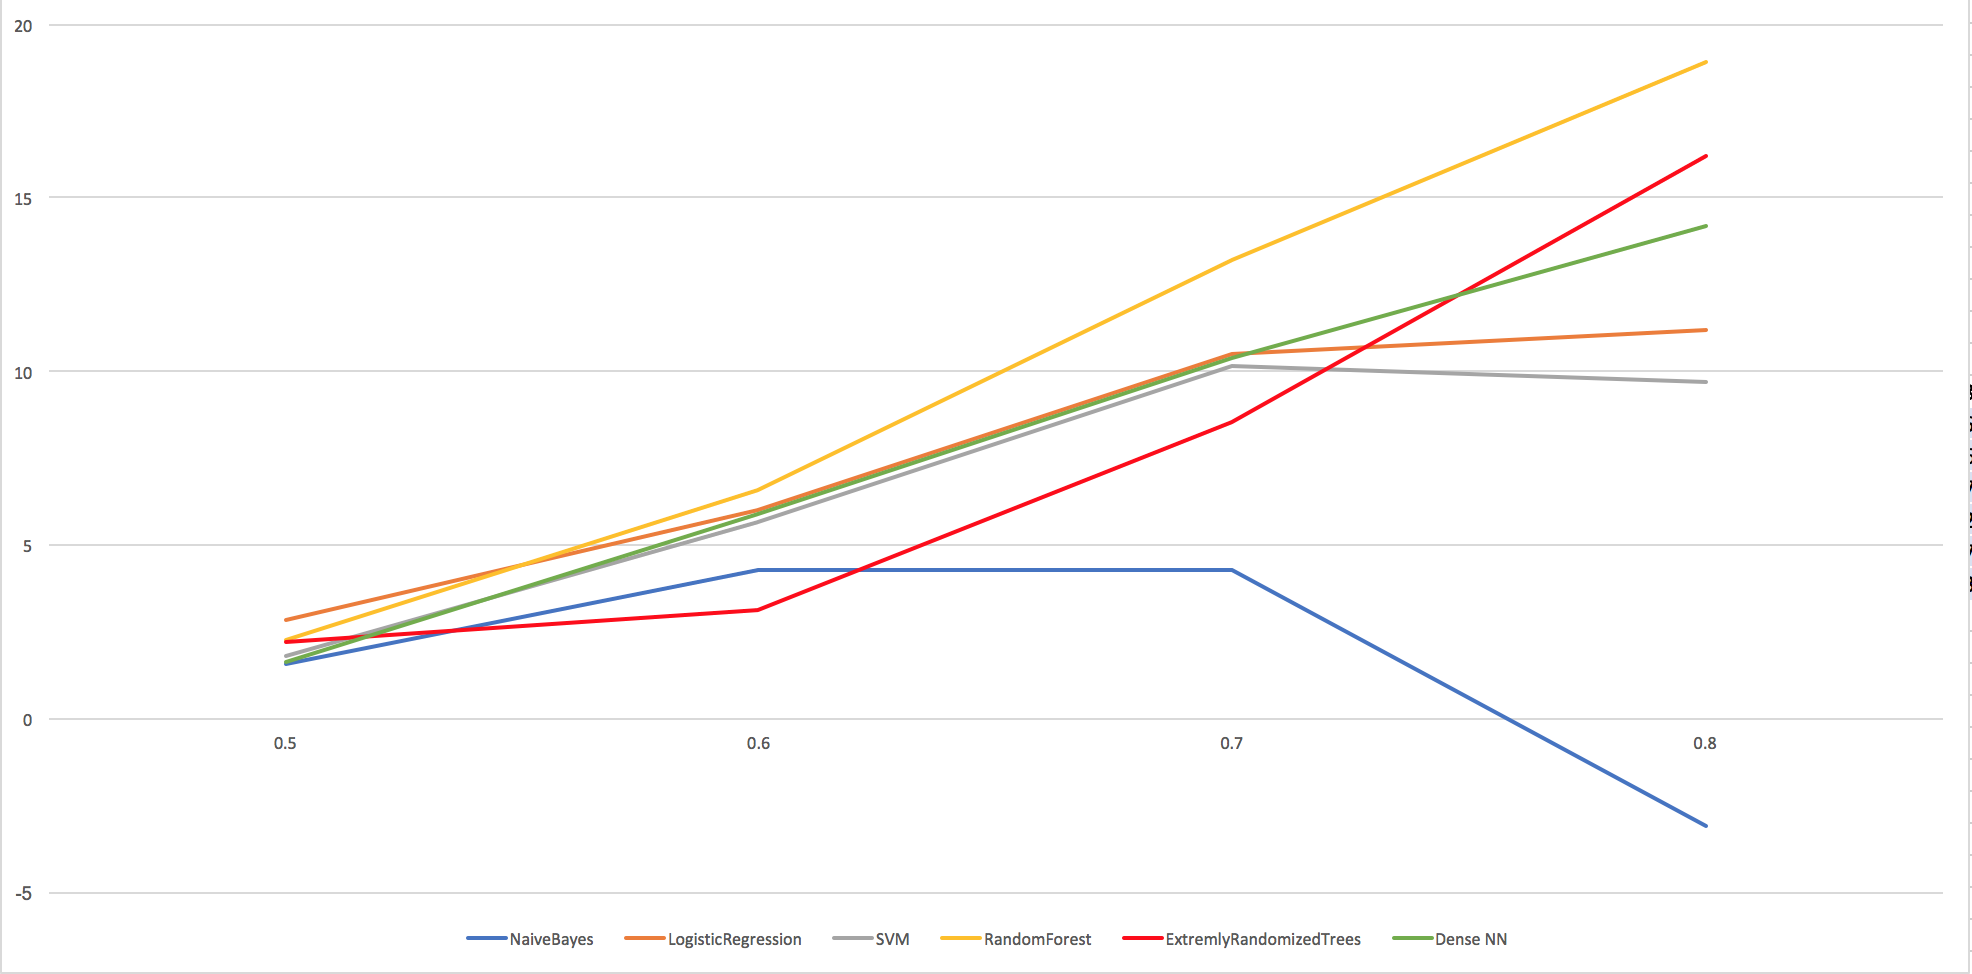
\includegraphics[scale=0.34]{images/thresh_simulation_50.png}
\caption{Симулација на добивка по различни прагови за множество 50}
\label{fig:thresh_simulation_50}
\centering
\end{figure}

 \begin{table}[H]
 \centering
 \scalebox{0.8}{%
 \begin{tabular}{| c | c |}
 \hline
 класификатор & добивка \\
  \hline
 NaiveBayes & -3.08\%  \\
 LogisticRegression & +11.21\%  \\
 SVM & +9.67\%  \\
 RandomForest & +18.89\% \\
 ExtremelyRandomizedTrees & +16.21\% \\
 NeuralNet & +14.20\%  \\
 \hline
\end{tabular}}
\caption{Симулација на добивка за множеството 50 со праг на класификација од 0.8}
\centering
\label{table:win_sim_50_0_8}
\end{table}

\section{Исплатливост}

Со моделите на случајни шуми, екстремно случајни дрва и невронските мрежи забележувме значителна добивка. За споредба банкарските камати на орочување од 1 до 5 години се движат од 1.2\% до 3.6\%, додека нашиот систем произведува заработка од 14\% до 18\% од целосниот влог. Сепак овој начин на заработка е доста ризичен и не можеме да го одобриме и покрај добрите резултати.

\chapter{Заклучок и идна работа}
\label{sec:conclusion}

Во овој магистерски труд главна тема беше предвидувањето на резултати од спортски натпревари со помош на алгоритми за машинско учење, каде главниот фокус беа на невронските мрежи. Дознавме дека за да се направи успешен систем за препораки се потребни повеќе процеси кои беа разгледани во текот на ова истражување.

Во глава \ref{sec:architecture} беше разгледана архитектурата на системот за препораки, каде поминавме низ процесот на дизајнирање на системи. Ги разгледавме кои се корисничките сценарија и огранучувањата на еден ваков систем. Беше понуден апстрактен дизајн на системот и подобрувања за справувања со тесни грла. Со ова се доби јасна претстава кои се најпотребните компоненти за еден ваков систем да работи.

Во глава \ref{sec:data} беа обработени две кориснички сценарија превземање и обработка на податоците. Покажано беше дека за еден ваков систем да работи пред сè се потребни податоци, но потребни се добри податоци. При обработката на податоци беа применети неколку техники за промена на податоците и податочното множество со цел да добиеме подобри резултати во следните чекори.

Во глава \ref{sec:machine_learning} беа разгледани повеќе алгоритми за машинско учење кои служеа како репер за вештачките невронски мрежи. Разгледани беа алатките потребни за креирање на модел за вештачки невронски мрежи и техники за добивање на најдобрите параметри и најдобрата архитектура. Беше претставена густо поврзаната невронска мрежа како архитектура која најдобро го решава проблемот на функциско мапирање и како овој алгоритам се справува со проблемот во однос на другите алгоритми.

Во глава \ref{sec:evaluation} се направи евалуација на разултатите од моделите на класификација. Овде беше покажано дека кај еден класификациски модел не е доволно само тренирање и тестирање на податоците и со тоа добивање на точност. Прво, беа споредени резутатите со нултата точност да се види дали моделите добро го решаваат проблемот. Беше разгледана матрицата на забуни како алатка која дава целосна слика на еден класификациски модел и од која може да се изведат дополнителни метрики кои може да се оптимизираат со цел да се постигне одредена бизнис цел. На крај беше изградена стратегија на системот и беше оптимизирана со помош на метриките од матрицата на забуни. Со тоа беше максимизиран профитот на потенцијалните корисници на системот.

Во денешно време освен обложувањето на спортски натпревари, постојат постојат повеќе места на кои луѓето гледаат како начин на брза заработка на пари. Таков пример се берзите за криптовалути.

